%%%%%%%%%%%%%%%%%%%%%%%%%%%%%%%%%%%%%%%%%
% Masters/Doctoral Thesis LaTeX Template
% Original authors: Steven Gunn and Sunil Patel
% Note: Make sure to edit document variables in the Thesis.cls file
%%%%%%%%%%%%%%%%%%%%%%%%%%%%%%%%%%%%%%%%%

%----------------------------------------------------------------------------------------
%	PACKAGES AND OTHER DOCUMENT CONFIGURATIONS
%----------------------------------------------------------------------------------------

\documentclass[11pt,twoside,a4paper]{Thesis} % The default font size and one-sided printing (no margin offsets)

\graphicspath{{figs/}} % Specifies the directory where pictures are stored

%\DeclareCiteCommand{\myparencite}[\mkbibparens]
%  {\usebibmacro{prenote}}
%  {\def\nameyeardelim{\addcomma\addspace}%
%   \usebibmacro{citeindex}%
%   \usebibmacro{cite}%
%   \def\nameyeardelim{\addspace}}
%  {\multicitedelim}
%  {\usebibmacro{postnote}}
%  
%\newcommand{\citeay}[1]{\citeauthor{#1} ({\citeyear{#1}})}

% some math symbols
\newcommand{\hzerooneOm}{{H_0^1(\Omega)}}
\newcommand{\hzerooneom}{{H_0^1(\omega)}}
\newcommand{\honeOm}{{H^1(\Omega)}}
\newcommand{\honeom}{{H^1(\omega)}}
\newcommand{\lpOm}[1]{{L^{#1}(\Omega)}}
\newcommand{\lpom}[1]{{L^{#1}(\omega)}}
\newcommand{\parder}[2]{\frac{\partial #1}{\partial #2}}

\newcommand{\wmp}[2]{{W^{#1,\,#2}(\Omega)}}
\newcommand{\veca}[1]{\vec{\mathbf{#1}}}
\newcommand{\vecb}[1]{\vec{\boldsymbol{#1}}}
\newcommand{\bds}[1]{\boldsymbol{#1}}
\usepackage{textcomp}
\addbibresource{lubric2013.bib}
\addbibresource{extras.bib}

%\usepackage[square, numbers, comma, sort&compress]{natbib} % Use the natbib reference package - read up on this to edit the reference style; if you want text (e.g. Smith et al., 2012) for the in-text references (instead of numbers), remove 'numbers' 
\hypersetup{urlcolor=blue, colorlinks=true} % Colors hyperlinks in blue - change to black if annoying

\title{\ttitle} % Defines the thesis title - don't touch this

\begin{document}

\frontmatter % Use roman page numbering style (i, ii, iii, iv...) for the pre-content pages

\setstretch{1.3} % Line spacing of 1.3

% Define the page headers using the FancyHdr package and set up for one-sided printing
\fancyhead{} % Clears all page headers and footers
\rhead{\thepage} % Sets the right side header to show the page number
\lhead{} % Clears the left side page header

\pagestyle{fancy} % Finally, use the "fancy" page style to implement the FancyHdr headers

\newcommand{\HRule}{\rule{\linewidth}{0.5mm}} % New command to make the lines in the title page

% PDF meta-data
\hypersetup{pdftitle={\ttitle}}
\hypersetup{pdfsubject=\subjectname}
\hypersetup{pdfauthor=\authornames}
\hypersetup{pdfkeywords=\keywordnames}

%----------------------------------------------------------------------------------------
%	TITLE PAGE
%----------------------------------------------------------------------------------------
% include the ICMC cover template
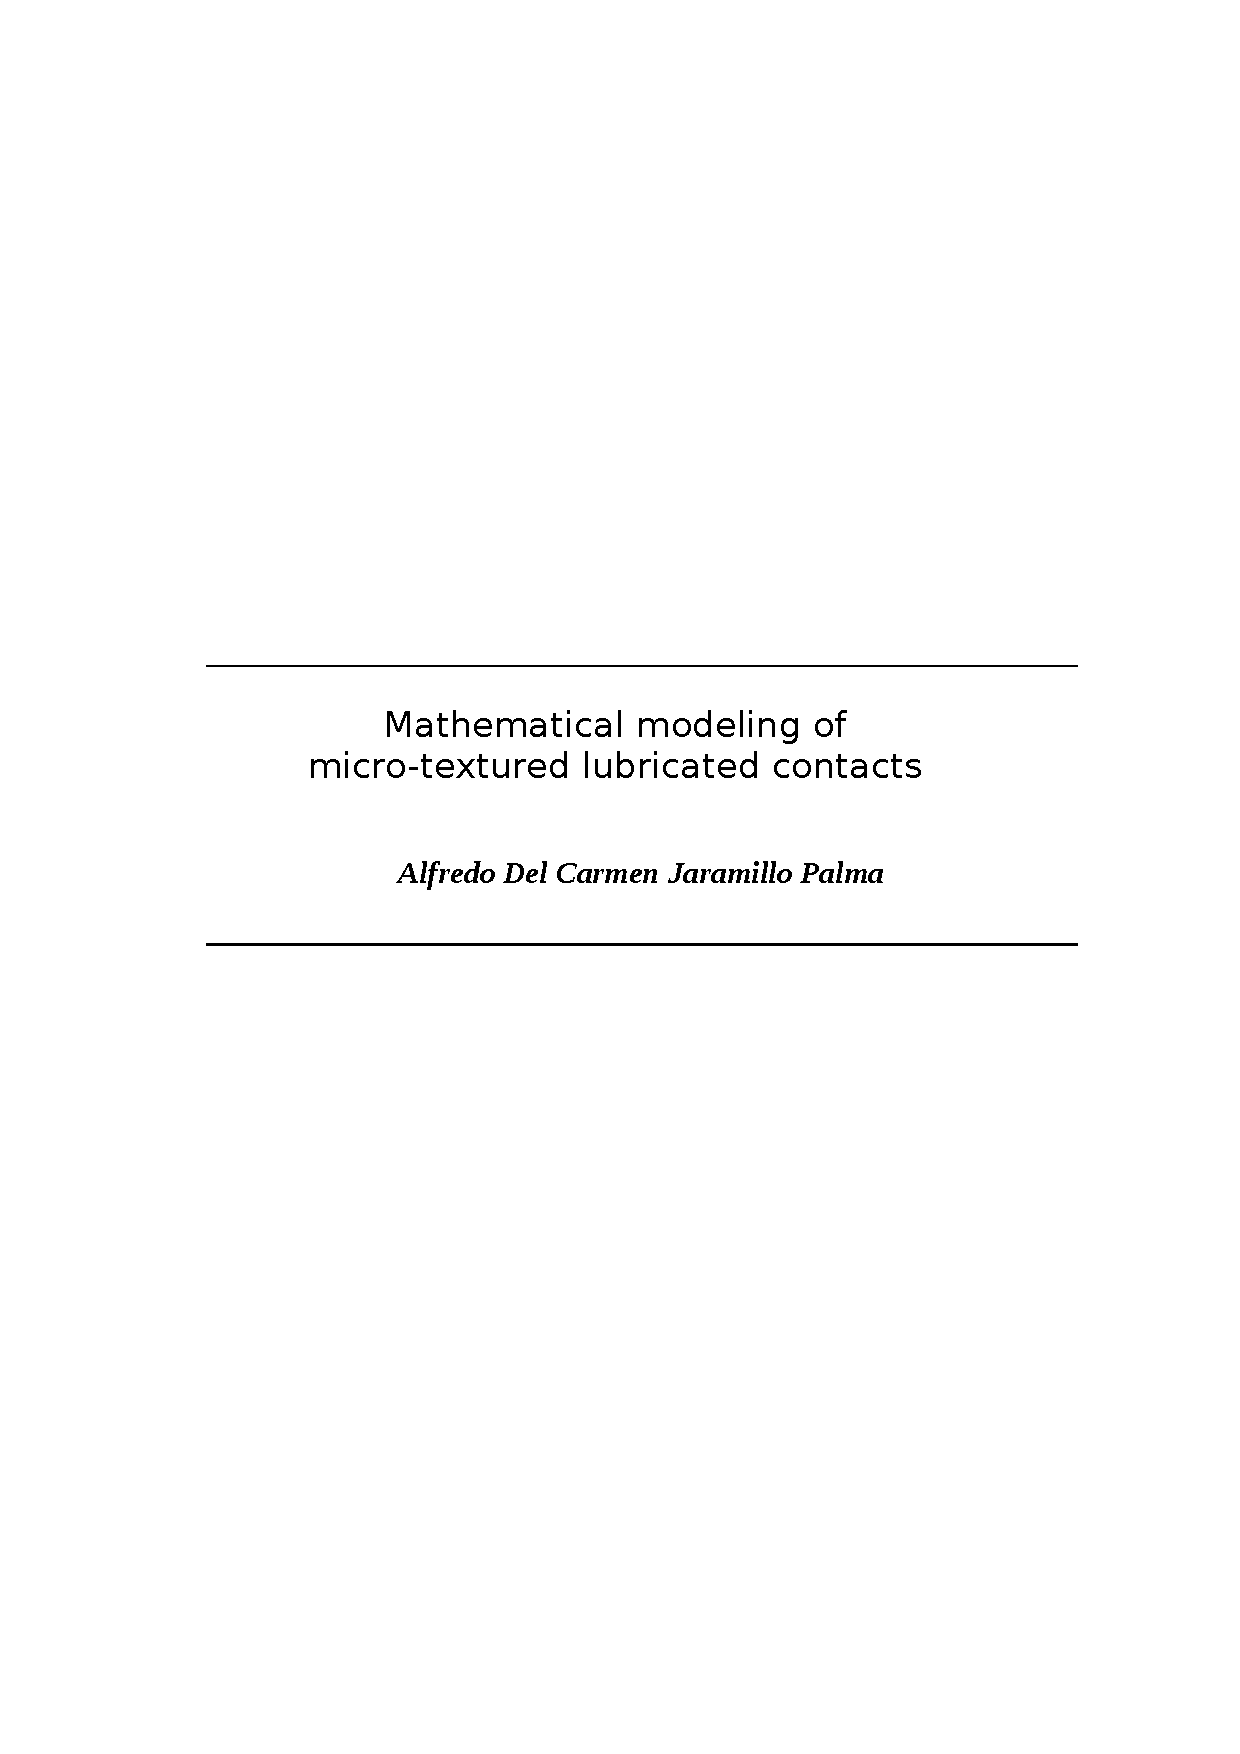
\includepdf[pages={1,2,3}]{portada}

\thispagestyle{empty}
\mbox{}
\pagestyle{empty}
\newpage

%----------------------------------------------------------------------------------------
%	QUOTATION PAGE
%----------------------------------------------------------------------------------------

\null\vfill % Add some space to move the quote down the page a bit

\textit{``\ldots La copa se hundió en el sol. Recogió un poco de la carne de Dios, la sangre del universo, el pensamiento deslumbrante, la enceguecedora filosofía que había amamantado a una galaxia, que guiaba y llevaba a los planetas por sus campos y emplazaba o acallaba vidas y subsistencias \ldots"}
\begin{flushright}
\textit{{\bf Las doradas manzanas del sol}, Ray Bradbury.}
\end{flushright}

\vfill\vfill\vfill\vfill\vfill\vfill\null % Add some space at the bottom to position the quote just right

\clearpage % Start a new page

%----------------------------------------------------------------------------------------
%	ABSTRACT PAGE
%----------------------------------------------------------------------------------------

\addtotoc{Abstract} % Add the "Abstract" page entry to the Contents

\abstract{\addtocontents{toc}{} % Add a gap in the Contents, for aesthetics

The Thesis Abstract is written here (and usually kept to just this page). The page is kept centered vertically so can expand into the blank space above the title too\ldots
}

\clearpage
\thispagestyle{empty}\null\vfil
\begin{center}
\setlength{\parskip}{0pt}
{\huge{\textit{Resumo}} \par}
\end{center}
Resumo\ldots
\clearpage % Start a new page

%----------------------------------------------------------------------------------------
%	ACKNOWLEDGEMENTS
%----------------------------------------------------------------------------------------

\setstretch{1.3} % Reset the line-spacing to 1.3 for body text (if it has changed)

\acknowledgements{\addtocontents{toc}{} % Add a gap in the Contents, for aesthetics
Agradezco a mis padres, quienes a la distancia me han apoyado durante este proceso, como durante toda mi vida; a Paola, por su cariño, paciencia y apoyo;\break a Hugo Checo, colega de pesquisa, y al profesor Mohammed Jai, por su ayuda y disposición; a Gustavo Buscaglia, mi orientador, por compartir su visión científica y su paciencia; al profesor Sérgio Monari, por su ayuda en el estudio de EDP elípticas. Finalmente, agradezco a las agencias CAPES (Coordenação de
Aperfeiçoamento de Pessoal de Nível Superior, processo DS-8434433/M) y CNPQ (Conselho Nacional de Desenvolvimento Científico e Tecnológico, processo 134105/2013-3), que apoyaron económicamente este trabajo de maestría.
}
\clearpage % Start a new page

%----------------------------------------------------------------------------------------
%	LIST OF CONTENTS/FIGURES/TABLES PAGES
%----------------------------------------------------------------------------------------

\pagestyle{fancy} % The page style headers have been "empty" all this time, now use the "fancy" headers as defined before to bring them back

\lhead{\emph{Contents}} % Set the left side page header to "Contents"
\tableofcontents % Write out the Table of Contents

\lhead{\emph{List of Figures}} % Set the left side page header to "List of Figures"
\listoffigures % Write out the List of Figures

\lhead{\emph{List of Tables}} % Set the left side page header to "List of Tables"
\listoftables % Write out the List of Tables

%----------------------------------------------------------------------------------------
%	ABBREVIATIONS
%----------------------------------------------------------------------------------------
%
%\clearpage % Start a new page
%
%\setstretch{1.5} % Set the line spacing to 1.5, this makes the following tables easier to read
%
%\lhead{\emph{Abbreviations}} % Set the left side page header to "Abbreviations"
%\listofsymbols{ll} % Include a list of Abbreviations (a table of two columns)
%{
%\textbf{LAH} & \textbf{L}ist \textbf{A}bbreviations \textbf{H}ere \\
%%\textbf{Acronym} & \textbf{W}hat (it) \textbf{S}tands \textbf{F}or \\
%}

%----------------------------------------------------------------------------------------
%	PHYSICAL CONSTANTS/OTHER DEFINITIONS
%----------------------------------------------------------------------------------------

%\clearpage % Start a new page
%
%\lhead{\emph{Physical Constants}} % Set the left side page header to "Physical Constants"
%
%\listofconstants{lrcl} % Include a list of Physical Constants (a four column table)
%{
%Speed of Light & $c$ & $=$ & $2.997\ 924\ 58\times10^{8}\ \mbox{ms}^{-\mbox{s}}$ (exact)\\
%% Constant Name & Symbol & = & Constant Value (with units) \\
%}

%----------------------------------------------------------------------------------------
%	SYMBOLS
%----------------------------------------------------------------------------------------

\clearpage % Start a new page

\lhead{\emph{Mathematical nomenclature}} % Set the left side page header to "Symbols"

\listofnomenclature{ll} % Include a list of Symbols (a three column table)
{

$\partial\Omega$ & Boundary of the domain $\Omega$ \\
$\mathring{\Omega}$ & Topological interior of $\Omega$\\
$\overline{\Omega}$  & Closure of $\Omega$: $\overline{\Omega}=\partial \Omega \cup \Omega$ \\
$C^0(\Omega)$ & Set of continuous functions over $\Omega$\\
$C^k_0(\Omega)$ & Set of functions over $\Omega$ having all derivatives of order $\leq k$ continuous in $\Omega$\\
$C^\infty(\Omega)$ & Set of infinitely differentiable functions over $\Omega$\\
$C^k_0(\Omega)$ & Functions in $C^k(\Omega)$ with compact support\\
$C^\infty_0(\Omega)$ & Functions in $C^\infty_0(\Omega)$ with compact support\\
$C_B^j $ & $\{u\in C^j(\Omega):\partial^ \alpha u\text{ is bounded for} |\alpha|\leq j\}$\\
$L^1(\Omega)$ & Lebesgue integrable functions on $\Omega$\\
$L^q(\Omega)$ & $f:\Omega\rightarrow \mathbb{R}$ is in $L^q(\Omega)$ if $|f|^q\in L^1(\Omega)$\\
$H^1(\Omega)$ & Sobolev space of functions in $L^2(\Omega)$ with first order weak derivatives in $L^2(\Omega)$\\
$H^{-1}(\Omega)$ & Dual space of $H^1(\Omega)$\\
$\mathcal{D}'(\Omega)$ & Dual space of $C^\infty_0(\Omega)$
% Symbol & Name & Unit \\
}

%----------------------------------------------------------------------------------------
%	DEDICATION
%----------------------------------------------------------------------------------------

\setstretch{1.3} % Return the line spacing back to 1.3

\pagestyle{empty} % Page style needs to be empty for this page

\dedicatory{Para Ida y Victor\ldots} % Dedication text

\addtocontents{toc}{\vspace{2em}} % Add a gap in the Contents, for aesthetics

%----------------------------------------------------------------------------------------
%	THESIS CONTENT - CHAPTERS
%----------------------------------------------------------------------------------------

\mainmatter % Begin numeric (1,2,3...) page numbering
\setstretch{1.3} % Return the line spacing back to 1.3
\pagestyle{fancy} % Return the page headers back to the "fancy" style

% Include the chapters of the thesis as separate files from the Chapters folder
% Uncomment the lines as you write the chapters

\chapter{Motivation and scope of this manuscript}
\label{chap:introduction} 
\lhead{Chapter 1. \emph{Motivation and scope of this manuscript}} % This is for the header on each page - perhaps a shortened title

%% technological interest of textured surfaces 
%% socio-economic interest %% what is a lubrication problem? where does it appear? %% aspects that will be consider: well-posedness of the problems, mass conservation %% scope of the exposition %% a plan of what it will be presented
For many mechanical systems, designers deal with the proximity of surfaces in relative motion in such a way that \emph{wear} and \emph{friction} appear. In general, to prevent such undesirable effects, some substance (e.g., oil, grease, gas) is suitably placed to carry part of the applied load. This way of addressing wear and friction is called \emph{lubrication} and the science that studies wear, friction and lubrication is called \emph{Tribology}.

In the last ten years, novel fabrication techniques have opened the possibility of tailoring surfaces at micrometric scale \cite{etsion05}. Precision micromachining and high energy pulsed lasers can engrave surfaces with micrometric motifs of practically any shape. Envisioning large potential gains, industry has been promoting the scientific exploration of engineered surfaces, designed so as to improve the friction, wear, stiction and lubricant consumption characteristics of tribological systems. In fact, Holmberg \cite{holm2012} showed that between 5 and 10\% of a passenger car power is lost due to friction on the Piston-Ring System (see \Figref{cilindro_piston_1}) and thus the better understanding of how engineered surfaces work in those systems may have a great socio-economic impact.

For helping designers and engineers in the elaboration of efficient tribological systems, computational simulations are need to provide insight on the dependence of those systems on their design variables. However, not only the analysis of simulation results would be required but also the improvement of the mathematical models of the physics involved and the numerical methods related to it. With this motivation, this work addresses the mathematical models and numerical methodologies involved in Lubrication Theory. 

Apart from this mathematical study, simple tribological systems, such as the slider bearing, were simulated and the results are exposed and analyzed. For these simulations, an in-house computational program was used. Its source file can be found at \href{http://www.lcad.icmc.usp.br/~buscaglia/download.html}{\color{black}{www.lcad.icmc.usp.br/
$\sim$buscaglia/download.html}}.

Next, the structure of this document is summarized:
\begin{description}
\item[\Chapref{introduction}] The scope of the work is given along with the description of some basic tribological systems and some basic definitions of Lubrication Theory.
\item[\Chapref{equations_lubrication}] The Reynolds equation and the friction formulas are deduced from a simple asymptotic analysis. Also, results of both Navier-Stokes equations and Reynolds equation are compared.
\item[\Chapref{maths_reynolds_equation}] Mathematical properties of the Reynolds equation are studied, showing well-posedness (\emph{existence}, \emph{uniqueness} and \emph{stability}) under the hypothesis of no cavitation.
\item[\Chapref{cavitation_models}] Cavitation is considered and different mathematical models of it are presented and analyzed along with some analytical solutions.
\item[\Chapref{numerical_methods}] Numerical methods for Reynolds equation and cavitation models are studied and some numerical solutions are shown.
\item[\Chapref{slider_bearing}] A set of simulations are performed for the slider bearing tribological system. Considering sinusoidal textures, the effects of several textures are measured and some effects are presented when considering the Elrod-Adams cavitation model (presented in \Chapref{cavitation_models}). 
\item[\Chapref{conclusions_future_work}] Conclusions and future work are presented.
\end{description}
%Thus, apart from founding how the exposed problems could be managed numerically, the reader will found also an \emph{a priori} analysis involving properties such as \emph{well-posedness}, which means that a problem not only have a solution in some suitable space, but also that its solution is unique and depends continuously on the data that identifies the problem.

\section{Representative Lubricated systems}
\begin{description}
\item[Journal Bearing] (see \Figref{bearing_scheme}) This system consists of a rotating cylindrical shaft 
(journal) enclosed by a cylindrical bush. The journal adopts an eccentric position that creates a
convergent-divergent profile for the fluid and in this way generates pressure. This pressure, when integrated in the axial and circumferential directions, yields the \emph{load-carrying capacity} of the journal.
\begin{figure}[ht!]
\centering \def\svgwidth{\textwidth}	
\small{\input{figs/bearing_scheme.pdf_tex}}\caption[Journal Bearing scheme]{Journal Bearing scheme. Point A is the bush center (fixed). Point B is the center of the journal (dynamically varying). The journal is rotating with angular speed $\omega$.}\label{fig:bearing_scheme}
\end{figure}
\item[Piston-Ring] (see \Figref{cilindro_piston_1}) This system performs different important functions: the Top Ring provides a gas seal and the Second Ring below assists in the sealing and adjusts the action of the oil film. The rings also act carrying heat into the cooled cylinder wall (liner). This heat transfer function maintains acceptable temperatures and stability in the piston and piston rings, so that sealing ability is not impaired. Finally, the Oil Control Ring (OCL) acts in a scrapping manner, keeping excess oil out of the combustion chamber. In this way, oil consumption is held at an acceptable level and harmful emissions are reduced.
\begin{figure}[ht!]
\centering \def\svgwidth{\textwidth}
\small{\input{figs/cilindro_piston_b1.pdf_tex}}\caption[Piston-Ring contact scheme]{Piston-Ring contact scheme. The piston has an oscillatory motion between the TDC (Top Dead Center) and BDC (Bottom Dead Center) points.}\label{fig:cilindro_piston_1}
\end{figure}
\end{description}
\section{Lubrication regimes}This work is focused in fluid film lubrication phenomena, which take place when opposing surfaces are separated by a lubricant film. We characterize the roughness of the surfaces by a parameter $\sigma$ that is the \emph{composite standard deviations of asperity height distribution}, given by $\sigma=\sqrt{\sigma_1^2+\sigma_2^2}$ \cite{panayi08}. For characterizing the distance between the surfaces we denote as $\bar{h}$ the average distance between them. Both parameters $\sigma$ and $\bar{h}$ are schematized in \Figref{surfaces_roughness}.
 \begin{figure}[ht!]
 \centering 
 \def\svgwidth{0.8\textwidth}\small{
\input{figs/superficies_sigmas.pdf_tex}}\caption[Surface roughness scheme]{Surface roughness scheme. Adapted from \cite{panayi08}.}\label{fig:surfaces_roughness}
\end{figure}
 \begin{figure}[ht!]
 \centering 
 \def\svgwidth{0.9\textwidth}\small{
\input{figs/conformity.pdf_tex}}
\caption[Conformity of the circular-shaped slider bearing]{Conformity is a measure relating the curvatures of two surfaces in proximity. Adapted from \cite{checo2014a}.}\label{fig:conformity}
\end{figure}

Another important measure of surfaces in proximity is its degree of \emph{conformity}. Roughly speaking, we say that two surfaces are conformal if their curvatures are similar. On the contrary, the more dissimilar the curvatures are, the less conformal (see \Figref{conformity}). A more accurate use of this concept can be found in \Chapref{slider_bearing}.

Depending on how effective the fluid film is for separating the surfaces, the next classification arises:
\subsection{Hydrodynamic Lubrication}In this case the fluid film separates the surfaces completely. Moreover, the generated pressure is low enough to prevent the deformation of the surfaces. In this regime there is no direct contact between the surfaces. 
\subsection[Elastohydrodynamic Lubrication]{Elastohydrodynamic Lubrication (EHL)} As in Hydrodynamic Lubrication, in EHL the surfaces are  completely separated ($\bar{h}\gg \sigma$). In contrast, the pressure field deforms the surfaces. Material hardness and dependence of viscosity on temperature play important roles.
\subsection{Boundary Lubrication} This case ($\bar{h}\approx \sigma$) is associated with the highest levels of friction and wear due to direct contact between the surfaces. These (normal) contact forces are calculated with some model like the Greenwood-Williamson model \cite{greenwood1966,panayi08}. Some \emph{dry friction coefficient} $C_f$ is used to calculate the contact friction force as $F=C_fN$.

\subsection{Mixed Lubrication}
As the name would suggest, Mixed Lubrication occurs between boundary and hydrodynamic lubrication. The fluid film thickness ($\bar{h}$) is slightly greater than the surface roughness ($\sigma$), so that asperity contacts are not as important as in Boundary Lubrication, but the surfaces are still close enough as to affect each other (e.g., surface deformations would take place). %In a system under Mixed Lubrication regime, the surface asperities themselves can form miniature non-conformal contacts. As we saw previously, non-conformal contacts lead to EHD. But since we are dealing with asperities, not ball bearings, the effect is localized. This phenomenon is termed micro-elastohydrodynamic lubrication. 

\subsection{Fully-flooded and starving conditions}
\label{sec:fully-flooded} In this work, the oil inflow rate $Q$ is assumed to be high enough to assure Hydrodynamic Lubrication regime and, at the same time, allow the tribological properties to not depend on $Q$ (in the sense that if $Q$ is augmented, the tribological properties will not change). We name this condition as \emph{fully-flooded} condition.

\Figref{ex_starved_cond} shows a numerical experiment that illustrates starved and fully-flooded conditions. 
 \begin{figure}[ht!]
 \centering 
 \def\svgwidth{\textwidth}\small{
\input{figs/ex_starved_cond.pdf_tex}}
\caption{Starved and fully-flooded conditions example.}\label{fig:ex_starved_cond}
\end{figure}
Focusing on \Figref{ex_starved_cond} a), the first red line from below represents a barrel-shaped pad placed between $x=0$ and $x=1$ over which a vertical load of module $W=W_0$ is acting downwards. The pad, running to the left, is being separated from a second fixed surface placed along $z=0$ by an oil film entering from the left, which height is represented by the blue line with height-entry $h_d=2$. For this load and height-entry, the minimum distance $C_\text{min}$ from the pad to the lower surface is approximately $C_\text{min}=2$. When $h_d$ is incremented $C_\text{min}$ rises also. Notice that this rising is accompanied with an augment of the area of contact between the fluid and the pad. As it can be observed from \Figref{ex_starved_cond} b) to d), for each $h_d$, the bigger is $W$ the smaller is the minimal distance $C_\text{min}$. For each of the showed cases, the steady state behavior of the pad does not changes if we choose $h_d\geq 10$. Thus, setting $h_d=10$ we are assuring fully-flooded conditions for any load $W$ chosen for this example.

\section{Lubrication Theory Hypothesis}\label{sec:lub_hyp}
In \Chapref{equations_lubrication} we derive Reynolds equation for hydrodynamic lubricated systems. Before doing so, the assumptions needed on the system are presented (see \cite{cameron1971} Chapter 3):
\begin{enumerate}
\item Body forces, such as gravitational forces, are neglected, i.e., there are no extra fields of forces acting on the fluid. This is true except for magneto-hydrodynamics.
\item The pressure is constant through the thickness of the film. %As the film is only one or two thousandths of an inch thick it is always true. With elastic fluids there may be exceptions.
\item The curvature of the surfaces being lubricated is large compared to the film thickness.% Surfaces velocities need not to be considered as varying on direction.
\item There is no slip at the boundaries. The velocity of the oil layer adjacent to the boundary is the same as that of the boundary. There has been much work on this and it is universally accepted \cite{cameron1971}. Nevertheless, some works criticizing this condition have been done recently by \citeauthor{salant2004} \cite{salant2004,fortier2005}.
\end{enumerate}
The next assumptions are put in for simplification. They are not necessarily true but without them the equations get more complex, sometimes impossibly so.
\begin{enumerate}
\setcounter{enumi}{4}
\item Flow is laminar. %In big turbine bearings this is not true and the theory is being slowly developed.
\item Fluid inertia is neglected. For the studied cases, the Reynolds number is of order 10 (see \Secref{comparison_nvs_reynolds}).% Several studies have shown that even of Reynolds number is 1000 the pressures are only modified by about 5\%.
\item The lubricant is Newtonian.%, i.e., shear stress is proportional to shear rate.

%\item The viscosity is constant through the film thickness.% This is certainly not true but leads to great complexity if it is not assumed.
\end{enumerate}

% Chapter 2
\chapter{The equations of lubrication}
\label{chap:equations_lubrication} % For referencing the chapter elsewhere, use \ref{Chapter1} 

\lhead{Chapter 2. \emph{The equations of lubrication}} % This is for the header on each page - perhaps a shortened title

%----------------------------------------------------------------------------------------
 \begin{figure}[ht!]
 \centering 
 \def\svgwidth{\textwidth}\small{
\input{figs/lubscheme_3d.pdf_tex}}\caption[Two parallel lubricated surfaces scheme]{Proximity scheme of two lubricated surfaces.}\label{fig:lubscheme}
\end{figure}

\emph{Fluid film bearings} are mechanisms that support loads on a thin layer of liquid or gas. Journal Bearings (\Figref{bearing_scheme}) and Piston Rings (\Figref{cilindro_piston_1}) are examples of fluid film bearings with rotating or reciprocating motion. The space between the surfaces (see \Figref{lubscheme}) is filled by fluid or gas, in order to avoid contact. The bearing dynamics is essential to predict the machine behavior under different operating conditions, such as different rotating speeds, applied loads or surface texturing. Therefore, the research for an accurate mathematical model of the motion equations is very important, and it has been part of several publications since Reynolds' pioneering work \cite{reynolds1866}.

\section{Lubrication Hypothesis in Navier-Stokes equation}\label{sec:lub_hyp_in_nvs}
As a particular case of lubrication, the case where the material between both surfaces is a lubricant oil is studied here. Moreover, the oil is assumed to be an incompressible Newtonian fluid, so it has associated some dynamic viscosity $\mu$ and a density $\rho$.

As the surfaces are very near each other, we suppose $L$, the characteristic length of the \emph{longitudinal movement} ($x$ direction) of the surfaces, as being much greater than $H$, which is the characteristic length of the \emph{transverse movement} ($z$ direction), i.e., $\epsilon=H/L\ll 1$ (typically $\epsilon \approx 10^{-3}$). 

Denoting by $\veca{u}=(u,\, v,\, w)^T$ the lubricant velocity and $p$ its pressure, Navier-Stokes Equations for Newtonian fluids are valid, which can be written as
\begin{equation}
\rho \left( \frac{\partial \veca{u}}{\partial t} + \left( \veca{u}\cdot \nabla\right) \veca{u}\right) = -\nabla\,p+\mu \nabla^2 \veca{u} +\veca{f}.\label{eq:nvs}
\end{equation}
Also, we consider the boundary conditions $u(z=h_U)=U_H$, $u(z=h_L)=U_L$,\break $v(z=h_U)=V_H$ and $v(z=h_L)=V_L$, 
\begin{align*}
w(z=h_U)&=W_H=\frac{\partial h_U}{\partial t}+U_H\frac{\partial h_U}{\partial x}+V_H\frac{\partial h_U}{\partial y},\\ w(z=h_L)&=W_L=\frac{\partial h_L}{\partial t}+U_L\frac{\partial h_L}{\partial x}+V_L\frac{\partial h_L}{\partial y},
\end{align*}
where we used that $W_U$ can be written as the sum of a squeeze part $\partial h_U/\partial t$ and a 
shape part $U_H\cdot \partial h_U /\partial x$ (analogously for $W_L$).

Neglecting external forces $\veca{f}$, the hypothesis of surfaces proximity is introduced by making the next non-dimensionalization
\begin{align}
\hat{x}&=\frac{x}{L},\,\hat{y}=\frac{y}{L},\,\hat{z}=\frac{z}{H},\,\hat{u}=\frac{u}{U},\,\label{eq:adim1}\\
\hat{v}&=\frac{v}{U},\,\hat{w}=\frac{w}{U\frac{H}{L}},\,\hat{t}=\frac{t\,U}{L},\,\hat{p}=p\frac{H^2}{\mu L\,U}.\label{eq:adim2}
\end{align}
This way, we obtain
\begin{align}
\rho\frac{U^2}{L}\left( \frac{\partial \hat{u}}{\partial \hat{t}}+ \hat{u}\, \frac{\partial \hat{u}}{\partial \hat{x}} + \hat{v}\, \frac{\partial \hat{u}}{\partial \hat{y}} +\hat{w}\, \frac{\partial \hat{u}}{\partial \hat{z}}\right)=&{}-\frac{1}{L}\frac{\mu LU}{H^2}  \frac{\partial \hat{p}}{\partial \hat{x}}\\&+
\mu\left( \frac{U}{L^2}\frac{\partial^2 \hat{u}}{\partial \hat{x}^2} + \frac{U}{L^2}\frac{\partial^2 \hat{u}}{\partial \hat{y}^2}+\frac{U}{H^2}\frac{\partial^2 \hat{u}}{\partial \hat{z}^2}\right),\nonumber\\
%%
\rho\frac{U^2}{L} \left(\frac{\partial \hat{v}}{\partial \hat{t}}+\hat{u}\, \frac{\partial \hat{v}}{\partial \hat{x}} +\hat{v}\, \frac{\partial \hat{v}}{\partial \hat{y}} +\hat{w}\, \frac{\partial \hat{v}}{\partial \hat{z}}\right)={}&-\frac{1}{L}\frac{\mu LU}{H^2}  \frac{\partial \hat{p}}{\partial \hat{y}}\\&+
\mu\left( \frac{U}{L^2}\frac{\partial^2 \hat{v}}{\partial \hat{x}^2} + \frac{U}{L^2}\frac{\partial^2 \hat{v}}{\partial \hat{y}^2}+\frac{U}{H^2}\frac{\partial^2 \hat{v}}{\partial \hat{z}^2}\right)\nonumber\\
%%
\rho\frac{U^2\,H}{L^2}\left( \frac{\partial \hat{w}}{\partial \hat{t}}+ \hat{u}\, \frac{\partial \hat{w}}{\partial \hat{x}} + \hat{v}\, \frac{\partial \hat{w}}{\partial \hat{y}}\right.\left.+\hat{w}\, \frac{\partial \hat{w}}{\partial \hat{z}}\right)={}&-\frac{\mu\,L\,U}{H^3}   \frac{\partial \hat{p}}{\partial \hat{z}}\\&+\mu\frac{U}{L}\left( \frac{H}{L^2}\frac{\partial^2 \hat{w}}{\partial \hat{x}^2} + \frac{H}{L^2}\frac{\partial^2 \hat{w}}{\partial \hat{y}^2}+\frac{1}{H}\frac{\partial^2 \hat{w}}{\partial \hat{z}^2}\right).\nonumber
\end{align}
Introducing the Reynolds Number Re$\,=\frac{\text{inertia}}{\text{viscous}}=\rho\,UH/\mu$ these equations can be written as
\begin{align*}
\frac{\partial \hat{p}}{\partial \hat{x}}={}&\frac{\partial^2 \hat{u}}{\partial \hat{z}^2}-\epsilon\, \text{Re}\left( \frac{\partial \hat{u}}{\partial \hat{t}} +\hat{u}\frac{\partial\hat{u}}{\partial \hat{x}}+\hat{v}\frac{\partial\hat{u}}{\partial\hat{y}}+\hat{w}\frac{\partial\hat{u}}{\partial\hat{z}} \right)+O\left(\epsilon^2\right)\\
\frac{\partial \hat{p}}{\partial \hat{y}}={}&\frac{\partial^2 \hat{v}}{\partial \hat{z}^2}-\epsilon\, \text{Re}\left( \frac{\partial \hat{v}}{\partial \hat{t}} +\hat{u}\frac{\partial\hat{v}}{\partial \hat{x}}+\hat{v}\frac{\partial\hat{v}}{\partial\hat{y}}+\hat{w}\frac{\partial\hat{v}}{\partial\hat{z}} \right)+O\left(\epsilon^2\right)\\
\frac{\partial \hat{p}}{\partial \hat{z}}={}&-\epsilon^3\, \text{Re}\left( \frac{\partial \hat{w}}{\partial\hat{t}}+\hat{u}\frac{\partial\hat{w}}{\partial \hat{x}}+\hat{v}\frac{\partial\hat{w}}{\partial\hat{y}}+\hat{w}\frac{\partial\hat{w}}{\partial\hat{z}}  \right)+\,\epsilon^4\left( \frac{\partial^2 \hat{w}}{\partial\hat{x}^2}+\frac{\partial^2 \hat{w}}{\partial\hat{y}^2}\right)+\epsilon^2\frac{\partial^2\hat{w}}{\partial\hat{z}^2}=O\left(\epsilon^2\right).
\end{align*}
Now, neglecting terms of order $\epsilon$ and higher (including inertial terms!) and returning to the original variables we obtain
\begin{align}
\frac{\partial p}{\partial x}={}&\mu\,\frac{\partial^2 u}{\partial z^2}\label{eq:pres_prof_x}\\ 
\frac{\partial p}{\partial y}={}&\mu\,\frac{\partial^2 v}{\partial z^2},\label{eq:pres_prof_y}\\ 
\frac{\partial p}{\partial z}={}&0.\label{eq:pres_prof_z}
\end{align}
From \eqref{pres_prof_z} we deduce that the pressure $p$ only depends upon $x$ and $y$. Integrating two times on $z$ between $z=h_L$ and $z=h_U$, we have:
\begin{align}
u(z)&=\frac{1}{2\mu}\frac{\partial p}{\partial x} (z-h_L)(z-h_U)+\frac{z-h_L}{h_U-h_L}U_H+\frac{h_U-z}{h_U-h_L}U_L,\label{eq:u_profile}\\
v(z)&=\frac{1}{2\mu}\frac{\partial p}{\partial y} (z-h_L)(z-h_U)+\frac{z-h_L}{h_U-h_L}V_H+\frac{h_U-z}{h_U-h_L}V_L.\label{eq:v_profile}
\end{align}
Integrating the last equations for $z\in[h_L,\,h_U]$ the flux functions are obtained:
\begin{align}
Q_x=\int_{h_L}^{h_U}u\,dz&=-\frac{h^3}{12\,\mu}\frac{\partial p}{\partial x}+\frac{U_L+U_H}{2}h,\label{eq:reynolds_flux_x}\\
Q_y=\int_{h_L}^{h_U}v\,dz&=-\frac{h^3}{12\,\mu}\frac{\partial p}{\partial y}+\frac{V_L+V_H}{2},\label{eq:reynolds_flux_y}
\end{align}
where $h=h_U-h_L$. \Figref{vel_prof_poi_cou} shows a scheme of the linear and quadratic terms written on \eqref{u_profile}. The linear one corresponds to a Couette flow, which is due to relative motion between the surfaces, while the second represents a Poiseuille flow, which is due to the presence of a pressure gradient.
\begin{figure}[ht!]
 \centering 
 \def\svgwidth{\textwidth}	
\input{figs/poiseuille_couette.pdf_tex}\caption[Channel Problem scheme]{Couette and Poisseuille profile flows in a Channel.}\label{fig:vel_prof_poi_cou}
\end{figure}

\section{Reynolds Equation}\label{sec:reynolds_equation}
To obtain Reynolds Equation, we introduce the \emph{continuity equation}, which in the incompressible case reads:
\begin{equation}
\nabla \cdot \veca{u}=0,\label{eq:continuity}
\end{equation}
integrating along $z$ we obtain:
\begin{equation}
\int_{h_L(x,y,t)}^{h_U(x,y,t)}\left(\frac{\partial u}{\partial x}+\frac{\partial v}{\partial y}+\frac{\partial w}{\partial z}\right)\,dz=0.\label{eq:continuity2}
\end{equation}
The first two integrals above can be calculated by using Leibniz's rule for time-dependent domains. By using \eqref{u_profile,v_profile}, this is written as
\begin{align}
&\int_{h_L(x,y,t)}^{h_U(x,y,t)}\frac{\partial u}{\partial x}\,dz=\frac{\partial}{\partial x}Q_x-U_H\frac{\partial h_U} {\partial x}+U_L\frac{\partial h_L} {\partial x},\label{eq:u_term}\\
&\int_{h_L(x,y,t)}^{h_U(x,y,t)}\frac{\partial v}{\partial y}\,dz=\frac{\partial}{\partial y}Q_y-V_H\frac{\partial h_U} {\partial y}+V_L\frac{\partial h_L} {\partial y}.\label{eq:v_term}
\end{align}
Now, for the third integral we have:
\begin{align}
\int_{h_L(x,y,t)}^{h_U(x,y,t)}\frac{\partial w}{\partial z}\,dz&=W_U-W_L\nonumber\\
&=\frac{\partial h_U}{\partial t}+U_H\frac{\partial h_U}{\partial x}+V_H\frac{\partial h_U}{\partial y}-\left(\frac{\partial h_L}{\partial t}+U_L\frac{\partial h_L}{\partial x}+V_L\frac{\partial h_L}{\partial y}\right)\nonumber\\
&=\frac{\partial h}{\partial t}+U_H\frac{\partial h_U}{\partial x}-U_L\frac{\partial h_L}{\partial x}+V_H\frac{\partial h_U}{\partial y}-V_L\frac{\partial h_L}{\partial y},\label{eq:w_term}
\end{align}
where $h=h_U-h_L$. Thus, summing \eqref{u_term,v_term,w_term}, \eqref{continuity2} can be written as
\begin{equation*}
\frac{\partial}{\partial x}Q_x+\frac{\partial}{\partial y}Q_y+\frac{\partial h}{\partial t}=\nabla\cdot Q+\frac{\partial h}{\partial t}=0.
\end{equation*}
Finally, we replace the flux function $Q=[Q_x,\,Q_y]^T$ for the Newtonian case from \eqref{reynolds_flux_x,reynolds_flux_y} to obtain:
\begin{equation}
\frac{\partial}{\partial x}\left(\frac{h^3}{12\,\mu}\frac{\partial p}{\partial x}-\frac{U_L+U_H}{2}h\right)+\frac{\partial}{\partial y}\left(\frac{h^3}{12\,\mu}\frac{\partial p}{\partial y}-\frac{V_L+V_H}{2}h\right)=\frac{\partial h}{\partial t},\label{eq:reynoldseq}
\end{equation}
which is known as Reynolds Equation in Lubrication Theory.

To simplify notation we assume $U_L=U$, $U_H=V_L=V_H=0$, so Reynolds equation can be written in the conservative form
\begin{equation*}
\parder{h}{t}+\nabla\cdot \veca{J}=0,
\label{eq:reynoldseq_J}
\end{equation*}
with 
\begin{equation}
\veca{J}=-\frac{h^3}{12\mu}\nabla p+\frac{U}{2} h\bds{\hat{e}}_1,\label{eq:chap2_fluxJ}
\end{equation}
where $\bds{\hat{e}}_1$ is the unitary vector pointing positively in the $x$-axis. We say that $\veca{J}$ corresponds to the \emph{mass-flux} function.
\section{Friction forces}\label{sec:friction_forces}
Friction forces are some of the most important quantities to be analyzed in our study. The dependence of such forces on the design variables of tribological devices has been analyzed in several works during the last years \cite{ryk2006,tomanik2013,checo2014a,medina2015}. In this section, the formula that gives the total friction force over some surface, due to hydrodynamic pressure and viscosity effects, is calculated starting from the particular expression of the stress tensor under our working hypotheses.

For Newtonian incompressible fluids, the stress tensor $\bds{\tau}$, which gives the forces per unit area acting on a material surface, is given by the constitutive relation:
\begin{equation}
\tau_{ij}=-p\,\delta_{ij}+\mu\left(\frac{\partial u_i}{\partial x_j}+\frac{\partial u_j}{\partial x_i}\right),\label{eq:constitutive}
\end{equation}
where $i$ and $j$ are indices corresponding to the three Cartesian dimensions, and  $\delta$ is the Kronecker delta. Since $\mathbf{\hat{n}}$ is a normal unit vector pointing outward from some surface, the force $f$ exerted by the fluid over it in the direction $\mathbf{\hat{e}}$ is given by the projection of the total force $\veca{f}$ on $\mathbf{\hat{e}}$:
\begin{equation}
f=\veca{f}\cdot \mathbf{\hat{e}}=(\bds{\tau}\cdot \mathbf{\hat{n}})\cdot \mathbf{\hat{e}}=\sum_{ij}\tau_{ij}\hat{n}_j\hat{e}_i=\sum_{ij}\tau_{ij}\hat{e}_j\hat{n}_i,
\end{equation}
where the symmetry of $\bds{\tau}$ was used in the last equality. The \emph{friction force} is a force opposing the motion when an object is moved or two objects are relatively moving \cite{encytribology}. To calculate the friction force, suppose the movement direction of a surface is given by the unit vector $\bds{\hat{\imath}}$ as in \Figref{dimpleshear}. There, the lower surface is moving to the right so we put $\mathbf{\hat{e}}=\bds{\hat{\imath}}$ and we get
$$\bds{\tau} \cdot \bds{\hat{\imath}}=\bds{\tau} \cdot 
\left(\begin{array}{c}
1\\
0\\
0
\end{array}\right)=
\left(\begin{array}{c}
\tau_{xx}\\
\tau_{xy}\\
\tau_{xz}
\end{array}\right)
=\left(\begin{array}{c}
-p+2\mu\,\parder{u}{x}\\
\mu \left(\frac{\partial u}{\partial y}+\frac{\partial v}{\partial x}\right)\\
\mu \left(\frac{\partial u}{\partial z}+\frac{\partial w}{\partial x}\right)
\end{array}\right).$$
Using the proximity hypothesis, i.e., $\epsilon=H/L$ is very small, and the non-dimensionalizations \eqref{adim1,adim2} we get
$$\tau_{xx}=\mu\frac{U}{H}\left(-\frac{1}{\epsilon}\hat{p}+2\epsilon\parder{\hat{u}}{\hat{x}}\right),\,\,\,\,\tau_{xy}=\mu \frac{U}{H}\left(\epsilon\frac{\partial \hat{u}}{\partial \hat{y}}+\epsilon\frac{\partial \hat{v}}{\partial \hat{x}}\right),\,\,\,\,\tau_{xz}=\mu \frac{U}{H}\left(\frac{\partial \hat{u}}{\partial \hat{z}}+\epsilon\frac{\partial \hat{w}}{\partial \hat{x}}\right).$$
Now, the non-dimensional vector $d\bds{S}$ normal to the surface $z=h_L(x,y)$ with length equal to the surface differential area element is given by
\begin{equation}
d\bds{S}=\mathbf{\hat{n}}\,dS=\left(-\epsilon\frac{\partial \hat{h}_L}{\partial \hat{x}}\,\bds{\hat{\imath}}-\epsilon\frac{\partial \hat{h}_L}{\partial \hat{y}}\,\bds{\hat{\jmath}}+\bds{\hat{k}}\right)
L^2\,d\hat{x}\,d\hat{y}.\label{eq:dS_friction}
\end{equation}
The non-dimensional element $d\hat{f}$ of the total friction force is given by
\begin{align*}
d\hat{f}&=\bds{\tau}\cdot \bds{\hat{\imath}}\cdot d\bds{S}\\
&=\mu \frac{U}{H} \left[ \hat{p}\parder{\hat{h}_L}{\hat{x}}-2\epsilon^2\parder{\hat{u}}{\hat{x}}\parder{\hat{h}_L}{\hat{x}}-\epsilon^2\left(\parder{\hat{u}}{\hat{y}}+\parder{\hat{v}}{\hat{x}}\right)\parder{\hat{h}_L}{\hat{y}}+\parder{\hat{u}}{\hat{z}}+\epsilon\parder{\hat{w}}{\hat{x}}\right]L^2d\hat{x}d\hat{y},
\end{align*}
dropping the terms of order $\epsilon$ and $\epsilon^2$ and returning to the original variables we obtain for the dimensional force element
\begin{equation}
df\approx \left(p \parder{h_L}{x}+\mu \parder{u}{z}\right)dx\,dy.\label{eq:df}
\end{equation}
Now, using \eqref{u_profile} we calculate
\begin{equation}
\left.\mu\parder{u}{z}\right|_{z=h_L}=\left.\frac{1}{2}\frac{\partial p}{\partial x} (2z-h_U-h_L)\right|_{z=h_L}-\mu\frac{(U_L-U_H)}{h}=-\frac{h}{2}\frac{\partial p}{\partial x}-\mu\frac{(U_L-U_H)}{h}.\label{eq:tau_xz}
\end{equation}
Thus, the local friction force on the lower surface by unit area reads
\begin{equation}
df_L= \left(p\frac{\partial h_L}{\partial x}-\frac{h}{2}\frac{\partial p}{\partial x}-\mu\frac{(U_L-U_H)}{h}\right)\,dx\,dy.\label{eq:dfriction_hL}
\end{equation}
where $\Omega$ is the domain of interest. Analogously, for the upper surface we obtain
\begin{equation}
df_U=\left(- p\frac{\partial h_U}{\partial x}-\frac{h}{2}\frac{\partial p}{\partial x}+\mu\frac{(U_L-U_H)}{h}\right)\,dx\,dy.\label{eq:dfriction_hU}
\end{equation}

 Next, we analyze each term of \eqref{dfriction_hL}. For this, please refer to \Figref{dimpleshear} where a curved portion of a surface $h_L$ is shown. In the figure, the surface is moving on direction of vector $\mathbf{\hat{e}}=\bds{\hat{\imath}}$ with speed $U_L$.

 \begin{figure}[ht]
 \centering 
 \def\svgwidth{\textwidth}	
\input{figs/dimple.pdf_tex}\caption[2D surface normal orientations scheme]{2D surface normal orientations scheme.}\label{fig:dimpleshear}	
\end{figure}

\hspace*{1.1cm}
\begin{minipage}[H]{0.92 \textwidth}
\begin{itemize}
\item[$p\frac{\partial h_L}{\partial x}$ :] projection of the force due to the pressure acting on the surface. At point A, the normal vector $\mathbf{\hat{n}}_a$ is oriented positively with respect to $\mathbf{\hat{e}}$ ($\mathbf{\hat{n}}\cdot \mathbf{\hat{e}}>0$), so pressure must generate a negative force, and this is what happens as $\partial h_L / \partial x$ is negative there. The opposite situation occurs at C, where a positive pressure force is expected  and it happens since $\partial h_L / \partial x>0$. On the other hand, at points B and D the movement direction is perpendicular to the surface orientation, $\mathbf{\hat{e}}\cdot \mathbf{\hat{n}}_b=\mathbf{\hat{e}}\cdot\mathbf{\hat{n}}_d=0$, so a projection of any normal force is null. This is reflected by $\partial h_L/\partial x=0$.

\item[$-\frac{h}{2}\frac{\partial p}{\partial x}$ :] viscous shear due to a Poiseuille flow. A positive pressure gradient on the $x$-axis generates a parabolic profile negatively oriented which reduces $\partial u / \partial z$.

\item[$-\mu\frac{(U_L-U_H)}{h}$ :] viscous shear due to a Couette flow. Notice the direction of the relative motion between the surfaces being reflected on the sign of this term.
\end{itemize}
\end{minipage}

\bigskip
It can be noticed from \eqref{dfriction_hL,dfriction_hU} that the local friction force might not be the same on both surfaces. On the other hand, take for simplicity $\Omega=[0,1]\times [0,1]\subset \mathbb{R}^2$ 
and write the periodic conditions $p(0,y)=p(1,y)$, $p(x,0)=p(0,1)$ for $x,y\in[0,1]$, and $h(0,y)=h(1,y)$, $h(x,0)=h(0,1)$ for $x,y\in[0,1]$. Now, let us integrate both friction formula in $\Omega$ so we obtain
$$f_L+f_U=-\int_\Omega  p\parder{h}{x}\,dx\,dy-\int_\Omega h\parder{p}{x}\,dx\,dy.$$
Integrating by parts the first term (see \eqref{greens_formula}), and using the periodicity conditions we get $$\int_\Omega p \parder{h}{x} \,dx\,dy= -\int_\Omega h \parder{p}{x} \,dx\,dy,$$
this way we obtain
$$f_L=-f_U,$$
which means that the total friction force on $h_L$ is equal in magnitude to the total friction force on $h_U$ but in the opposite direction.
\section{Comparison with Navier-Stokes equations}\label{sec:comparison_nvs_reynolds}
\subsection{Reynolds and Stokes roughness}
\citeauthor{chambat1986} \cite{bayada1988}, Elrod \cite{elrod1979} and Phan-Tien \cite{phan1981} found that the validity of Reynolds equation can be claimed when the wavelength of the roughness ($\lambda$ in \Figref{textured_surface_problem}) is large, and the roughness height is small ($d$ in \Figref{textured_surface_problem}) when compared to the  mean film thickness ($h_m+d/2$ in \Figref{textured_surface_problem}). In general, when the roughness of some surface is such that Reynolds equation is a good approximation to the Stokes system, the name \emph{Reynolds roughness} is used; on the other hand, when the roughness is such that Reynolds equation is not a good approximation, and thus the Stokes system must be used, the name \emph{Stokes roughness} is used \cite{bayada1988}. A deep discussion of this topic is beyond the scope of this work. Thus, here we only compare the Navier Stokes and Reynolds equations varying the depth $d$ of the roughness. A more complete study also would vary the wavelength $\lambda$.
\subsection{Numerical comparison addressing a sinusoidal texture case}
At 100$^\circ$C, the dynamic viscosity and density of a lubricant oil SAE40 are around\\ $\mu=1.3\times 10^{-2}$[Pa$\cdot$s] and $\rho=850$[Kg/m$^3$] resp. The space between the piston ring and the liner of a combustion engine, for the hydrodynamic regime, is around $H=10$[$\mu$m], and the speed of the piston is of order $U=10$[m/s]. These data give a Reynolds number Re$\,=\rho\, U H/\mu=6.54$. Thus, in the next set of tests the Reynolds number is around 10. A similar study can be found in \cite{song2003}.

The simulation scheme is showed in \Figref{textured_surface_problem}, which consists of two infinite parallel surfaces. The conditions imposed are as follows:
\begin{itemize}
\item The lower surface has a sinusoidal shape of period $\lambda$ and wave amplitude $d/2$, while the upper one is flat. The minimal space between them is $h_\text{m}$.
\item A Newtonian incompressible lubricant is placed between the surfaces, its density is $\rho$ and its dynamic viscosity is $\mu$.
\item The lower surface is not moving ($U_L=0$), while the upper one is moving with speed $U_H>0$.
\item No pressure gradient is imposed, instead we set $p(x_0)=p_0$ at some point $x_0$ of the domain $\Omega$ (to be determined).
\item Setting $H=h_\text{m}+\frac{d}{2}$ (the mean surface height), the Reynolds number Re=$\nobreak\rho\, U_H H/\mu$ is supposed to be low enough for assuring (along with other conditions) the system reaching a steady state.
\end{itemize}
 \begin{figure}[ht]
 \centering 
 \def\svgwidth{\textwidth}	
\input{figs/texture.pdf_tex}\caption{An infinite 1D bearing with a sinusoidal texture.}\label{fig:textured_surface_problem}
\end{figure}
With all these assumptions, both Navier-Stokes and Reynolds equations can be solved for this infinite system on just a representative \emph{block}, as \Figref{textured_surface_problem} shown. Now, defining the domain $\Omega=\Omega_d$ as
$$\Omega_d = \left\{(x,y)\in \mathbb{R}^2\,|\,0< x< \lambda,\,h_L(x)< y< h_m+d\right\},$$
with $h_L(x)=\frac{d}{2}\left(1-\cos(2\pi\,x/\lambda)\right)$, the first mathematical problem reads:\newpage
\hspace*{0cm}
\framebox{
\begin{minipage}[ht]{0.98\textwidth}
Find the velocity field $\veca{u}=\left(u(x,z),w(x,z)\right):\nobreak\Omega_d\rightarrow \mathbb{R}^2$ and the pressure field \\$p:\Omega_d \rightarrow \mathbb{R}$, both periodic in $x$, satisfying Navier-Stokes equations in $\Omega_d$:
\begin{align}
\rho\left(\frac{\partial u}{\partial t}+u\frac{\partial u}{ \partial x}+w\frac{\partial u}{\partial z}\right)={}& -\frac{\partial p}{\partial x} +\mu\left( \frac{\partial^2 u}{\partial x^2}+\frac{\partial^2 u}{\partial z^2}\right)\label{eq:nvs_2d_u}\\
\rho\left(\frac{\partial w}{\partial t}+u\frac{\partial w}{ \partial x}+w\frac{\partial w}{\partial z}\right)={}& -\frac{\partial p}{\partial z} +\mu\left( \frac{\partial^2 w}{\partial x^2}+\frac{\partial^2 w}{\partial z^2}\right),\label{eq:nvs_2d_v}
\end{align}
along with the continuity equation for incompressible fluids
\begin{equation}
\nabla \cdot \veca{u} = \frac{\partial u}{\partial x} + \frac{\partial w}{ \partial z}=0,\qquad \text{in } \Omega_d.\label{eq:continuity_2d}
\end{equation}
And the conditions
\begin{equation}
\begin{cases}
p(x_0)=p_0, \\
u(x,y=h_m+d)={}U_H,&  u(x,y=h_L(x))={}0.\\
w(x,y=h_m+d)={}0, &w(x,y=h_L(x))={}0.
\end{cases}\label{eq:nvs_2d_cond} 
\end{equation}
for some $x_0\in\Omega_d$.
\end{minipage}}\\

The numerical method used for this problem is described in Appendix \chapref*{appendix_MAC}.
%The numerical method used for this problem is described in Chapter 2 of \cite{prosperetti2009}.

\begin{table}[hb]
\centering
\begin{tabular}{lll}
\toprule
Quantity & Scale & Description\\
\midrule
$x,\,\lambda$ & $H$ & Horizontal coordinate \\
$S$ & $U_H$ & Sliding velocity \\
$h,\,h_m,\,d$ & $H$ & Fluid thickness \\
$p$ & $\frac{6\mu U_H}{H^2}$ & Hydrodynamic pressure\\
$f$ & $\mu U_H$ & Friction force\\
\bottomrule
\end{tabular}
\caption{Non-dimensional variables for the stationary Reynolds equation \eqref*{adim_stationary_reynolds}.}\label{tab:table_non_dim_reynolds}
\end{table}

For the second mathematical problem, we used the non-dimensional variables showed in Table \ref{tab:table_non_dim_reynolds}. Upon these non-dimensionalization, omitting all carets for simplicity, the mathematical problem for the stationary non-dimensional Reynolds equation is written:\\

\framebox{
\begin{minipage}[ht]{0.98\textwidth}
Find the pressure field $p:(0,\,\lambda) \rightarrow \mathbb{R}$ satisfying the stationary Reynolds equation in $(0,\,\lambda)$:
\begin{align}
\frac{\partial}{\partial x}\left(h^3 \frac{\partial p}{ \partial x}-S\,h\right)=0,\label{eq:adim_stationary_reynolds}
\end{align}
with $h(x)=h_m+d/2\left(1+\cos(2\pi\,x/\lambda)\right)$
and the conditions
\begin{equation}
p(0)=p(\lambda)=0.\label{eq:adim_stationary_reynolds_cond}
\end{equation}
\end{minipage}}\\

Since the problem is one-dimensional there is no need to impose conditions on the pressure gradient. Please notice the great contrast in complexity between both problems. The second one can be solved by a simple integration, yielding
$$p(x) = \int_0^x \frac{\zeta+S\,h}{h^3}dx,\qquad\text{for } x\in[0,\lambda]\text{ with}\qquad\zeta = \frac{-S\int_0^\lambda \frac{1}{h^2}\,dx}{\int_0^\lambda\frac{1}{h^3}\,dx}.$$

\subsection*{Simulation parameters}
We set $U_H=10$[m/s], $H=10$[$\mu$m], $\lambda=10$ and $h_m=1-d/2$. This setup, along with the non-dimensionalizations, makes the problem dependent only on $d$ and Re. The sets of values chosen for these quantities are
\begin{align*}
d&\in\{0,0.2,0.4,0.6,0.8,1.0,1.2,1.4,1.6,1.8\}\\
\text{Re}&\in\{0.1,1.0,5.0,10.0,20.0,50.0,100.0\}.
\end{align*}
In both problems (for Reynolds and Navier-Stokes equations) $600$ uniform cells were used in the $x$-axis which correspond to  $dx=\nobreak 0.01667$. For the 2D problem, $dy=dx$ and $dt=0.45\min\left\{{\frac{1}{4}dx^2\text{Re},\,\frac{2}{10\cdot\text{Re}}}\right\}$ were set (see \cite{prosperetti2009} Chapter 2 for the stability policy on $dt$). These numerical parameters were chosen to assure both time and space convergence along with numerical stability.
\subsection*{Results and discussion}
%This must begin by answering a basic question: What are we interested in calculate?
As we are interested in the load that a certain system can support and the friction losses involved in the process, the next two basic quantities are compared: 1) the hydrodynamic pressure generated between the surfaces; 2) the friction force opposing the relative motion of the surfaces (see \Secref{friction_forces}).

For the comparison, we denote as $p_r$ the pressure found by solving (Reynolds equation) \eqref{adim_stationary_reynolds,adim_stationary_reynolds_cond} and as $p_n$ the averaged (in $y$) pressure obtained from \eqref{nvs_2d_u,nvs_2d_v,continuity_2d} along the conditions \eqref*{nvs_2d_cond}. 
\begin{figure}[ht]
 \centering 
 \def\svgwidth{0.9\textwidth}\small{
\input{figs/pres_nvs_rey_2.pdf_tex}}
\caption[Dimensionless pressure from Navier-Stokes equations and from Reynolds equation for different Reynolds number.]{Dimensionless pressure for Reynolds equation and for Navier-Stokes with Re=1, 10, 50, $d=0.4$.}\label{fig:pres_nvs_rey_ex1}	
\end{figure}

\Figref{pres_nvs_rey_ex1} shows the resulting non-dimensional pressure for both sets of equations for the case Re=1, $d=0.4$. The Reynolds solution is symmetric while the Navier-Stokes solution develops a slightly asymmetrical shape. In fact, for this case $$|\max{p_r(x)}|=|\min{p_r(x)}|=0.327,\,\text{but }|\max{p_n(x)}|=0.332\neq|\min{p_n(x)}|=0.344.$$
This asymmetry can only appear due to the inertial terms of the Navier-Stokes equations which are neglected in the Reynolds approximation. The relative difference of these solutions is 6\% (in $\|\cdot\|_\infty$).

\Figref{varying_d_Re_5} shows the pressure resulting from Reynolds equation and Navier-Stokes equations for Re${}=5$ and $d=0.4,0.8,1.2,1.6$. The bigger the depth $d$ is the smaller the minimal distance between the surfaces $h_m$ is. Because of this, the peak pressure rises when $d$ is augmented. We observe a good agreement for all the depths chosen, in fact, from  \Figref{pres_nvs_rey_diff} we obtain that the relative differences are around 15 to 20\% (in $\|\cdot\|_\infty$).

\begin{figure}[ht]
 \centering 
 \def\svgwidth{\textwidth}\small{
\input{figs/varying_d_Re_5.pdf_tex}}
\caption[Dimensionless pressure from Navier-Stokes equations and Reynolds equation for different depths.]{Dimensionless pressure from Navier-Stokes equations and Reynolds equation for different depth $d$ and Re${}=5$. The continuous lines show the results from Reynolds equation, while the dashed lines show the results for Navier-Stokes equations.}\label{fig:varying_d_Re_5}	
\end{figure}
As the Reynolds number grows, we expect the difference between the solutions (for pressure and friction) of the Navier Stokes and Reynolds equations to grow. On the other hand, for the validity of Reynolds the value $\lambda/d=10$ is a well known lower bound for the \emph{aspect ratio} $\lambda/d$ \cite{dobrica08}. Therefore, as we fix $\lambda=10$, we also expect the difference between the solutions of the Navier Stokes and Reynolds equations to grow for $d>1$.

In \Figref{pres_nvs_rey_diff} we show the differences for pressure for both sets of equations; at the left side the absolute difference ($\log(\|p_n-p_r\|_\infty)$) is showed; at the right side the relative difference (100$\times\|p_n-p_r\|_\infty/\|p_n\|_\infty$) is showed.
\begin{figure}
\centering
\def\svgwidth{\textwidth}
\footnotesize{
\input{figs/pressure_dif_nvs_rey.pdf_tex}}
\caption[Dimensionless pressure differences (absolute and relative) between Reynolds and Navier Stokes Equations with different Reynolds number]{Dimensionless pressure difference (left) and relative difference (right) for different Reynolds number.}\label{fig:pres_nvs_rey_diff} 
\end{figure}
\begin{figure}
\centering
\def\svgwidth{\textwidth}	
\footnotesize{
\input{figs/friction_dif_nvs_rey.pdf_tex}}
\caption[Relative differences in friction between Reynolds and Navier Stokes Equations with several Reynolds number for the correct and wrong formulas]{Left: relative difference in friction difference for Navier Stokes Reynolds equation (using formula \eqref*{dfriction_hL}) and  for several Reynolds number. Right: analogous calculation without the projection term $\frac{h_L}{2}\frac{\partial p}{\partial x}$.}\label{fig:friction_nvs_rey_diff} 
\end{figure}

Since the friction force is derived from the pressure and the velocity of the fluid, we expect a similar behavior between the differences in pressure and the differences in friction. \Figref{friction_nvs_rey_diff}(a) shows the relative difference in friction ($|f_n-f_r|/|f_n|$), for $d<1$ friction results are very similar; for $d>1$ the difference remains low (less than 7\% of difference) but it begins to grow. \Figref{friction_nvs_rey_diff}(b) shows the relative difference when calculated without including the projection term $p\, \partial h_L/\partial x$ in formula \eqref*{dfriction_hL}. It can be observed that for the cases considered the projection term cannot be neglected as done in some published works \cite{mezghani2012,tomanik2013,organisciak2007phd}.

The above results give us some insight about the accuracy of the calculations made in this work. Clearly we are simplifying the problem, as we do not consider cavitation or squeezing effects (temporal terms).

\begin{remark}
\it A better comparison has been done with a more sophisticated in-house code developed by this research group, already tested in \cite{buscaglia_varform,aus_simeoni_busc}. This has been done since the computation of the friction formula \eqref*{dfriction_hL} requires a better treatment of the derivatives at the boundaries. Therefore, the rectangular mesh used in this section is not suitable. The results indicate clearly the validity of the formula \eqref*{dfriction_hL}.
\end{remark}

\section{Some representative analytic solutions}
\label{sec:repre_analityc_sol}
Two types of finite wedges are going to be analyzed in this section, more details of these computations can be found in \cite{cameron1971}. Optimal geometric parameters for these wedges will be computed analytically. The selection of these optimal parameters depends on what are we interested in maximize/minimize.  In particular, the geometric configuration that minimizes friction is not the configuration that maximizes the load-carrying capacity (defined as the integral of the hydrodynamic pressure).
\subsection{Step wedge and Rayleigh step}
\label{sec:step_rayleigh}
 \begin{figure}[ht]
 \centering 
 \def\svgwidth{\textwidth}	
\input{figs/pad_finit_step.pdf_tex}\caption{Step wedge pad scheme.}\label{fig:step_wedge}	
\end{figure}
\begin{table}[ht]
\centering
\begin{tabular}{lll}
\toprule
Quantity & Scale & Description\\
\midrule
$x,\,l$ & $L$ & Horizontal coordinate \\
$S$ & $U$ & Fluid velocity \\
$h,\,h_0$ & $H$ & Fluid thickness \\
$p$ & $6\mu\, U L/H^2$ & Hydrodynamic pressure\\
$f$ & $\mu U L/H$ & Friction forces\\
$W$ & $6\mu\, U L^2/H^2$ & Load-carrying capacity\\
\bottomrule
\end{tabular}
\caption{Non-dimensional variables for the step wedge problem.}\label{tab:table_non_dim_step}
\end{table}
\Figref{step_wedge} shows the scheme of the step wedge problem. In this case, the pad of finite length $L$ is still while a flat surface is moving to the right with constant speed $U$. To find the hydrodynamic behavior of the lubricant oil between the surfaces, taking the non-dimensionalizations written in \Tabref{table_non_dim_step}, the mathematical problem reads

\framebox{
\begin{minipage}[ht]{\textwidth}
Find the pressure scalar field $p:[0,\,1] \rightarrow \mathbb{R}$, satisfying the stationary Reynolds equation in $[0,\,1]$:
\begin{align}
\frac{\partial}{\partial x}\left(h^3 \frac{\partial p}{ \partial x}-S\,h\right)=0\label{eq:reynolds_step}
\end{align}
with $h(x)=h_1$ for  $0\leq x<1-l$, and $h(x)=1$ for $1-l\leq x \leq 1$. Along with the boundary condition
\begin{equation}
p(0)=p(1)=0.\label{eq:cond_reynolds_step}
\end{equation}
\end{minipage}}\\

From \eqref{reynolds_step} we see that the flux function
\begin{equation}
J(x)=-\frac{h^3}{2}\frac{\partial p}{\partial x}+\frac{S}{2}h\label{eq:flux_step}
\end{equation}
is constant along the domain $]0,1[$.

From \eqref{reynolds_step} and the definition of $h$ we see that
\begin{equation*}
\frac{\partial^2 p}{\partial x^2}=0\text{ in }]0,1-l[\,\cup\,]1-l,1[,
\end{equation*}
and so, using the boundary conditions given by \eqref*{cond_reynolds_step}, and assuming the continuity of $p$, the pressure can be written as
\begin{equation}
p(x)=\left\{\begin{array}{ll}
x\left(\frac{\partial p}{\partial x}\right)_\text{left}&,\,0\leq x<1-l\\
p_{\text{max}}+(x-1+l)\left(\frac{\partial p}{\partial x}\right)_\text{right} &,\, 1-l\leq x \leq 1
\end{array}\right.\label{eq:pressure_step_wedge}
\end{equation}
where $\left(\frac{\partial p}{\partial x}\right)_\text{left}=\frac{p_\text{max}}{1-l}$ is the left pressure gradient, $ \left(\frac{\partial p}{\partial x}\right)_\text{right}=-\frac{p_\text{max}}{l}$
is the right pressure gradient, and $p_\text{max}$ is the peak pressure. To determine the peak pressure $p_\text{max}$ we impose mass-conservation on the flux function at $x=1-l$:
\begin{equation*}
\lim_{x\rightarrow(1-l)^-}J(x)=\lim_{x\rightarrow(1-l)^+}J(x),
\end{equation*}
so
\begin{equation*}
-\frac{h_1^3}{2}\left(\frac{\partial p}{\partial x}\right)_\text{left}+\frac{S}{2}h_1=-\frac{1}{2}\left(\frac{\partial p}{\partial x}\right)_\text{right}+\frac{S}{2}.
\end{equation*}
Replacing the expressions of the gradients for both left and right sides we obtain
\begin{equation}
p_\text{max}=S\,\frac{l(h_1-1)(1-l)}{1+l(h_1^3-1)}.\label{eq:pmax_step_wedge}
\end{equation}
We have solved the problem of looking for the pressure of the step wedge. Now, we can ask for some tribological characteristics of the system. First, we look for the load-carrying capacity and its optimal configuration. Next, we look for the friction force and its optimal configuration too.
\subsubsection*{Load-carrying capacity of the step wedge} The load-carrying capacity $W$ is just the integral of the pressure distribution. Thus, using \eqref*{pressure_step_wedge,pmax_step_wedge} we have
\begin{equation}W=\int_0^1 p(x)\,dx=\frac{1}{2}p_\text{max}.\label{eq:load_step_wedge}
\end{equation}

Now, for finding the optimal configuration, i.e., the 2-tuple $(h_1,\,l)$ for which the maximum $W$ is reached, we seek for the configurations that nullifies the gradient of $W$ and, between those configurations, the ones having a negative definite Hessian matrix. Doing so, we obtain the optimal configuration:
\begin{equation*}
h_1=\frac{\sqrt{3}+2}{2}\approx 1.866,\,\qquad l=\frac{4}{\sqrt{27}+9}\approx 0.282,\qquad\frac{1-l}{l}=\frac{\sqrt{27}+5}{4}\approx 2.549,
\end{equation*}
which corresponds to a load-carrying capacity$$W=S\,\frac{2}{9}\left(\frac{4\sqrt{3}+7}{26\sqrt{3}+45}\right)\approx 0.034\,S.$$
This configuration is known in the literature as the \emph{Rayleigh Step}. Lord Rayleigh, in 1918 \cite{rayleigh1918}, found it by using calculus of variations to find the shape of the step wedge  that maximizes the load-carrying capacity.
\subsubsection*{Friction force of the step wedge}
\label{sec:friction_step_wedge}
Friction force $F$ can be calculated for the step wedge from \eqref{dfriction_hL} and the pressure profiles found above. The computation reads
\begin{align}
F&=\int_0^1 \left(3h\frac{\partial p}{\partial x} +\frac{S}{h}\right)\,dx\nonumber\\
&=\int_0^{1-l} \left(3h\frac{\partial p}{\partial x} +\frac{S}{h}\right)\,dx+\int_{1-l}^1 \left(3h\frac{\partial p}{\partial x} +\frac{S}{h}\right)\,dx\nonumber\\
&=\left[3h_1\left(\frac{p_\text{max}}{1-l}\right)+\frac{S}{h_1}\right](1-l)+\left[3\left(\frac{-p_\text{max}}{l}\right)+S\right] l\nonumber\\
&=S\left(3\,\frac{l(1-l)(h_1-1)^2}{1+l(h_1^3-1)}+\frac{1-l}{h_1}+l\right),\label{eq:friction_step_wedge}
\end{align}
taking derivatives it is found that
$$\parder{F}{l}=S\left(\frac{3h_1^3(h_1-1)}{(h_1^2+h_1+1)[(h_1^3-1)l+1]^2}+\frac{(h_1-1)^3}{h_1^3+h_1^2+h_1}\right)$$ and
$$\parder{F}{h_1}=-S\frac{(1-l)\left[(2h_1^3-3h_1+1)l-1\right]^2}{h_1^2\left[(h_1^3-1)l+1\right]^2}.$$
So we have
 $$\frac{\partial F}{\partial l}>0\text{ and }\frac{\partial F}{\partial h_1}<0\,\text{, whenever } h_1>1\text{ and }l\in (0,\,1)\text{ resp}.$$
Therefore, the configuration that minimizes friction depends on the design restrictions under the policy: ``take $l$ as small as possible, and $h_1$ as large as possible''. However, from \eqref{pmax_step_wedge,load_step_wedge} it can be observed that using this policy the load-carrying capacity $W$ goes to zero. In consequence, another quantity is needed to characterize the friction relatively to the load-carrying capacity. In the literature, the \emph{friction coefficient} is defined as the quotient between the total friction force and the applied load. Thus, considering the non-dimensionalizations presented before (see \Tabref{table_non_dim_step}), the friction coefficient reads 
\begin{equation}
C_f=\frac{H}{6L}\frac{F}{W}.\label{eq:friction_coefficient}
\end{equation}
This quantity was also studied by Lord Rayleigh in its classic work \cite{rayleigh1918}. Making similar calculations we made before for the maximum load-carrying capacity, the configuration that minimizes $C_f$ is found to be
\begin{equation*}
h_1=2,\qquad l=\frac{1}{5}, \qquad \frac{1-l}{l}=4,
\end{equation*}
for which $$C_f=4\frac{H}{L},$$
while for the Rayleigh Step we have $C_f=4.098\frac{H}{L}$.

This results can be found also in a recent work by \citeauthor{rahmani2009} \cite{rahmani2009}, where they made an analysis of the Rayleigh Step analytically. They based their work on the Reynolds equation considering non-homogeneous boundary conditions for pressure. Analytic relations for parameters as load capacity and friction force were also developed and studied seeking for optimal configurations.
\begin{figure}[ht]
 \centering 
 \def\svgwidth{\textwidth}	
\input{figs/pad_finit_step_comp.pdf_tex}
\caption[Scheme of the ``naive step wedge'' versus the Rayleigh Step wedge]{Scheme of the ``naive step wedge'' (solid black line) versus the Rayleigh Step wedge (dashed blue line), and the wedged that minimizes $C_f$ (dotted red line).}\label{fig:step_wedge_comp}	
\end{figure}
\subsubsection*{Comparison of Rayleigh Step with a naive step wedge}
By \emph{naive step wedge} we meant a 2-tuple $(h_1,l)$ chosen, arguably, as simple as possible. The idea is to have a non trivial reference design to compare with the optimal designs found above.

The design we choose for this comparison is shown in \Figref{step_wedge_comp}. In that figure, the blue dashed lines represent the real proportions of the Rayleigh Step wedge, while the black line represents our simple step of length $L$ with proportions $(L-1)/l=1$ and $h_1/H=2$ (see \Figref{step_wedge}).

We use \eqref{load_step_wedge,friction_step_wedge} to calculate the load carrying-capacity of both the Rayleigh Step wedge and our naive step wedge, denoted by $W_R$ and $W_0$ resp.. We also calculate the friction force for both the Rayleigh Step and the naive step wedge, denoted as $F_R$ and $F_0$, respectively. Doing the computations, we found
$$\frac{W_0}{W_R}=0.81\qquad\text{and}\qquad\frac{F_0}{F_R}=1.08.$$
We observe that the Rayleigh Step augments 19\% the load-carrying capacity and diminishes 8\% the friction force when compared to the naive step wedge.

\subsection{Disc wedge}\label{sec:disc_wedge}
 \begin{figure}[ht!]
 \centering 
 \def\svgwidth{\textwidth}	
\input{figs/pad_disc_step_nocav.pdf_tex}\caption{Disc pad scheme.}\label{fig:pad_disc_nocav}
\end{figure}
In this case, the pad has a circular shape, symmetric along $x$-axis, centered at $x=0$ (see \Figref{pad_disc_nocav}) with radius of curvature $R$. Non-dimensionalizations are the same as in previous section, including this time the variable $R$ with scale $L$ (see \Tabref{table_non_dim_disc}).

\begin{table}[ht]
\centering
\begin{tabular}{lll}
\toprule
Quantity & Scale & Description\\
\midrule
$x,\,R$ & $L$ & Horizontal coordinate \\
$S$ & $U$ & Fluid velocity \\
$h,\,h_0$ & $H$ & Fluid thickness \\
$p$ & $\frac{6\mu U L}{H^2}$ & Hydrodynamic pressure\\
\bottomrule
\end{tabular}
\caption{Non-dimensional variables for the disc wedge problem.}\label{tab:table_non_dim_disc}
\end{table}

This problem has a major difference with the step wedge problem (previous section), as in this geometry a divergent zone is present for $0<x<L/2$. Thus, negative pressures are expected to appear at that divergent zone. The mathematical problem is written (non-dimensionalization are shown in \Tabref{table_non_dim_disc}):

\framebox{
\begin{minipage}[ht]{\textwidth}
Find the pressure scalar field $p:[-0.5,\,0.5] \rightarrow \mathbb{R}$, satisfying the stationary Reynolds equation:
\begin{align}
\frac{\partial}{\partial x}\left(h^3 \frac{\partial p}{ \partial x}-S\,h\right)=0,\qquad \text{in }(-0.5,\,0.5)\label{eq:reynolds_disc_nocav}
\end{align}
where the film thickness function is given by
$$h(x)=h_0+\frac{L}{H}\left(R-\sqrt{R^2-x^2}\right),\qquad x\in [-0.5,\,0.5],$$ along with the boundary conditions for pressure
\begin{equation}
p(-0.5)=p(0.5)=0.\label{eq:cond_reynolds_disc_nocav}
\end{equation}
\end{minipage}}\\

To simplify calculations we approximate the thickness function (up to an error of order $10^{-7}\times L/H$) by 
$$h(x) =h_0+\frac{L}{H}\frac{x^2}{2R},\qquad x\in [-0.5,\,0.5].$$

From Reynolds equation \eqref*{reynolds_disc_nocav} we have that the flux function $$J=-\frac{h^3}{2}\frac{\partial p}{\partial x}+S\frac{h}{2}$$ is constant along the domain. This way, Reynolds equation can be rewritten as
\begin{equation}
\frac{\partial p}{\partial x}=S\frac{(h-\bar{h})}{h^3},\label{eq:reynolds_disc2_nocav}
\end{equation}
where $\bar{h}$ is some constant to determine. Now, we make the change of variables
\begin{equation*}
\tan{\gamma}=\frac{x}{\sqrt{2\,h_0\,R\,H/L}}.
\end{equation*}
And so, the double integration of \eqref{reynolds_disc2_nocav} gives ($\bar{h}=h_0\sec^2(\bar{\gamma})$)
\begin{equation}
p(\gamma)=S\sqrt{2RL/H}\left(\frac{\gamma}{2}+\frac{\sin{2\gamma}}{4}-\frac{1}{\cos^2\bar{\gamma}}\left[\frac{3}{8}\gamma+\frac{\sin 2\gamma}{4}+\frac{\sin 4\gamma}{32}\right]\right)+C,
\end{equation}
where $\bar{\gamma}$ and $C$ are determined from boundary conditions \eqref*{cond_reynolds_disc_nocav}.

\Figref{pad_disc_pressure_prof} shows the pressure profile for the case $R=80$, $S=1$, $h_0=1$, $L=1\times 10^{-3}$[m] and $H=1\times 10^{-6}$[m]. The anti-symmetric pressure profile is such that it is positive at the convergent zone (where $\partial_x  h <0$) and negative at the divergent zone (where $\partial_x  h >0$). These negative pressures will be subject of study in \Chapref{cavitation_models}.

 \begin{figure}[ht!]
 \centering 
 \def\svgwidth{\textwidth}	
\input{figs/disc_sol_ex1_nocav.pdf_tex}\caption{Disc pad scheme and pressure profile.}\label{fig:pad_disc_pressure_prof}
\end{figure}

%\begin{figure}[hb]
% \centering 
% \def\svgwidth{\textwidth}		
%{ \footnotesize
%\input{figs/ring_profiles.pdf_tex}}\caption{Scheme of the ``naive step wedge'' (solid black line) versus the Rayleigh Step wedge (dashed blue line).}\label{fig:disc_wedge_profiles}	
%\end{figure}

%\section{Mathematical analysis of Reynolds equation}
%\subsection{Weak formulation}
%\subsection{Existence and uniqueness}
%% IRA ESTA PARTE??


%--------------------------------
%Extend to compressible case ($\rho(p)$). 

%General. Incompressible case.
%
%\item Forces and torques in lubricated devices
%
%Here we take a small piece of the two plates and consider them with
%some shear stress $\tau_w$ and some pressure $p$, BUT the surfaces
%are not parallel anymore. There is $h'_U$ and $h'_L$.  
%
%\item Some representative analytical solutions: Steady step. Wedge.
%Squeezing. 
%
%Look up articles with general analytical solutions for the step (sort
%of optimal-friction steps), extract something from that. Discuss also
%optimal wedges.
%
%\item Mathematical analysis of Reynolds equation
%
%Weak formulation. Existence and uniqueness. Compressible and incompressible.
%
%\item (Optional) Equilibrium of lubricated devices
%
%Discuss our Hafidi results without cavity.
%
%\item (Optional) Reynolds from Navier-Stokes
%
%\item Dynamics of lubricated devices
%
%Equations of motion. Damping and stifness. Critical mass.
%
%\item (Optional) Basic elastohydrodynamics
%
%\item (Optional) Thermal effects, non-Newtonian effects, inertial effects, turbulence effects.
%
%\item (Optional) Roughness effects
%
%\end{enumerate}

\chapter{Mathematics of Reynolds equation}
\label{chap:maths_reynolds_equation} % For referencing the chapter elsewhere, use \ref{Chapter1} 
\lhead{Chapter 3. \emph{Mathematics of Reynolds equation}} % This is for the header on each page - perhaps a shortened title

We have shown in \Chapref{equations_lubrication} that Reynolds equation models the tribological variables of two surfaces being lubricated. In this  chapter a mathematical analysis is developed in order to study the \emph{well-posedness} of Reynolds equation. Using powerful tools of Functional Analysis, like the Hilbert Spaces structure, \emph{existence}, \emph{uniqueness} and \emph{stability} of solutions of Reynolds equation will be addressed. Furthermore, we will seek for \emph{regularity} of the solutions, i.e., how much smooth the solutions are. As the reader may guess, the last question will be related to the quality of the input: how \emph{regular} is the gap between the surfaces?; how \emph{regular} is the boundary of the domain?.

For this we will consider a measurable domain $\Omega\subset\mathbb{R}^2$, with Lebesgue measure \break $\mu(\Omega)<+\infty$, and a measurable subdomain $\omega\subset  \Omega$ where Reynolds equation holds. In this chapter, $\omega$ is a data of the problem and it is supposed to be locally Lipschitz (see definition \ref{def:local_lipschitz}). The general problem, where $\omega$ is also an unknown, will be studied in \Chapref{cavitation_models} where $\Omega \setminus \omega$ will be determined by the cavitation phenomenon.

\section{From Stokes equations to Reynolds equation}
Along \Secref{lub_hyp_in_nvs,reynolds_equation} we have made asymptotic expansions for obtaining Reynolds equation from Navier-Stokes equations. \citeauthor{chambat1986} (\citeyear{chambat1986}) \cite{chambat1986} proved mathematically that Reynolds equation is an approximation of Stokes equations. In the following, we summarize their results in order to give a mathematical comprehension of the relation between both sets of equations. 

Consider two surfaces in proximity and in relative motion (see \Figref{bayadachambat_scheme}). The first surface (lower one), denoted by $\omega$, is a planar bounded domain of $\mathbb{R}^2$ placed in the plane $z=0$ and its boundary $\partial \omega$ is locally Lipschitz. The second surface (upper one) is characterized by $z=H(x,y)$, $(x,y)\in \omega$. The thin distance between both surfaces is taken into account by introducing a small parameter $\epsilon$, which will tend to $0$, and a fixed function $h:\omega\rightarrow \mathbb{R}^+$ such that $$H(x,y)=\epsilon \,h(x,y),$$
with $h\in C^1(\overline{\omega})$ and $h\geq \alpha >0$. 
%\begin{equation}
%\frac{\partial }{\partial x}\left(H^3\frac{\partial p}{\partial x}\right)+\frac{\partial }{\partial y}\left(H^3\frac{\partial p}{\partial y}\right)=6\,S\frac{\partial H}{\partial x}.\label{eq:reynolds_equation_stokescomparison}
%\end{equation}
 \begin{figure}[h]
 \centering 
 \def\svgwidth{\textwidth}	
\input{figs/bayadachambat_scheme.pdf_tex}
\caption[Domain dependent on $\epsilon$ for studying the convergence of Stokes system solutions.]{$\Omega_\epsilon$ scheme. Based on Fig. 1 in \cite{chambat1986}.}\label{fig:bayadachambat_scheme}
\end{figure}

Let us write the domain $$\Omega_\epsilon=\{(x,y,z)\in \mathbb{R}^3,\,(x,y)\in \omega, \,0 < z<H(x,y)\},$$and $\Gamma_\epsilon=\partial \Omega_\epsilon=\overline{\omega}\,\cup\,\overline{\Gamma}_1^\epsilon\,\cup\,\overline{\Gamma}_L^\epsilon$ its boundary (see \Figref{bayadachambat_scheme}). On $\Omega_\epsilon$, the Stokes system\footnote{Assuming no source term on the right hand side of \Eqref{stokes_system} as generally occurs in Lubrication Theory.} and the continuity equation for a Newtonian fluid can be written resp. as
\begin{align}
-\mu\nabla ^2\, \mathbf{U}^\epsilon+\nabla p^\epsilon&= 0 \label{eq:stokes_system}\\
\nabla \cdot \mathbf{U}^\epsilon &=0,\label{eq:stokes_continuity}
\end{align}
where $\mu$ is the dynamic viscosity, $\mathbf{U}^\epsilon$ is the velocity field of the fluid and $p^\epsilon$ is its hydrodynamic pressure. Dirichlet boundary conditions for the velocities $\mathbf{U}^\epsilon=(g^\epsilon,0,0)$ on $\Gamma^\epsilon$ are imposed, where
\begin{align}
g^\epsilon=0,\qquad \text{on }\Gamma_1^\epsilon\label{eq:cond_rey_b1}\\
g^\epsilon=S>0,\qquad \text{on }\omega.\label{eq:cond_rey_b2}
\end{align}
Also, in order to make sure that the Stokes equations have a solution, the authors \cite{chambat1986} impose the condition
\begin{equation}
g^\epsilon \in H^{1/2}(\Gamma^\epsilon)\qquad \text{and}\qquad \int_{\Gamma^\epsilon_L} g^\epsilon \cos(\bds{\hat{n}},\bds{\hat{e}}_1)\, d\sigma =0,\label{eq:cond_rey_b3}
\end{equation}
where $\mathbf{\hat{n}}$ is the normal unit vector pointing outward $\Omega_\epsilon$ and $\bds{\hat{e}}_1$ is the unit vector pointing positively along the $x$-axis. The first condition is a regularity requirement and the second condition is for mass-conservation.
\subsection*{Existence and uniqueness for Stokes system}
First, let us define the space $L_0^2(\Omega_\epsilon)=\{f\in L^2(\Omega_\epsilon):\int_{\Omega_\epsilon} f\,dV=0\}$, $dV=dx\,dy\,dz$, which is the class of functions with zero average. This set is considered since the pressure is uniquely determined up to an additive constant.

The next theorem establishes the existence and uniqueness of the Stokes problem defined by equations \eqref*{stokes_system}-\eqref*{cond_rey_b2}. It is a well known result and it can be found, for instance, in \cite{girault1981}:
 \begin{theorem}\label{theo:t1}
Under assumptions \eqref*{cond_rey_b1,cond_rey_b2,cond_rey_b3}, there exists a unique pair of functions $(\mathbf{U}^\epsilon,p^\epsilon)$ in $(H^1(\Omega_\epsilon))^3\times L_0^2(\Omega_\epsilon)$ such that \begin{align*}
-\mu\nabla ^2\, \mathbf{U}^\epsilon+\nabla p^\epsilon&= 0 \\
\nabla \cdot \mathbf{U}^\epsilon &=0\\
\mathbf{U}^\epsilon&=(g^\epsilon,0,0),\qquad\text{on }\Gamma^\epsilon.
\end{align*}
\end{theorem}
Moreover, let us define the bilinear form $a$ by $a(\mathbf{U},\mathbf{V})=\sum_{i=1}^3\int_{\Omega_\epsilon}\nabla  u_i \cdot\nabla v_i\, dV$. Then, $(\mathbf{U}^\epsilon,p^\epsilon)$ satisfies the weak formulation:
\begin{align*}
\mu \,a(\mathbf{U}^\epsilon,\Phi) &= \int_{\Omega_\epsilon}p^\epsilon\, \nabla\cdot \Phi\,dV&\forall \Phi \in (H^1_0(\Omega_\epsilon))^3\\
0&=\int_{\Omega_\epsilon} q\, \nabla\cdot \mathbf{U}^\epsilon\,dV,&\forall q\in L_0^2(\Omega_\epsilon),
\end{align*}
and there exists a function $\mathbf{G}^\epsilon \in H^1(\Omega_\epsilon)^3$ such that
\begin{equation}
\nabla \cdot \mathbf{G}^\epsilon =0,\qquad \mathbf{G}^\epsilon-\mathbf{U}^\epsilon\in (H^1_0(\Omega_\epsilon))^3.
\end{equation}
%With this, substituting the next asymptotic expansion (see Section ``Homogenization'' in \cite{evans1997})
%\begin{align*}
%p^\epsilon(x,x_3)&=\frac{1}{\epsilon^2}p^{-2}(x,x_3)+\frac{1}{\epsilon}p^{-1}(x,x_3)+p^0(x,x_3)+\ldots\\
%u_i^{\epsilon}(x,x_3)&=u_i^0(x,x_3)+\epsilon\, u_i^1(x,x_3)+\epsilon^2u_i^2(x,x_3)+\ldots\qquad i=1,2,3
%\end{align*}
%into the Stokes equations, it is obtained the Reynolds equation
%\begin{equation}
%\nabla\cdot(h^3\nabla p^{-2})=6S\frac{\partial h}{\partial x_1}.\label{eq:reynolds_from_stokes}
%\end{equation}
Now, set the domain $\Omega=\{(x,y,Z)\in \mathbb{R}^3,\,(x,y)\in \omega,\, 0 < Z<h(x,y)\}$, and for any function $v(x,y,z)$ defined on $\Omega_\epsilon$ associate the function $\hat{v}(x,y,Z)=v(x,y,\epsilon\,Z)$ defined on $\Omega$. 

Along this definitions and using Functional Analysis (e.g.\footnote{The reader can found a summary of the main results in Appendix \ref{chap:appendix_maths}.}, Chapter ``Banach and Hilbert Spaces'' in \cite{trudinger1983}, Chapters III and V in \cite{adams1975}) the authors \cite{chambat1986} obtained the next results regarding convergence of the functions $\mathbf{\hat{U}}^\epsilon$ and $\hat{p}^\epsilon$.
\subsection*{Convergence of the solutions}
\begin{theorem}\label{theo:t2}
Suppose there exists a constant $K$, not depending on $\epsilon$, such that $G^\epsilon$ in Theorem \ref{theo:t1} satisfies
\begin{equation}
\|\nabla \hat{G}_i^\epsilon\|_{\left(L^2(\Omega)\right)^3}\leq K,\qquad i=1,2,3,\label{eq:rest_G}
\end{equation}
then, there exists $\mathbf{U}^*$ in $(L^2( \Omega))^3$ such that
\begin{align*}
\mathbf{\hat{U}}^\epsilon \rightarrow \mathbf{U}^*,\qquad \frac{\partial \mathbf{\hat{U}}^\epsilon}{\partial Z} \rightarrow \frac{\partial \mathbf{U}^*}{\partial Z},\qquad \epsilon \frac{\partial \mathbf{\hat{U}^\epsilon}}{\partial x} \rightarrow 0,\qquad \epsilon \frac{\partial \mathbf{\hat{U}^\epsilon}}{\partial y} \rightarrow 0
\end{align*}
weakly in $(L^2( \Omega))^3$.
\end{theorem}
The proof of Theorem \ref{theo:t2} is based on the following estimates that are proved by the authors \cite{chambat1986} (under the hypothesis of Theorem \ref{theo:t2})
$$\|\mathbf{\hat{U}^\epsilon}\|_{\left(\lpOm{2}\right)^3}\leq K,\qquad \left\lVert\parder{\hat{u}_i^\epsilon}{\xi}\right\rVert_\lpOm{2}\leq \frac{K}{\epsilon},\qquad \left\lVert\parder{\hat{u}^\epsilon_i}{Z}\right\rVert_\lpOm{2}\leq K,\qquad i=1,2,3,\,\xi\in\{x,y\}.$$
Also a result on the convergence of $p_\epsilon$ is given, which is based on the next estimates
$$\left\lVert \parder{\hat{p}_\epsilon}{x}\right\rVert_{H^{-1}(\Omega)} \leq \frac{K}{\epsilon^2},\,\qquad \left\lVert \parder{\hat{p}_\epsilon}{y}\right\rVert_{H^{-1}(\Omega)} \leq \frac{K}{\epsilon^2},\qquad  \left\lVert \parder{\hat{p}_\epsilon}{Z}\right\rVert_{H^{-1}(\Omega)} \leq \frac{K}{\epsilon}.$$
\begin{theorem}
There exists $p^*$ in $L_0^2(\Omega)$ such that $\epsilon^2\hat{p}_\epsilon$ converges weakly to $p^*$; moreover $\parder{p^*}{Z}=0$.
\end{theorem}
\subsection*{Functional relations of the limit solutions}
Once the existence of limit solutions was established, the authors found that these limits accomplishes analogous equations as those found in \Secref{lub_hyp_in_nvs,reynolds_equation}.
%After this, it is found that these limit functions of $p^\epsilon$ and $\mathbf{\hat{U}}^\epsilon$  accomplishes equations analogous to those found in \Chapref{chapter2}, i.e. \eqref{pres_prof_x,pres_prof_y}.
\begin{theorem}
Under the same hypothesis of Theorem \ref{theo:t2}, the components of the limit field $\mathbf{U}^*$ satisfies the equations:
\begin{align*}
\frac{\partial p^*}{\partial x}&=\mu \frac{\partial^2 u_1^*}{\partial Z^2},&\text{in }&H^{-1}(\Omega)\\
\frac{\partial p^*}{\partial y}&=\mu\frac{\partial^2 u_2^*}{\partial Z^2},&\text{in }&H^{-1}(\Omega)\\
 u_3^*&=0,&\text{in }&\Omega.
\end{align*}
\end{theorem}
Now, for any function $v(x,y,z)$ in $H^1(\Omega_\epsilon)$, or the corresponding $\hat{v}(x,y,Z)$ in $H^1(\Omega)$, define the average $$\overline{v}(x,y)=\frac{1}{h}\int_0^h \hat{v}(x,y,Z)\,dZ=\frac{1}{\epsilon\,h}\int _0^{\epsilon\,h}v(x,y,z)\,dz$$
so $\overline{v}$ lies in $H^1(\omega)$.

\begin{theorem}
Under the same hypothesis of Theorem \ref{theo:t2}, the average velocity field $\bar{u}^*$ satisfies
\begin{align*}
\bar{u}_1^*=\frac{S}{2}-\frac{h^2}{12\mu}\frac{\partial p^*}{\partial x},\,\bar{u}_2^* ={}& -\frac{h^2}{12\mu}\frac{\partial p^*}{\partial y} && \text{both in }H^{-1}(\omega),\\
\bar{u}_3^* ={}& 0 & &\text{in }\omega.
\end{align*}
Moreover, the average velocity field $\overline{\mathbf{U}}^\epsilon$ satisfies the ``mass flow conservation'' equation:
\begin{equation*}
\frac{\partial}{\partial x}\left(h\,\overline{u}_1^\epsilon\right)+\frac{\partial}{\partial y}\left(h\,\overline{u}_2^\epsilon\right)=0\qquad \text{in }\mathcal{D}'(\omega),
\end{equation*}
and the limit average velocity field satisfies the ``mass-conservation'' equation
\begin{equation*}
\frac{\partial}{\partial x}\left(h\,\overline{u}_1^*\right)+\frac{\partial}{\partial y}\left(h\,\overline{u}_2^*\right)=0\qquad \text{in }\mathcal{D}'(\omega).
\end{equation*}
\end{theorem}

Furthermore, regarding strong convergence the authors \cite{chambat1986} found the next result:
\begin{theorem}
Under the hypothesis of Theorem \ref{theo:t2}, suppose there exists a function $\hat{g}\in H^{1/2}(\Gamma)$ that does not depends on $\epsilon$, such that
\begin{equation}
g^\epsilon(x,y,z)=\hat{g}(x,y,z/\epsilon)\label{eq:reynolds_limit_cond5.1}
\end{equation}
then, it holds
\begin{itemize}
\item $\epsilon^2p^\epsilon$, $\epsilon^2\frac{\partial p^\epsilon}{\partial x}$, $\epsilon^2\frac{\partial p^\epsilon}{\partial y}$ and $\epsilon \frac{\partial p^\epsilon}{\partial Z}$ converge strongly in $L^2(\omega)$ to $p^*$, $\frac{\partial p^
*}{\partial x}$, $\frac{\partial p^
*}{\partial y}$ and $0$ resp.
\item $p^*$ is unique and lies in $H^1(\omega)$, also it satisfies
$$\nabla\cdot \left(\frac{h^3}{12\mu}\nabla p^*\right)=\frac{S}{2}\,\frac{\partial h}{\partial x},$$
which corresponds to Reynolds equation \eqref*{reynoldseq} in the steady case with $U_L=S$, $U_H=V_H=V_L=0$.
%\item If, in addition the boundary $\partial \omega$ is of class $C^2$ then $\mathbf{U}^*$ in $(L^2( \Omega))^3$ is such that
%\begin{align*}
%\mathbf{\hat{U}}^\epsilon \rightarrow \mathbf{U}^*,\qquad \frac{\partial \mathbf{\hat{U}}^\epsilon}{\partial Z} \rightarrow \frac{\partial \mathbf{U}^*}{\partial Z},\qquad \epsilon \frac{\partial \mathbf{\hat{U}^\epsilon}}{\partial x} \rightarrow 0, \qquad \epsilon \frac{\partial \mathbf{\hat{U}^\epsilon}}{\partial y} \rightarrow 0,
%\end{align*}
%strongly in $(L^2( \Omega))^3$.
\end{itemize}
\end{theorem}

\subsection*{Conclusions}
\begin{itemize}
\item Reynolds Equation is an approximation of the Stokes system when $\epsilon$ is small.
\item The authors have shown that the solution of Stokes equations converges to the solution of Reynolds equation when $\epsilon$ goes to 0.
\item $h\in C^1(\overline{\omega})$ is a strong hypothesis. It would be interesting to extend this work under more \emph{realistic}  hypothesis like $h\in \lpom{\infty}$. This kind of functions can be found when considering discontinuous textures \cite{ausas07,tomanik2013,gherca2014}.
\end{itemize}

\section{Weak formulation for Reynolds equation}\label{sec:weak_form_reynolds}
Here we consider the non-dimensional velocity $S$ as $S=1$. From a classical point of view, solving Reynolds equation consists in seek for a pressure field $p\in C^2(\overline{\omega})$ satisfying the non-dimensional Reynolds equation
\begin{align}
\frac{\partial}{\partial x}\left({h^3}\frac{\partial p}{\partial x}\right)+\frac{\partial}{\partial y}\left({h^3}\frac{\partial p}{\partial y}\right)&=\frac{\partial h}{\partial x}+2\,\parder{h}{t}&&\text{ in }\omega\label{eq:reynolds_math}\\
p&=0&&\text{ in }\partial \omega,\label{eq:reynolds_math_bound}
\end{align}
where $\omega$ is a domain in $\mathbb{R}^2$ of class $C^1$ and $h$ is continuously differentiable both in space and time.

Please notice that in \eqref{reynolds_math} time is only a parameter. In the analysis we will show it will remain being a parameter.

Frequently, these hypotheses about the smoothness of $p$, $h$ and $\partial \omega$ are too strong. For instance, there are several works (both numerical and experimental) where textured surfaces are described by $h$ being discontinuous \cite{zhang2012,yin2012,shen2013,checo2014a}. For handling this, we need to look beyond the classical definition of derivative: here is where the tools of Functional Analysis appear. First, we rewrite the problem below for accomplishing weaker hypothesis. For this, first we multiply Reynolds equation \eqref*{reynolds_math} by some \emph{test function} $\phi\in\hzerooneom$ and make use of Green's formula (see \eqref{greens_formula}) to obtain
\begin{align}
\int_\omega h^3\,\nabla p \nabla \phi \,dA&=- \int_\omega \phi \frac{\partial h }{\partial x} -2 \int_\omega \phi\frac{\partial h }{\partial t}\,dA \nonumber\\
&=\int_\omega h\, \parder{\phi}{x}\,dA-2 \int_\omega\phi \frac{\partial h }{\partial t}\,dA \qquad \forall \phi\in \hzerooneom,\label{eq:reynolds_integral0}
\end{align}
with $dA=dx\,dy$. Observe the boundary term is null since $\phi=0$ a.e. in $\partial\omega$. 

Now, take a gap function $h:\omega\times[0,+\infty)\rightarrow \mathbb{R}^+$ such that
\begin{equation}
h(\cdot,t)\in \lpom{\infty}\,\forall t\in [0,+\infty)
\text{ and }\parder{h(\cdot,t)}{t}\in H^{-1}(\omega)\,\forall t\in [0,+\infty),\label{eq:reynolds_h_reg}
\end{equation}
so, as $\omega$ has finite measure, we have $h(\cdot,t)\in \lpom{p}$ for any $p \in [1,\infty]$ (see Lemma \ref{lemma:lp1}).

With this, given $\omega$ locally Lipschitz with measure $\mu(\omega)<\infty$ and $h$ accomplishing \eqref*{reynolds_h_reg}, we can rewrite our original problem as: find a function $p(\cdot,t)\in \hzerooneom$ such that
\begin{align}
\int_\omega h^3\,\nabla p \nabla \phi \,dA=\int_\omega h\, \parder{\phi}{x}\,dA-2 \int_\omega \phi\frac{\partial h }{\partial t}\,dA \qquad \forall t\in [0,\infty) \,\forall \phi\in \hzerooneom.\label{eq:reynolds_integral}
\end{align}
Now on, we use the norm on $\hzerooneom$ given by $$\|\phi\|_\hzerooneom=\|\nabla \phi\|_\lpom{2},$$
and let us assume $h$ is such that:
\begin{equation}
\text{there exist }a,b\in \mathbb{R}^+\text{ such that }0<a\leq h(x,y,t)\leq b\text{ a.e. on }\omega\,\forall t\in [0,+\infty).\label{eq:hyp_h_reynolds}
\end{equation}
Also, define the bilinear form $B(h):\hzerooneom\times\hzerooneom\rightarrow \mathbb{R}$ as 
\begin{equation}
B(h;u,v)=\int_\omega h^3\nabla u\nabla v\,dA.\label{eq:def_B}
\end{equation}
Since $h(\cdot,t)\in \lpom{2}$ and $\parder{h(\cdot,t)}{t}\in H^{-1}(\omega)$, the functional $\ell(h):\hzerooneom \rightarrow\mathbb{R}$ defined by 
\begin{equation}
\ell (h;\phi)=\int_\omega h\,\parder{\phi}{x}\,dA-2 \int_\omega \frac{\partial h }{\partial t}\phi\,dA
\label{eq:def_ell}
\end{equation}
is a linear functional on $\hzerooneom$.
\begin{proposition}Suppose $h$ satisfying \eqref*{reynolds_h_reg,hyp_h_reynolds}, then
$B$, defined in \eqref*{def_B}, is a continuous coercive bilinear form on $\hzerooneom$ and $\ell$, defined in \eqref*{def_ell}, is a continuous linear functional on $\hzerooneom$.
\begin{proof}
Bilinearity of $B$ and linearity of $\ell$ are trivial from the linearity of the operators involved. To prove continuity of $B(h)$, using Cauchy-Schwarz inequality we have
\begin{align}
B(h;u,v)=\int_\omega h^3\nabla u \nabla v\,dx&\leq b^3\,\|\nabla u\|_\lpom{2} \|\nabla v\|_\lpom{2}=b^3\,\|  u\|_\hzerooneom \|v\|_\hzerooneom.\nonumber
\end{align}
For proving coercivity, we write
\begin{align}
B(h;v,v)=\int_\omega h^3| \nabla v|^2\,dx&\geq a^3\, \|\nabla v\|^2_\lpom{2}=a^3\, \|v\|^2_\hzerooneom.\label{eq:coer_c3}
\end{align}

Now, for $\ell$, from Cauchy-Schwarz inequality we have
\begin{align}
|\ell(h;\phi)|&=\left|\int_\omega h\,\partial_x\phi\,dA-2 \int_\omega \partial_t h\,\phi\,dA\right|\\&\leq\|h(\cdot,t)\|_\lpom{2} \left\|\partial_x\phi\right\|_\lpom{2}+2\,\left\|\partial_t h(\cdot,t)\right\|_{H^{-1}(\omega)}\|\phi\|_{H^1(\omega)}\label{eq:est_l0}\\&\leq C(h(\cdot,t),\omega) \|\phi\|_\hzerooneom,\label{eq:est_l}
\end{align}
being $C(h(\cdot,t),\omega)=\|h(\cdot,t)\|_\lpom{2} +C_1(\omega)\left\|\partial_t h(\cdot,t)\right\|_{H^{-1}(\omega)}$, and $C_1$ is a Poincaré constant. Therefore, $\ell(h;\cdot)$ is continuous on $\hzerooneom$.
\end{proof}
\end{proposition}
With all this, \eqref{reynolds_integral} can be written as, for each time $t$
\begin{equation}
B(h;p,\phi)=\ell(h;\phi),\qquad\forall \phi \in \hzerooneom,\label{eq:reynolds_weak_formulation}
\end{equation}
and by definition, we say a function $p\in C^1\left(0,+\infty,C^2(\overline{\omega})\right)$ accomplishing \eqref{reynolds_math,reynolds_math_bound} is a \emph{classical solution} of \eqref*{reynolds_math}-\eqref*{reynolds_math_bound}. While a function $p(\cdot,t)\in\hzerooneom$ is a \emph{weak solution} of  \eqref*{reynolds_math}-\eqref*{reynolds_math_bound} if it satisfies \eqref{reynolds_weak_formulation}.

Thus, as both $B(h)$ and $\ell(h)$ satisfy the hypothesis of Lax-Milgram Theorem (see Appendix \ref{chap:appendix_maths}) we have the next result:
\begin{theorem}
The problem ``to find $p(\cdot,t)\in\hzerooneom$ accomplishing \eqref{reynolds_weak_formulation} for an arbitrary time $t\in [0,+\infty)$'' has a unique solution. 
\end{theorem}

\subsection{Stability Analysis}
Does the unique solution of \eqref{reynolds_weak_formulation} depends continuously on $h$?. A first idea is to take $\phi=p(\cdot,t)$ in \eqref{reynolds_weak_formulation} and so, using \eqref{est_l,coer_c3}, we have
\begin{equation}
\|p(\cdot,t)\|_\hzerooneom\leq \frac{1}{a^3}\left\{\|h(\cdot,t)\|_\lpom{2}+C_1(\omega)\|\partial_t h(\cdot,t)\|_{H^{-1}(\omega)}\right\}.\label{eq:bound0}
\end{equation}
Suppose $h$ appears only in R.H.S. of \eqref{reynolds_math} and so the functional $\ell$ depends on $h$, while $B$ does not. This would be a typical case where, due to the linearity of the equation, \eqref*{bound0} is enough to assure stability of $p$ with respect to \emph{small changes} on $h$. However, as $h$ appears on the L.H.S. of \eqref{reynolds_math}, and so the bilinear form $B$ also depends on $h$ (thus, we had written $B(h)$), stability of the solution with respect to $h$ requires some major development.

The next result is based in a similar analysis that can be found in \cite{bonito2013}.

To relax notation, for $f:\omega\times [0,+\infty)$ such that $f(\cdot,t)$ is in some normed space $X$, we denote
$$\left|f\right|_X=\|f(\cdot,\,t)\|_X.$$
\begin{theorem}
Suppose $p_1(\cdot,t),\,p_2(\cdot,t)\in\hzerooneom$ accomplish the weak formulations of Reynolds equation for an arbitrary time $t\geq 0$:
\begin{align}
\int_\omega h_1^3\nabla p_1 \nabla \phi\,dA&=\int_\omega h_1\,\parder{\phi}{x}\,dA-2 \int_\omega \frac{\partial h_1 }{\partial t}\phi\,dA\qquad \forall \phi\in \hzerooneom,\label{eq:var_u1}\\
\int_\omega h_2^3\nabla p_2 \nabla \phi\,dA&=\int_\omega h_2\,\parder{\phi}{x}\,dA-2 \int_\omega \frac{\partial h_2 }{\partial t}\phi\,dA\qquad \forall \phi\in \hzerooneom.\label{eq:var_u2}
\end{align}
Suppose also that both $h_1$ and $h_2$, satisfying \eqref*{reynolds_h_reg}, are such that $0<a_1\leq h_1(\cdot,t) \leq b_1$, $0<a_2\leq h_2(\cdot,t) \leq b_2$ a.e. on $\omega$ with 
$$\left|h_1-h_2\right|_\lpom{\infty}<\epsilon,$$
and $\partial_t h_1$, $\partial_t h_2\in {H^{-1}(\omega)}$ are such that $$\left|\partial_t h_1-\partial_t h_2\right|_{H^{-1}(\omega)}<\epsilon'.$$ Then, the next estimate holds
\begin{align}
\|p_1(\cdot,\,t)-p_2(\cdot,\,t)\|_\hzerooneom \leq\frac{1}{a_2^3} \left\{\epsilon\, \left[\frac{C(b_1+b_2,\,\omega)}{a_1^3}\left(b_1+\left|\partial_t h_1\right|_\lpom{2}\right)+C(\omega)\right]+\epsilon'\,C(\omega)\right\},\label{eq:bound4}
\end{align}
where $C(\cdot)$ are constants not depending on $h_1(\cdot,\,t)-h_2(\cdot,\,t)$ nor $\partial_t h_1(\cdot,\,t)-\partial_t h_2(\cdot,\,t)$.
\begin{proof}
Subtracting \eqref{var_u2} from \eqref{var_u1}, rearranging terms and recalling the definition of $\ell(h)$ (with $h=h_1-h_2$), for any $\phi\in \hzerooneom$ we have
$$\int_\omega h_2^3\,\nabla (p_1-p_2)\nabla \phi\,dA=-\int_\omega (h_1^3-h_2^3)\nabla p_1\nabla \phi\,dA+\ell(h_1-h_2;\phi),$$
taking $\phi=p_1-p_2$ this can be written as 
\begin{align*}
\int_\omega h_2^3\,\nabla (p_1-p_2)^2\,dA=-\int_\omega (h_1^3-h_2^3)\nabla p_1\nabla(p_1-p_2)\,dA+\ell(h;p_1-p_2),
\end{align*}
taking absolute value
\begin{align}
a_2^3\,|p_1-p_2|_\hzerooneom ^2&\leq |h_1^3-h_2^3|_\lpom{\infty}\,\left|\int_\omega \nabla p_1\nabla(p_1-p_2)\, dA\right| + |\ell(h;p_1-p_2)|\nonumber\\
&\leq |h_1^3-h_2^3|_\lpom{\infty} |p_1|_\hzerooneom|p_1-p_2|_\hzerooneom + |\ell(h;p_1-p_2)|.\label{eq:bound1}
\end{align}
By \eqref{est_l0} we have that
\begin{align*}
|\ell(h;p_1-p_2)|\leq \left(|h_1-h_2|_\lpom{2}+C_1(\omega)\,|\partial_t(h_1-h_2)|_{H^{-1}(\omega)}\right)|p_1-p_2|_\hzerooneom,
\end{align*}
replacing this in \eqref{bound1} we obtain
\begin{align}
a_2^3\,|p_1-p_2|_\hzerooneom\leq|h_1^3-h_2^3|_\lpom{\infty}|p_1|_\hzerooneom +|h_1-h_2|_\lpom{2}+C_1(\omega)|\partial_t(h_1-h_2)|_{H^{-1}(\omega)}.\label{eq:bound2}
\end{align}
The estimate
$$|h_1-h_2|_\lpom{2}\leq \mu(\omega)^\frac{1}{2}|h_1-h_2|_\lpom{\infty},$$ and 
\begin{align*}
|h_1^3-h_2^3|_\lpom{\infty}&\leq |h_1^2+h_1h_2+h_2^2|_\lpom{\infty}|h_1-h_2|_\lpom{\infty}\\&\leq C(b_1+b_2,\,\omega)\,|h_1-h_2|_\lpom{\infty},
\end{align*}
allow us to rewrite \eqref*{bound2} as
\begin{align}
a_2^3\,|p_1-p_2|_\hzerooneom \leq \epsilon\, \left(C(b_1+b_2,\,\omega)|p_1|_\hzerooneom +C(\omega)\right)+\epsilon'\,C_1(\omega).\label{eq:bound3}
\end{align}
Now, we use the estimate \eqref*{bound0} for $p_1$, so we get
$$|p_1|_\hzerooneom \leq \frac{C(\omega)}{a_1^3}\left(b_1+|\partial_t h_1|_\lpom{2}\right).$$Finally, putting the last inequality in \eqref{bound3} we obtain the result.
\end{proof}
\end{theorem}

\subsection{Spatial regularity}
From Sobolev Imbeddings (see  \Secref{sobolev_imbeddings}, and Lemma \ref{lemma:lp1}) we have that, for the two dimensional case ($n=2$), the solution $p$ is such that $p(\cdot,t)\in L^q(\omega)$ $\forall q\in [2,\infty)$. For the case $n=1$, we have an analogous weak formulation with analogous results, but this time $p(\cdot,t)\in C_B^0(\omega)$. Moreover, by Theorem \ref{theo:reg_equa} we have that if $h(\cdot,t)\in \lpOm{\infty}$, $\partial_t h(\cdot,t)\in 
\lpOm{p}$ and considering the hypothesis of $\Omega$ having finite measure and with Lipschitz boundary, if $u\in \hzerooneOm$ is a weak solution of \eqref{reynolds_math,reynolds_math_bound} then $p\in C^{0,\alpha}(\bar\Omega)$, and 
$$
\|p\|_{ C^{0,\alpha}(\bar\Omega)}\leq C\left(|\partial_t h|_{L^{p}(\Omega)}+|h|_{L^{2p}(\Omega)}\right).
$$
where the constant $C$ depends only on $n,p,\alpha,\Omega$ and $h$.
\begin{remark}
\it The hypothesis made for $h$ in \eqref*{hyp_h_reynolds} give us a huge freedom for treating much more complex surfaces than those considered on the classical formulation.
\end{remark}
\begin{remark}
\it Galerkin's Methods is a robust family of methods for solving  variational problems as the one presented in this section. Those methods use the rich structure of $\hzerooneom$ as a Hilbert space whose elements can be approximated by smooth functions. We recommend \cite{brenner2002} for an approach to that theory.
\end{remark}

\section{Maximum Principle for Reynolds equation} The Maximum Principle is an important feature of elliptic PDEs that distinguishes them from equations of higher order and systems of equations. In order to establish it, we define first a notion of inequality at the boundary for functions in the Sobolev Space $\honeom$. Let us say that $u\in \honeom$ satisfies $u\leq 0$ on the boundary $\partial \omega$ if its positive part $u^+=\max\{u,0\}\in \hzerooneom$, which is equivalent to $\left.u^+\right|_{\partial\omega}=0$ (see the properties of the trace operator in Appendix \ref{chap:appendix_maths}). If $u$ is continuous in a neighborhood of $\partial \omega$, then $u$ satisfies $u\leq 0$ on $\partial \omega$ if the inequality holds in the classical pointwise sense. We say that $u\geq 0$ on $\partial \omega$ if $-u\leq 0$ on $\partial \omega$, and $u\leq v$ (both in $\honeom$) on $\partial \omega$ if $u-v\leq 0$ on $\partial \omega$.
\begin{theorem}\label{theo:max_princ_reynolds}
Let $p\in \honeom$ satisfy $$\nabla\cdot \left(h^3\,\nabla p\right)\leq 0\left(\geq 0\right),\qquad \text{in }\omega,$$
in the weak sense, where $h$ satisfies \eqref*{hyp_h_reynolds}. Then
$$\inf_{\omega} p \geq \inf_{\partial \omega} p^-,\qquad \left(\sup_{\omega} p \leq \sup_{\partial \omega} p^+\right).$$
\end{theorem}
The proof of this theorem can be found in Chapter 8 of \cite{trudinger1983} and it is based on the boundedness of $h$ and the ellipticity of the equation. 

As an example, stationary Reynolds equation can be written as $$\nabla \cdot \left( h^3\nabla p \right) = \partial_x h,$$
including the condition $p=0$ in $\partial \omega$ and supposing  the geometry is convergent (divergent) everywhere, i.e., $\partial_x h\leq 0$ ($\geq 0$) on $\omega$, the maximum Principle establishes that $p$ must be non-negative (non-positive) over all $\omega$.

\Figref{ex_conv_div_geo} shows two instances of 1D lubrication on the domain $\omega=[0,1]$ with boundary conditions $p(0)=p(1)=0$. The first geometry have bounds between $y=0$ and the linear represented by the continuous red line. Thus, as the velocity is assumed to be positive ($S=1$), the first geometry corresponds to a convergent geometry. Its corresponding pressure profile is represented by the dashed red line. The pressure profile is non-negative as the Maximum Principle establishes. On the other hand, a divergent geometry and its non-positive pressure profile are represented by the blue line and the dashed blue line resp.
 \begin{figure}[h!]
 \centering 
 \def\svgwidth{\textwidth}	\footnotesize{
\input{figs/ex_conv_div_geo.pdf_tex}}
\caption[Disc pad scheme and pressure profile.]{Disc pad scheme and pressure profile. $p_c$ ($p_d$) is the pressure corresponding to the convergent (divergent) gap.}\label{fig:ex_conv_div_geo}
\end{figure}

Moreover, there is a stronger result 
\begin{theorem}\label{theo:strong_max_princ_reynolds}
Let $p\in C^2(\omega)\cap C^0(\overline{\omega})$, $h\in C^1(\overline{\omega})$ and
$$\nabla\cdot \left(h^3\,\nabla p\right)\leq 0\left(\geq 0\right),\qquad \text{in }\omega,$$
in the classical sense on $\omega$, which is of class $C^1$. Then if $u$ achieves its minimum (maximum) at the interior of $\omega$, $u$ is constant.
\end{theorem}
The proof of this theorem can be found in Section 3.2 of \cite{trudinger1983}.

\chapter{Cavitation and cavitation models}
\label{chap:chapter4} % For referencing the chapter elsewhere, use \ref{Chapter1} 

\lhead{Chapter 4. \emph{Cavitation and cavitation models}} % This is for the header on each page - perhaps a shortened title
In \Chapref{chapter3}, well posedness of Reynolds equation was studied in a subdomain $\omega\subset \Omega$, where $\Omega\subset \mathbb{R}^2$ is a measurable bounded domain. In this Chapter, we extend our study to the rest of the domain. Thus, $\Omega\setminus \omega$ will be a special area where Reynolds equation do not applies, its existence is due to the general incapability of fluids to sustain large negative pressures. 

The boundary of the pressurized area $\partial \omega$ is going to be a new unknown of the problem, and the models that determine its behavior are studied next.
\section{Basic cavitation physics}
Cavitation is a non-linear dynamic phenomena which concerns apparition, grow and collapse of \emph{cavities} or \emph{bubbles} in fluids due to an adiabatic process; contrary to what happens on \emph{boiling}, where the apparition of vapor bubbles occurs due to a rise in temperature, cavitation is produced by the apparition of very low pressures, at constant temperature, which can not be supported by the fluid. \emph{Vaporous cavitation} occurs when pressure reaches the vapor pressure level of the fluid; \emph{Gaseous cavitation} occurs when pressure reaches saturation pressure level of gases dissolved in the fluid, \Figref{gaseous_cavitation} shows an illustration of it.
\begin{figure}[h!]
\centering 
\def\svgwidth{\textwidth}	
\input{figs/gaseous_cavitation.pdf_tex}\caption[Illustration of gaseous cavitation]{Illustration of gaseous cavitation. In the cavi|tated zone the pressure is lower than 
 some threshold  $p<p_\text{cav}$.}\label{fig:gaseous_cavitation}
\end{figure}

Between others \cite{knapp1970}, the consequences of cavitation can be: damage on the surfaces boundaries; extraneous effects, like noise and vibrations of the mechanisms involved with the flow; hydrodynamic effects because of the interruption of the continuity of the fluid phase. Hydrodynamic effects of cavitation are the type of consequences this work is going to deal with.

Cavitation modeling is a keysyone when studying lubrication of tribological systems with textured surfaces, such as Journal Bearings or Piston-Ring/Liner \cite{priest2000,ausas07}. As an example, in \Secref{cavitation_pure_squeeze} we present the \textit{pure Squeeze Motion problem}, which is a benchmark problem used before by other authors \cite{optasanu2000,ausas07}. Great difference between the cavitation zones predicted for those models will be found.
\subsection{Cavitation in Pure Squeeze Motion}\label{sec:cavitation_pure_squeeze}
This section illustrates the differences between cavitation models when solving a simple benchmark problem like the Pure Squeeze Motion between two parallel surfaces. The scheme of the problem is showed in \Figref{squeeze_scheme}.
\begin{figure}[h!]
\centering 
\def\svgwidth{\textwidth}	
\footnotesize{
\input{figs/squeeze_scheme.pdf_tex}\caption{Pure Squeeze problem scheme.}\label{fig:squeeze_scheme}}
\end{figure}

When considering Reynolds equation approximation this problem is one-dimensional. The parallel surfaces are placed in the region $\Omega=[0,1]$. The lower surface is at rest, while the upper surface has a known motion in such a way the space between the surfaces is equal to $$h(t)=0.125\,\cos(4\pi t)+0.375,$$ and both sliding velocities of the surfaces are zero. The boundary conditions for pressure are
\begin{equation}
p(x=0,t)=p(x=1,t)=p_0=0.025.\label{eq:bound_cond_squeeze}
\end{equation}
Denote by $\Omega_f$ the full-film region, i.e. the complement of the cavitated region $\Omega_c$, $\Omega_f=\Omega \setminus \Omega_c$. In $\Omega_f$ Reynolds equation models the hydrodynamic behavior of the system, and in this problem we can write Reynolds equation as $$\frac{1}{2}\frac{\partial^2 p}{\partial x^2}=\frac{1}{h^3}\,\frac{\partial h}{\partial t },\qquad \text{in }\Omega_f.$$
Thus, when the space between the surfaces diminish ($h'(t)<0$) and cavitation is not taken into account (so $\Omega\equiv \Omega_f$), the minimal pressure falls below the boundary conditions (Maximum principle); eventually, the pressure could falls into levels as negatives as we want. When cavitation is taken into account, the models we are going to expose consider that the pressure reaches some threshold level $p_\text{cav}$, here we take $p_\text{cav}=0$.

As the problem is symmetric around $x=0.5$ in the $x$-axis, and the boundary conditions in $x=0,1$ are positive, we can hope for the cavitation zone to be also symmetric around $x=0.5$, i.e. $\Omega_c=[1-\Sigma(t),\Sigma(t)]$ where $\Sigma(t)\in (0.5,1]$ is the right boundary of the cavitated zone.
\begin{figure}[h!]
\centering 
\def\svgwidth{\textwidth}\footnotesize{
\input{figs/squeeze_ea_rey.pdf_tex}}\caption[Comparition of cavitation models for the a squeeze problem]{$\Sigma(t)$ for half Sommerfeld, Reynolds and Elrod-Adams cavitation models. The thickness function $H(t)$ is shown the continuous sinusoidal line.}\label{fig:squeeze_models_comparition}
\end{figure}

Half-Sommerfeld cavitation model is the simplest cavitation model considered, it was proposed by \citeauthor{gumbel1921} in \citeyear{gumbel1921} \cite{gumbel1921} based in a previous work made by \citeauthor{sommerfeld1904} in \citeyear{sommerfeld1904} \cite{sommerfeld1904}. Half-Sommerfeld cavitation model consists in solving Reynolds equation in the whole domain $\Omega$ with the boundary conditions given by \Eqref*{bound_cond_squeeze}. Once the pressure is obtained, for all the points where $p<p_\text{cav}$, the condition $p=p_\text{cav}$ is set. In the next sections we describe the more complicated Reynolds and Elrod-Adams cavitation models.

Different cavitation models differ essentially in the conditions imposed on the boundary between both regions $\Omega_f$ and $\Omega_c$, $\{1-\Sigma(t),\Sigma(t)\}$. \Figref{squeeze_models_comparition} shows $\Sigma(t)$ for the different models considered.

All models considered show a rupture in the full-film region at time $t=0.25$, just when the space between the surfaces begins to expand. On the other hand, the collapse of the cavitated region is totally different when considering Elrod-Adams model. At time $t=0.5$, the upper surface is stopped, and immediately after that time the distance $h(t)$ will begin to shrink. When this occurs, both Half-Sommerfeld and Reynolds models show a totally collapse of the cavitation zone, such that there is no cavitation zone ($\Omega_f=\Omega$) until a rupture reappears at time $t=0.75$, when the distance $h(t)$ begins to expand again. On the contrary, the cavitated zone resulting from Elrod-Adams model does not collapse at $t=0.5$ but it remains until approximately $t=0.73$. Thus, Elrod-Adams model predicts the presence of cavitation at great part of the time at which the space $h(t)$ is shrinking!.
\section{Reynolds model}\label{sec:reynolds_model}
Half-Sommerfeld model is a very simple model that suffers of an important defect: even when considering stationary states, half-Sommerfeld model does not accomplish mass-conservation. For showing this, first note that the non dimensional mass flux function for one dimensional Reynolds equation is given by
\begin{equation}
J=-\frac{h^3}{2}\frac{\partial p}{\partial x	}+S\,\frac{h}{2},\label{eq:flux_J_reynolds}
\end{equation}
and, for any function, define the limits
$$f_\pm(x)=\underset{\epsilon \rightarrow 0^+}{\lim}f(x\pm\epsilon).$$
This way, mass-conservation in any point $x\in\Omega$ can be written as
$$J_+(x)-J_-(x)=0.$$
Suppose $\zeta$ is in $\Sigma$. Moreover, suppose the cavited zone (given by half-Sommerfeld) is placed at right of $\zeta$ and $h$ is continuous at $\zeta$. Then, in general, we have 
$$\left(\frac{\partial p}{\partial x}\right)_+=0,\qquad \,\left(\frac{\partial p}{\partial x}\right)_-<0,$$
so 
$$J_+(\zeta)-J_-(\zeta)=\frac{h^3}{2}\left(\frac{\partial p}{\partial x	}\right)_-<0,$$
where lack of mass conservation can be observed.

Swift H.W. in 1931 and Stieber W. in 1933 formulated mathematically a film rupture condition first suggested by Reynolds in 1886 (\emph{apud} Dowson et al. \cite{dowson1979}). Nowadays, these conditions are known as the Reynolds cavitation model. Been $\zeta\in \Sigma$, this model imposes the condition
\begin{equation}
\left(\frac{\partial p}{\partial x}\right)_+=\left(\frac{\partial p}{\partial x}\right)_-=0,\qquad \text{in }\Sigma.\label{eq:reynolds_cond_1d}
\end{equation}
This conditions are commonly found in literature for defining Reynolds model \cite{cameron1971,dowson1979,braun2010}. In the next section, we study this model from another point of view, beyond these boundary conditions.
\subsection{Variational Formulation for Reynolds cavitation model}
\label{sec:weak_form_reynolds_model}
We present here Reynolds cavitation model by using a variational formulation. This can be found as an example in founding works of Kindelherer and Stampacchia, which are resumed in \cite{kinderlehrer1980}. In \cite{chambat1986}, it can be found a comparison, addressing variational inequalities, with Elrod-Adams model.

Half-Sommerfeld model was the first attempt to considerate cavitation along with Reynolds equation. The heuristic of this model is simple: to solve Reynolds equation and then cut off every pressure below some threshold $p_\text{cav}$ (for simplicity, hereafter we take $p_\text{cav}=0$).

Reynolds model attempts to introduce this threshold in a smoother way. We may ask: given Reynolds equation, can we look for a smooth solution of this equation such that the restriction $p\geq 0$ is accomplished?.\\
\textcolor{red}{
The Reynolds model consits in finding $p(\cdot,t) \geq 0$ such that
\begin{align}
\frac{\partial}{\partial x}\left({h^3}\frac{\partial p}{\partial x}\right)+\frac{\partial}{\partial y}\left({h^3}\frac{\partial p}{\partial y}\right)&=\frac{\partial h}{\partial x}+2\,\parder{h}{t}&,&\text{ in }\Omega^+\label{eq:reynolds_math2}\\
p&=0&,&\text{ on }\partial \Omega\label{eq:reynolds_math_bound2}\\
p=\dfrac{\partial p}{\partial n}&=0&,&\text{ on }\partial \Omega^+\label{eq:reynolds_math_bound3}
\end{align}
where $\Omega^+=\{(x,y) \in \Omega:p(x,y) > 0\}$ is the active zone.
}

 \textcolor{red}{If eq. \eqref{reynolds_math2} is valid on all the domain $\Omega$, which means $\Omega^+= \Omega$, then we can consider the following variational problem: Find $p(\cdot,t) \in H^1_0(\Omega)$ sucht that for all $t >0$
\begin{equation}\label{eq:reynolds_equality}
\int_\Omega h^3\,\nabla p \nabla \phi \,dA
=\int_\Omega h\, \parder{\phi}{x}\,dA-2 \int_\Omega\phi \frac{\partial h }{\partial t}\,dA \qquad \forall \phi\in \hzerooneOm,
\end{equation}
Under some operational conditions, the solution of (\ref{eq:reynolds_equality}) shows the existence of non physical values of the pressure due to the cavitation phenomena. Instead, let us define 
\begin{equation}
K=\{v\in\hzerooneOm:v\geq 0\},\label{eq:definition_K}
\end{equation}
and seek for a function  $p\in K$ and a test function $\phi \in K$. Multiplying
equation (\ref{eq:reynolds_math2}) by $\phi$ and integrating by parts we obtain\\ 
$$
-\int_{\partial \Omega^+} h^3\dfrac{\partial p}{\partial n}\phi + \int_{\Omega^+} h^3 \nabla p \nabla \phi = -\int_{\Omega} \left(\dfrac{\partial h}{\partial x} +2 \dfrac{\partial h}{\partial t}\right)\phi+\int_{\Omega_0} \left(\dfrac{\partial h}{\partial x} +2 \dfrac{\partial h}{\partial t}\right)\phi
$$
where $\Omega_0=\{(x,y) \in \Omega:p(x,y) = 0\}$ is the cavitated zone.\\
We will see later the following inequality 
\begin{equation}\label{eq:h_omega0}
\forall (x,y) \in \Omega_0, \quad \dfrac{\partial h}{\partial x} +2 \dfrac{\partial h}{\partial t} \geq 0
\end{equation}
Now using (\ref{eq:reynolds_math_bound3}) and (\ref{eq:h_omega0}) we obtain for all $\phi \in K$:
\begin{equation} \label{eq:iv1}
\int_{\Omega} h^3 \nabla p \nabla \phi \geq  -\int_{\Omega} \left(\dfrac{\partial h}{\partial x} +2 \dfrac{\partial h}{\partial t}\right)\phi
\end{equation}
In the same manner we have
\begin{equation} \label{eq:ev1}
\int_{\Omega} h^3 \nabla p \nabla p =  -\int_{\Omega} \left(\dfrac{\partial h}{\partial x} +2 \dfrac{\partial h}{\partial t}\right)p
\end{equation}
Substracting (\ref{eq:ev1}) from (\ref{eq:iv1}) we obtain  the
following variational inequality which is often considered \cite{cimatti,stampacchia}
Find $p(\cdot,t) \in K$ sucht that for all $t >0$
\begin{equation}
\int_\Omega h^3\,\nabla p \nabla (\phi-p) \,dA
\geq\int_\Omega h\, \parder{(\phi-p)}{x}\,dA-2 \int_\Omega (\phi-p) \frac{\partial h }{\partial t}\,dA \qquad \forall \phi\in K ,\label{eq:reynolds_inequality}
\end{equation}
 }
\textcolor{red}{where
\begin{equation}
K=\{v\in\hzerooneOm:v\geq 0\},\label{eq:definition_K}
\end{equation}
}
\textcolor{red}{Now, defining the bilinear form $a$ the same way we did in \secref{weak_form_reynolds} and denoting by $l(h;\cdot)$ the linear continous functional ($h\in ????$), $l(h;\phi)= \int_\Omega h\frac{\partial }{\partial x}\phi\,dA-2\int_\Omega\frac{\partial h}{\partial t}\phi$ problem (\ref{eq:reynolds_inequality}) becomes: Find $p(\cdot,t) \in K$ sucht that for all $t >0$
\begin{equation}
a(p,\phi-p)\geq l(h;\phi-p),\qquad\forall \phi \in K.\label{eq:reynolds_model_weak_formulation}
\end{equation}}

\subsection{The obstacle problem}
\Eqref{reynolds_model_weak_formulation} is called \emph{Variational Inequality}, a type of variational formulation that appears when a constrain is imposed along with the PDE formulation.

A classical example of Variational Inequality arises when we model the deformation of an elastic membrane, and some obstacle restricts the deformation as \figref{obstacle_problem} shows.
\begin{figure}[h!]
\centering 
\def\svgwidth{\textwidth}	
\footnotesize{
\input{figs/obstacle_problem.pdf_tex}\caption[Obstacle problem for an elastic membrane.]{Obstacle problem for an elastic membrane. The black arrows represent the force applied on the membrane surface. $t_1<t_2$ are two time steps of it evolution. $u(x)$ (red continuous line), $\hat{u}(x)$ (red dashed line) are the final states with the obstacle presence and without it resp.}\label{fig:obstacle_problem}}
\end{figure}
Let us describe the 1D modeling of the problem. Denote by $u(x,t)$ the position of the membrane at time $t$, which is fixed (\figref{obstacle_problem}) in such a way $u(x=0,t)=u(x=1,t)=0$ $\forall t\geq 0$. Also, denote by $u(x)=\underset{t\rightarrow \infty}{\lim}u(x,t)$ the limit deformation of the membrane on time. Then, the deformation of the membrane that does not takes into account the obstacle is modeled by the problem of finding $\hat{u}:[0,1]\rightarrow [0,+\infty)$ such that
\begin{align*}
-T\left( \frac{\hat{u}'(x)}{\sqrt{1+\hat{u}'(x)^2}} \right)'&=f(x),\qquad\text{in } (0,1)\\
\hat{u}(0)=\hat{u}(1)&=0
\end{align*}
Where $f(x)$ is the force per unit of length applied on the membrane surface and $T$ is a parameter related to the tension on the membrane surface. If the deformations are small, i.e. $\alpha\approx 0$ in \figref{obstacle_problem}, the last equation can approximated by the Poisson equation with boundary conditions
\begin{align*}
-T\,\hat{u}''(x)&=f(x),\qquad\text{in } (0,1)\\
\hat{u}(0)=\hat{u}(1)&=0.
\end{align*}
This way (supposing small deformations), we model the position of the membrane , considering the obstacle, by finding $u:[0,1]\rightarrow [0,+\infty)$ such that
\begin{align*}
-T\,u''(x)&=f(x),\qquad\text{in } (0,1)\\
u(x)&\leq \psi(x),\qquad\text{in } (0,1)\\
u(0)=u(1)&=0
\end{align*}
where $\psi>0$ is the function describing the obstacle.

The variational formulation of this problem is analogous to \eqref{reynolds_model_weak_formulation} been written as
\begin{equation}
a(u,\phi-u)\geq\langle f,\phi-u\rangle,\qquad\forall \phi \in K,
\end{equation}
where this time $K=K(\psi)$ is defined by $$K=\{v\in H_0^1\left((0,1)\right):v\leq \psi \},$$
and $a$ is the coercive bilinear form on $H_0^1\left((0,1)\right)$ given by
$$a(u,v)=\int_0^1 u'(x)v'(x)\,dx.$$
\subsection{Wellposedness of the variational formulation of Reynolds model} 
\textcolor{red}{In this section we suppose that $h \in W^{1,\infty}(\Omega \times ]0,+\infty[)$ and satisfy
\begin{equation} \label{cond:h}
a \leq h(x,t) \leq b, a.e.\; x \text{ in } \Omega \text{ and } t >0
\end{equation}
with $a,b$ two positives constants.\\ 
We have \cite{stampacchia}
\begin{theorem}
Under the assumption (\ref{cond:h}) on $h$, the problem (\ref{eq:reynolds_model_weak_formulation}) has a unique solution
\end{theorem}
The proof is based on the following theorem due to Stampachia \cite{stampacchia}:
\begin{theorem}
Let $V$ be a Hilbert space, $A\subset V$ a closed, non empty, convex set, $L \in V'$ (the dual of $V$) and $a(\cdot,\cdot)$ a continuous and and coercive bilinear form. Then there exists a unique solution to the variational inequality
$$
u \in A; a(u,v-u) \geq L(v-u), \quad \forall v \in A
$$
\end{theorem}
continue here by taking in theorem ?? A=K, a the biliar for defined in ??? and $L$ defined in ??. From hypothesis.\\
Using Theorem \ref{reg:inequa} we have the following regularity
\begin{theorem}
Assume that $h$ satisfy
\begin{itemize}
\item for all $t >0$, $h(\cdot,t) \in L^{\infty}(\Omega)$
\item for all $t >0$,  $\dfrac{\partial h}{\partial t}(\cdot,t) \in L^{p/2}(\Omega)$ for some $p >2$
\end{itemize}
Assume also that $\Omega$ is a bounded domain of $\mathbb{R}^2$ with Lipschitz-boudary.\\
Then the unique solution of (\ref{eq:reynolds_model_weak_formulation}) is such that
$$
p \in K\cap C^{0,\gamma}(\bar \Omega)
$$
with $0< \gamma < 1$.
\end{theorem}
}
\subsection{Distributional equations and implied boundary conditions for Reynolds model}
We have the variational form of Reynolds model
\begin{align*}
\int_\Omega \left(h^3\,\nabla p-h\,\hat{e}_1\right) \nabla(\phi-p)\,dA  \geq 0  ,
\end{align*}
for any $\phi\in K$, with $K$ as defined in \eqref*{definition_K}. Integrating by parts the left (assuming $h,\,h^3\nabla p\in\honeom$) side we get
\begin{align}
\int_\Omega \nabla\cdot\left(-h^3\,\nabla p+h\,\hat{e}_1\right) \left(\phi-p\right)\,dA  \geq 0,\qquad \forall \phi \in K.\label{eq:div_flux_var}
\end{align}
Now we define the \emph{cavitated} and \emph{pressurized zone} of $\Omega$ $$\Omega_0=\{x\in \Omega:p(x) = 0\},\qquad \Omega_+=\{x\in \Omega:p(x) >0\}$$
resp., of course $\Omega_+=\Omega \setminus \Omega_0$. It can be proved that $\Omega_0$ is closed and $\Omega_+$ is open \cite{kinderlehrer1980}.

Let us fix an arbitrary $f\in C^\infty_0(\Omega_+)$. As $p>0$, there exist some $\epsilon>0$ such that $p\pm \epsilon f\in K$. From \eqref{div_flux_var} we get that $$\epsilon\int_{\Omega_+} \nabla\cdot\left(-h^3\,\nabla p+h\,\hat{e}_1\right) \left(\pm f\right)\,dA  \geq 0$$
so we obtain 
$$\int_{\Omega_+} \nabla\cdot\left(-h^3\,\nabla p+h\,\hat{e}_1\right) f\,dA  = 0,\qquad \forall f\in C_0^\infty (\Omega_+)$$
thus, from the density of $C_0^\infty (\Omega_+)$ in $H_0^1(\Omega_+)$, and Lemma \ref{lemma:L1loc} we obtain
\begin{equation}
\nabla\cdot(h^3\nabla p-h\,\hat{e}_1)=0,\qquad\text{a.e. in }\Omega_+.\label{eq:flux_J_omegaplus}
\end{equation}
Therefore, we have recovered Reynolds equation (in distributional sense) in $\Omega_+$.

Now, we assume that (for a particular problem) $\Omega_0$ is non-empty, which in general will be the case. 

Let us suppose there is $x\in\mathring{\Omega}_0$ such that $\nabla\cdot\left(-h(x)^3\,\nabla p(x)+h(x)\,\hat{e}_1\right)<0$. Then, because of continuity there exists an open ball $B\ni x$, with $B\subset \Omega_0$ such that $$\nabla\cdot\left(-h^3\,\nabla p+h\,\hat{e}_1\right)<0\qquad\text{in }B.$$ Then, taking any function $\phi\in H_0^1(B),\phi > 0$, we have also $\phi\in K$. So, we obtain
$$\int_B \nabla\cdot\left(-h^3\,\nabla p+h\,\hat{e}_1\right) \phi\,dA  < 0,$$
however, since $p=0$ in $\Omega_0$, this is a contradiction with \eqref{div_flux_var}. So we conclude that
\begin{equation}
\nabla\cdot\left(-h^3\,\nabla p+h\,\hat{e}_1\right)\geq 0\qquad \text{in }\Omega_0 \label{eq:flux_J_omega0}.
\end{equation}

We have found the distributional equations for Reynolds model. Observe that, according to \eqref{flux_J_omegaplus}, flux conservation is attained at the pressurized region.

Seeking for the boundary conditions this formulation implies for the 1D case we write the 1D variational formulation of Reynolds model
\begin{align*}
\int_\Omega \left(h^3\,\parder{ p}{x}-h\right) \parder{}{x}(\phi-p)\,dx\geq 0,\qquad\forall \phi \in K
\end{align*}
where $\Omega=[a,b]$. Suppose $z\in \Sigma$ is a point placed at the boundary of the cavitated region and also $p(y)>0$ if $z-\epsilon < y < z$ and $p(y)=0$ if $z\leq y < z+\epsilon$ for some $\epsilon>0$ small enough. The variational formulation implies that for any $\phi \in H^1_0(B),\,\phi\geq 0$, with $B=[z-\epsilon,z+\epsilon]$, we have
\begin{align*}
\int_{z-\epsilon}^{z+\epsilon}\left(h^3\,\parder{ p}{x}-h\right) \parder{}{x}(\phi-p)\,dx\geq 0,
\end{align*}
we split the domain as
\begin{align*}
\int_{z-\epsilon}^{z}\left(h^3\,\parder{ p}{x}-h\right) \parder{}{x}(\phi-p)-\int_{z	}^{z+\epsilon}h\, \parder{}{x}(\phi-p)\,dx\geq 0,
\end{align*}
Assuming $h^3\parder{p}{x}-h\in H^1(B)$ we integrate by parts and obtain
\begin{align*}
\int_{z-\epsilon}^{z}\parder{}{x}\left(h^3\,\parder{ p}{x}-h\right) (\phi-p)+\left(h^3\parder{p}{x}-h\right)_-\phi(z)+\int_{z	}^{z+\epsilon}\phi\,\parder{}{x}h\,dx+(h)_+\phi(z)\geq 0,
\end{align*}
where the sub-indexes ``-'' and ``+'' denote the limits by the left and right of $z$ rep. By \eqref{flux_J_omegaplus}, the first integral is null, also assuming $h$ continuous ($h_-=h_+$) in $z$ we obtain
\begin{align*}
\left(h^3\parder{p}{x}\right)_-\phi(z)+\int_{z	}^{z+\epsilon}\phi\,\parder{}{x}h \,dx\geq 0,
\end{align*}
taking $\phi(z)>0$ and making $\epsilon$ tends to zero we obtain $\left(h^3\parder{p}{x}\right)_-\geq 0$, which implies
$$\left(\parder{p}{x}\right)_-\geq 0$$
however, since $p$ is positive at the left of $z$, we must have $\left(\parder{p}{x}\right)_-\leq 0$ so we obtain the well known boundary condition of Reynolds model
$$\left(\parder{p}{x}\right)_-= 0$$
so, if we have enough regularity on the solution, we recover condition \eqref{reynolds_cond_1d}. A scheme of this condition for the 2D case is showed in \figref{2d_omega}.
\begin{figure}[h!]
\centering 
\def\svgwidth{\textwidth}	
\footnotesize{
\input{figs/2d_omega.pdf_tex}\caption[2D cavitated domain scheme.]{Scheme of a 2D cavitated domain. The red lines represent the pressure going to zero smoothly near $\Omega_0$ (cavitated zone) when $h$ is sufficiently smooth.}\label{fig:2d_omega}}
\end{figure}
\section{Mass conservation in cavitation models}\label{sec:mass_cons_cav_models}
In the last years, mass-conservation have been proved to be a key issue in the study of tribilogical systems involving textured surfaces. Ausas et al. \cite{ausas07} showed that Reynolds model, when considering textured surfaces, makes a large underestimate of the cavitated area leading to inaccuracies in the calculated friction. This was done comparing the results of Reynolds model to the ones returned by Elrod-Adams cavitation model, which allows mass-conservation. Y. Qiu and M. Khonsari \cite{qiu2009}, also made comparison between cavitation models, they showed that due to the underestimate of the cavitated zone, Reynolds model overestimate the load-carrying capacity when compared to Elrod-Adams model. Also, they showed a good correspondence between the cavitated zone found experimentally, in dimples made over a rotating disk, and the cavitated zone predicted by Elrod-Adams model. For all this, interesting to study mass-flux behavior when considering Reynolds model, as this can give us baseline knowledge for understanding the mass-conservative model of Elrod-Adams.

For simplicity, in this section we will consider the one dimensional lubrication problem, with the 1D non dimensional Reynolds equation
$$\parder{}{x_1}\left( h^3\parder{p}{x_1}-h \right)=0.$$
Now, consider the flux function of Reynolds model
$$J=-\frac{h^3}{2}\parder{p}{x}+\frac{h}{2}.$$
By \eqref{flux_J_omegaplus} we know that in the pressurized zone $\Omega_+$, mass conservation is assured at any point since
$$\parder{J}{x}=0,\qquad \text{in }\Omega_+.$$
However, in the cavitated zone, by \eqref{flux_J_omega0} and the condition $p=0$, we know that
$$\parder{J}{x} =\frac{1}{2}\parder{h}{x}\geq 0,\qquad \text{in }\Omega_0.$$
So, we observe that while the flux is passing though a diverging region of the surfaces gap $h$ there is an artificial influx. Let define as \emph{rupture point}\footnote{a more precise definition, considering non-stationary cases, is made in \secref{ex_sol_stepped_shapes}} a point of $x$ $\partial \Omega_0$ where the flux is ``entering'' $\Omega_0$, i.e. 
$$\hat{e}_1\cdot \hat{n}>0$$
where $\hat{n}$ is the normal vector pointing inward $\Omega_0$ at $x$. Also, define as \emph{reformation point} a point of $\partial \Omega_0$ where the flux is leaving $\Omega_0$, i.e.
$$\hat{e}_1\cdot \hat{n}<0.$$
\begin{figure}[h!]
\centering 
\def\svgwidth{\textwidth}	
\input{figs/tubo_example1.pdf_tex}\caption[1D rupture and reformation scheme with Reynolds model]{Rupture and deformation in a 1D tube section with Reynolds model. Black opaque lines represent the fluid flux. Notice the fluid flux ``entering'' into the cavitated zone at the rupture points and ``exiting'' the cavitated zone at the reformation point. The blue line represents the pressure.}\label{fig:mass_cons_example1}
\end{figure}
\Figref{mass_cons_example1} shows an example (the blue continuous line represents the non-dimensional pressure) of a lubrication problem where cavitation is present. Please notice the condition of the normal derivative $\parder{p}{x}=0$ on both rupture and reformation points.

We already know that on the full-film region we have $\parder{J}{x}=0$ so mass-convervation is allowed, one know that this is because at that region the Poiseuille flux ($-\frac{h^3}{2}\parder{p}{x}$) compensates the Couette flux ($\frac{h}{2}$). On the other hand, at the cavitated region there is no Poiseuille flux that can compensate Couette flux variations and this is why, as we have that the cavitated region is placed at the divergent region, we have $\parder{J}{x}=\parder{h}{x}>0$ on the cavitated region.

Observing \Figref{mass_cons_example1} one can hope that, if surfaces been lubricated consist only of one pair of convergent and divergent zones, there will be only one cavitated region. Thus, the effect of the non-conservation of mass along the cavitated zone would be negligible. On the contrary, if there many full-film regions sharing its boundaries with many cavitated regions, the effect of this non mass-conservation would be important. Some good examples of this appear when considering textured surfaces, as can be found in \cite{ausas07}. Similar examples will be presented in the next section considering smooth textures.
\section{Elrod-Adams model}\label{sec:elrod_adams_model}
In an effort for assuring mass-convervation, Jakobson \cite{jakobson1}, Olsson \cite{olsson1} and Floberg \cite{floberg73,floberg74} provided the base of a theory that nowadays is known as the Jakobson, Floberg and Olsson (JFO) cavitation theory (\emph{apud} \cite{braun2010}). In these works the authors take into account the amount of liquid been transported through the cavitated zones, which can be important as suggested in the previous section.

Making use of JFO theory, \citeauthor{elrod1974} \cite{elrod1974} found a generalized Reynolds equation and an algorithm for solving it by introducing a new variable $\theta$ that represents the fraction of liquid content in each point the domain \cite{braun2010}; this way, the transported quantity for this model is $h\theta$. This way, on the full-film region, or pressurized region, we have $p>0$ and $\theta=1$. On the other hand, on the cavitated region, we have $p=0$ and $0\leq \theta \leq 1$. Considering this new variable, non dimensional Reynolds equation for Elrod-Adams cavitation model is written (using scales analogous to those from \Tabref{table_non_dim_step} with time scale $L/U$)
\begin{equation}
\nabla \cdot \left( \frac{h^3}{2}\nabla p \right) -\frac{U}{2}\parder{h\theta}{x} = \parder{h\theta}{t} ,\qquad\text{in }\Omega,
\end{equation}
where $U$ is the relative velocity of the surfaces supposed to be along the $x$-axis.

This time the non-dimensional mass-flux function is given by
\begin{equation}
\vec{J}=-\frac{h^3}{2}\nabla p+\frac{h\theta}{2}\hat{e}_1,\qquad
\text{in } \Omega.
\end{equation}
For stationary states, where the cavitation boundaries are not moving, the mass-flux entering $\Omega_0$ at $x\in \Sigma$, and the mass-flux exiting $\Omega_+$ at the same point can be written resp. as
$$\underset{\epsilon \rightarrow 0^+}{\lim } \vec{J}(x+\epsilon\,\hat{n})\cdot \hat{n}\quad \text{and}\qquad \underset{\epsilon \rightarrow 0^+}{\lim } \vec{J}(x-\epsilon\,\hat{n})\cdot \hat{n}$$
where $\hat{n}$ is a vector normal to $\Omega_+$. Thus, mass conservation implies the boundary conditions
$$
\left(\underset{\epsilon \rightarrow 0^+}{\lim } \vec{J}(x+\epsilon\,\hat{n})-\underset{\epsilon \rightarrow 0^+}{\lim } \vec{J}(x-\epsilon\,\hat{n})\right) \cdot \hat{n}=0,\qquad\forall x\in \Sigma.
$$
defining the limits in $x\in \Sigma$ for some function $f$ $$f_\pm=\underset{\epsilon \rightarrow 0^+}{\lim } f(x\pm\epsilon\,\hat{n}),$$
the boundary condition can also be written
\begin{equation}
\left( \vec{J}_+ - \vec{J}_- \right) \cdot \hat{n}=0.\label{eq:boundary_cond_ea}
\end{equation}
If $h$ is smooth enough and $x$ is a rupture point, this conditions imply
\begin{align*}
\left(-h^3_+\nabla p_++ (h\theta)_+ \hat{e}_1 + h_-^3\nabla p_--(h\theta)_-\hat{e}_1\right)\cdot \hat{n}&=0
\end{align*}
as $h_-=h_+=h$, $\theta_-=1$, $\nabla p _+=0$ and $\hat{e}_1\cdot \hat{n}>0$ we have $$h^3\nabla p_-\cdot \hat{n} = h(1-\theta_+)\,\hat{e}_1\cdot\hat{n}\geq 0$$
moreover, as $p$ is positive in $\Omega_+$ we have $\nabla p_-\cdot \hat{n}\leq 0$ and so
$$\nabla p_-\cdot\hat{n}=\left(\parder{p}{n}\right)_-=0,$$
which is the same boundary condition of Reynolds model for rupture points. On the other hand, for reformation points ($\hat{e}_1\cdot \hat{n}<0$), applying condition \eqref*{boundary_cond_ea} we obtain
$$h^3\left(\parder{p}{n}\right)_+=-h(1-\theta_-)\,\hat{e}_1\cdot \hat{n}\geq 0.$$
Observe this condition is different from the one from Reynolds model: if on the very left side of the reformation point the fluid is not complete ($\theta<1$), a jump (or discontinuity) in the pressure gradient is developed in order to assure mass-conservation.

\subsubsection*{A simple comparison with Reynolds model}
\begin{figure}[h!]
\centering 
\def\svgwidth{\textwidth}	
\input{figs/tubo_example2.pdf_tex}\caption[1D rupture and reformation scheme with Elrod-Adams model]{Rupture and deformation in a 1D tube section with Elrod-Adams model. Black opaque lines represent the fluid flux, the red line represents pressure from Elrod-Adams model and the blue-dashed line represents pressure from Reynolds model.}\label{fig:mass_cons_example2}
\end{figure}

\Figref{mass_cons_example2} shows the same example we used for Reynolds model (see \Figref{mass_cons_example1}), this time including Elrod-Adams solution. The red line and blue-dashed lines represent the pressure given by Elrod-Adams and Reynolds models resp. We observe both solutions coincide in the first convergent region ($\Omega_+^l$). However, the first cavitated region exhibited ($\Omega_0^l$) is much larger than this from Reynolds model; the second cavitated region ($\Omega_0^r$) is also larger. All this leads to a minor pressure integral for Elrod-Adams model on $\Omega$.

Remembering that for Reynolds model $\parder{J}{x}=\parder{h}{x}$ in the cavitated region, we can make the next remark while observing \Figref{mass_cons_example1}: the amount of fluid ($Q_1$) leaving the left  pressurized region is bigger than the amount of fluid ($Q_2$) entering the right pressurized region. On the contrary, for Elrod-Adams model, the amount of fluid entering passing through all $\Omega$ is always $Q_1$. This is why Reynolds model exhibit that larger pressure profile. This overestimation of pressure, due to non mass-conservation of Reynolds model, is also presented in \cite{ausas07,qiu2009}.

Finally, we remark that Elrod-Adams model can also be written as a variational problem. Its formulation is similar to the one exhibited for Reynolds model in \Secref{weak_form_reynolds_model} and the interested reader can found it in \cite{bayada1982}.
\section{Analytical solution examples}\label{sec:ex_analytic_sol}

% Chapter 5
\chapter{Numerical methods and illustrative examples}
\label{chap:numerical_methods}
\lhead{Chapter 5. \emph{Numerical methods and illustrative examples}} % This is for the header on each page - perhaps a shortened title
In \Chapref{cavitation_models} we have presented the models involved in lubrication theory. In this chapter we present how this models calculations can be done in a computer. For this, we will use Finite Volume Methods that are known to give good numerical behavior for conservative laws. Due to the non-linear nature of the cavitation models, Gauss-Seidel like
algorithms will be used. The details of the resulting resolution algorithms for each model are presented. Finally, we give a simple example of what can be done with this algorithms. This example consists in the resolution of the problem of the pocket presented in \Secref{ex_sol_stepped_shapes} but this time allowing for a dynamic behavior of the slider in the $z$-axis.
\section{Finite volume discretization}
Mass conservation is an important issue when considering cavitation modeling for \\Reynolds equation \cite{ausas07,qiu2009}. Because of this, when seeking for a discrete version of the models we are dealing with, \emph{Finite Volume Methods} are very helpful as they construct the discretization from the flux functions associated to the transported quantity. Also, these methods are useful when considering linear equations where the coefficients have discontinuous jumps, like in lubrication with discontinuous gap functions \cite{leveque2002}.

\textit{Finite Difference Methods} are also classical methods to discretize an equation, however, these methods overview the nature of the model being discretized. Finite difference methods viewpoint is the approximation of the differential operators at each point of the discrete domain. On the other hand, Finite Volume Methods seek for a discrete version of the flux function related to the transported quantity. Next, we present Finite Volume Methods by developing an example.

Take a domain $\Omega \subset \mathbb{R}^2$, a quantity $q:\Omega\times [0,+\infty[ \rightarrow \mathbb{R}^2$ and $\veca{J}:\Omega \rightarrow \mathbb{R}^2$, with all this, the next equation is called \emph{conservation law} for $q$
\begin{equation}
\frac{\partial q}{\partial t}=-\nabla \cdot \veca{J},\qquad\text{on } \Omega,\label{eq:finite_volume_eq1}
\end{equation} 
with \emph{flux function} $\veca{J}=\left(\begin{array}{c}
J_x\\J_y
\end{array}\right)$. Consider the simple domain $\Omega=[0,1]\times [0,1]$ and divide it into square volumes of uniform size with edges of length $\Delta \ell$. Also, let us discretize the time variable uniformly as $t_{k} =k\nobreak\Delta t\,$. This way, integrating \eqref{finite_volume_eq1} over a \emph{control volume} $V$  (see \Figref{finite_volume_scheme}) and over the time interval $[t_{n-1},\,t_{n}]$, and using the divergence theorem we obtain
\begin{equation}
\int_V q(\bds{x},t_{n})\,dv-\int_V q(\bds{x},t_{n-1})\,dv=-\int_{t_{n-1}}^{t_{n}}\int_{\partial V}\veca{J}\cdot \bds{\hat{\eta}}\,dl\,dt,\label{eq:int_control_volume}
\end{equation}
where $\bds{\hat{\eta}}$ is the unitary normal vector pointing outwards $V$ on its boundary $\partial V$. We divide $\partial V$ in the northern $\partial V_{\hat{n}}$, southern $\partial V_{\hat{s}}$, eastern $\partial V_{\hat{e}}$ and western $\partial V_{\hat{w}}$ borders as is shown in \Figref{finite_volume_scheme}. Let us define the next average quantities
$$q^n_{ij}=\frac{1}{|V|}\int_V q(\bds{x},t_n)\,dv,\qquad J_\xi = \frac{1}{\Delta t}\int_{t_{n-1}}^{t_{n}}\left(\int_{\partial V_\xi} \veca{J}\cdot \bds{\hat{\eta}}\,dl\right)\,dt,$$
where $\xi\in \{\hat{n},\hat{s},\hat{e},\hat{w}\}$ and  $|V|$ is the volume of $V$ and it is equal to $(\Delta \ell) ^2$. Then, \eqref{int_control_volume} can be written as
\begin{equation}
q^{n}_{ij}=q^{n-1}_{ij}-\frac{\Delta t}{(\Delta \ell)
^2}\left(J_{\hat{n}}-J_{\hat{s}}+J_{\hat{e}}-J_{\hat{w}}\right).
\label{eq:finite_volume_exact}
\end{equation}
\begin{figure}[ht!]
\centering 
\def\svgwidth{\textwidth}\small{
\input{figs/finite_volumes_scheme.pdf_tex}}\caption[Finite volume control]{Staggered grid for Finite Volume Methods.}\label{fig:finite_volume_scheme}
\end{figure}
This equation is satisfied exactly by the solution of \eqref{finite_volume_eq1}. If one could calculate the fluxes $J_\xi$ in function of the unknowns $q^{n}_{ij}$, then the system would be closed along with suitable boundary conditions. However, in general, this is not the case and what we have are approximations of the real fluxes in function of the unknowns $q^{n}_{ij}$. 

Let us denote some approximation of $J_\xi$ by $\tilde{J}_\xi$. We can write a discrete version of \eqref{finite_volume_exact} as
\begin{equation}
Q_{ij}^{n}=Q_{ij}^{n-1}-\frac{\Delta t}{(\Delta \ell )^2} \left(\tilde{J}_{\hat{n}}-\tilde{J}_{\hat{s}}+\tilde{J}_{\hat{e}}-\tilde{J}_{\hat{w}}\right).\label{eq:finite_volume_app}
\end{equation}
\Eqref{finite_volume_app} is a general form for Finite Volume Methods in the case presented above. Different methods arise when different formulas $\tilde{J}_{\xi}$ are chosen, which in general, will depend of the quantities $Q_{ij}^n$ (see Section 4.1 in \cite{leveque2002}).

\section{Numerical implementation of Reynolds equation and cavitation models}
\label{sec:num_impl_reyolds_cav_models}
In this section we solve numerically Reynolds equation by using the classical Gauss-Seidel method. After this, we adequate this procedure for taking into account Reynolds cavitation model by a projection of the partial solution into the cone of positive functions on $\hzerooneOm$. Finally, we present a version of the algorithm for the Elrod-Adams model. Through all this section we suppose the behavior of the gap function $h$ to be known in space and time. In \Secref{num_numerical_sol_examples} we include a dynamic coupling between the upper surface motion and the generated hydrodynamic pressure by means of the Newton equation.
\subsection{Reynolds equation without cavitation}
A Finite Volume Method is going to be used for a one dimensional problem (the generalization to two dimensions does not represent major difficulties) on the domain $\Omega=[0,1]$. The discretization obtained this way is going to be base for the discretization when taking into account some cavitation model. 

First, let us set the problem of finding some function $p$ that satisfies Reynolds equation
\begin{equation}
\parder{h}{t}=-\parder{}{x}\left(\frac{S}{2}h-\frac{h^3}{2}\parder{p}{x}\right),\label{eq:num_rey_without_cav}
\end{equation}
which is written in the conservative form of \eqref{finite_volume_eq1}. In this case, our conserved quantity is $h$ and the flux function corresponds to
\begin{equation*}
J_x=\frac{S}{2}h-\frac{h^3}{2}\parder{p}{x}.
\end{equation*}
Let us select the $N+1$ equally spaced points from $[0,1]$ $\{x_i\}_{i=0}^{N}$ given by $x_i=\Delta x\left(i+\frac{1}{2}\right)$, with $\Delta x=1/N$. Each $x_i$ is the center of the volume $V_i=[x_i-\Delta x/2,x_i+\Delta x/2]$. Time is discretized with a constant time step $\Delta t$, starting from $t_0=0$ and $t_n=n\Delta t$. This way, the Finite Volume \eqref{finite_volume_exact} fulfilled by $p$ at each volume $V_i$ can be written (see \Figref{volume_v_i_1d})
\begin{equation}
h_{i}^{n}=h_{i}^{n-1}-\frac{\Delta t}{\Delta x}\left(J_x\left(x_{i+\frac{1}{2}},t_n\right)-J_x\left(x_{i-\frac{1}{2}},t_n\right)\right),\label{eq:rey_fin_vol_1d_exact}
\end{equation}
where $x_{i+1/2}=x_i+\Delta x/2$, and the volume of each $V_i$ is $|V_i|=\Delta x$. 

Now, for each $x_i$ and time $t_n$, we associate an unknown average pressure $P_i^n$ and a known gap value $h_i^n=h(x_i,t_n)$. 
\begin{figure}[ht]
\centering 
\def\svgwidth{\textwidth}\small{
\input{figs/v_i_1d.pdf_tex}}\caption{Scheme of flux functions 1D.
}\label{fig:volume_v_i_1d}
\end{figure}

The flux function evaluated at the interface between the volumes $V_{i-1}$ at time $t_n$ is written
\begin{equation*}
J_x\left(x_{i-\frac{1}{2}},t_n\right) = \frac{1}{2}\left\{S\,h\left(x_{i-\frac{1}{2}},t_n\right)-h\left(x_{i-\frac{1}{2}},t_n\right)^3\partial_x p\left(x_{i-\frac{1}{2}},t_n\right)\right\}.
\end{equation*}
Now, let us approximate $h(x_{i-1/2},t_n)^3$ by $a_{i-1/2}=\frac{\left(h_{i-1}^n\right)^3+\left(h_i^n\right)^3}{2}$ and denote as $P_i^n$ our approximation of pressure for each unknown exact value $p_i^n$. Then, using an \emph{upwind Finite Difference scheme} for the first term (convective term) and a \emph{centralized Finite Difference scheme} for the second term (diffusive term) we obtain the next approximation for the fluxes $J_x\left(x_{i-1/2},t_n\right)$
\begin{equation}
\tilde{J}_x\left(x_{i-\frac{1}{2}},t_n\right)=\frac{1}{2}\left\{S\,h_{i-1}^n-a_{i-\frac{1}{2}}\frac{P^n_{i}-P^n_{i-1}}{\Delta x}\right\}.\label{eq:rey_app_Jx}
\end{equation}
The kind of Finite Difference schemes we have chosen are known to give time stability when considering these type of equations (see Chapter 4 in \cite{leveque2002}).

Putting the approximations \eqref*{rey_app_Jx} in \eqref{rey_fin_vol_1d_exact} and rearranging terms we get the system of equations:
\begin{align}
-a_{i-\frac{1}{2}} P_{i-1}^n
+\left(a_{i-\frac{1}{2}}+a_{i+\frac{1}{2}}\right)P_i^n
-a_{i+\frac{1}{2}} P_{i+1}^n={}&-\frac{2\Delta x ^2}{\Delta t}\left(h_{i}^{n}-h_{i}^{n-1}\right)-S\Delta x\left(h_i^n-h_{i-1}^n\right),\label{eq:rey_fin_vol_1d_app}
\end{align}

for $i=1\ldots N-1$. This system of equations is closed when including suitable boundary conditions. Here we take 
\begin{equation}
P^n_0=0\text{ and }P^n_{N}=0\,\qquad \forall n\geq 0.\label{eq:bound_gauss} 
\end{equation}

\subsubsection*{Convergence of the numerical scheme}
Let us write the system of equations \eqref*{rey_fin_vol_1d_app} as
\begin{align}
\frac{-a_{i-\frac{1}{2}} P_{i-1}^n
+\left(a_{i-\frac{1}{2}}+a_{i+\frac{1}{2}}\right)P_i^n
-a_{i+\frac{1}{2}}\, P_{i+1}^n}{\Delta x^2}=-2\frac{h_{i}^{n}-h_{i}^{n-1}}{\Delta t}-S\frac{h_i^n-h_{i-1}^n}{\Delta x}.\label{eq:rey_fin_vol_1d_app_conv}
\end{align}
This system corresponds to a Finite Differences scheme for \eqref{num_rey_without_cav}, its left-hand side is an approximation of the operator $\partial_x(h^3\, \partial_x )$ applied to $p$ and its right-hand side approximates $2\,\partial _t+S\partial_x$ applied to $h$. Here, we suppose the discrete values $h_i^n$ as being known. With all this, the questions are: once we have solved the system  \eqref*{rey_fin_vol_1d_app_conv}, how much good are the approximation $P_i^n$? What is its behavior when we augment the number of volumes?

Given some fixed time $t_n$, we denote as $\bds{\hat{p}}_N$ the vector of components $\left(\bds{\hat{p}}_N\right)_i=P_i^n$ (omitting the dependency on time), where $N$ is the number of volumes we are taking into account. Also, denote as $\bds{p}_N$ the vector of components $\left(\bds{p}_N\right)_i=p(x_i,t_n)$, i.e., the values of the exact solution. With this, we write the system of equations \eqref*{rey_fin_vol_1d_app_conv} as
\begin{equation}
\bds{A}_N\,\bds{\hat{p}}_N=\bds{\hat{f}}_N.\label{eq:rey_fin_vol_1d_system}
\end{equation}
Where $\bds{A}_N$ is the next tridiagonal symmetric matrix
\begin{equation}
\bds{A}_N=N^2\left(\begin{array}{ccccc}
d_1 & -a_{3/2} & {} & {} & {}\\
-a_{3/2} & d_2 & -a_{5/2} & {} & {}\\
{} & -a_{5/2} & \ddots & \ddots & {} \\
{} & {} & \ddots & \ddots & -a_{N-3/2} \\
{} & {} & {} & -a_{N-3/2} & d_{N-1} 
\end{array}\right),\qquad\text{with }d_i=a_{i-\frac{1}{2}}+a_{i+\frac{1}{2}}.\label{eq:AN_reynolds}
\end{equation}
and $\bds{\hat{f}}_N=-\frac{2}{\Delta t}\bds{I}_N\,\left(\bds{h}^n_N-\bds{h}^{n-1}_{N}\right)-\frac{S}{\Delta x}\bds{C}_N \bds{h}_N^n$ corresponds to\footnote{If the boundary conditions are not null, they could be added in the first and last components of this vector.} the right-hand side of the system \eqref*{rey_fin_vol_1d_app_conv}, $\bds{I}_N$ is the identity matrix of order $N-1$, and $\bds{C}_N$ is the matrix such that
\begin{equation*}
\begin{cases}
\left(\bds{C}_N\right)_{i,\,j}=1 & \text{if }j=i,\\ 
\left(\bds{C}_N\right)_{i,\,j}=-1 & \text{if }j=i-1,\\
0 & \text{otherwise.}
\end{cases}
\end{equation*} 
Denoting as $\bds{f}_N$ the vector of components 
\begin{equation}
\left(\bds{f}_N\right)_i=-2\,\partial _t h(x_i,t_n)-S\,\partial_x h(x_i,t_n),\qquad i\in\{1\ldots N-1\},\label{eq:FN_reynolds}
\end{equation}
we have that $\bds{\hat{f}}_N$ is an approximation of $\bds{f}_N$. 

We define the quantities 
\begin{equation}
\bds{\tau}^A_N=\bds{A}_N \bds{p}_N-\bds{f}_N,\,\qquad\text{and}\qquad \bds{\tau}_N^f=\bds{\hat{f}}_N-\bds{f}_N.
\end{equation}
$\bds{\tau}_N^A$ is the \emph{local truncation error} due to the fact that $\bds{A}_N$ is an approximation of the functional relation between $\bds{p}_N$ and $\bds{f}_N$. $\bds{\tau}_N^f$ is the local truncation error due to the fact that $\bds{\hat{f}}_N$ is an approximation of $\bds{f}_N$. We define also the \emph{global error} $\bds{E}_N=\bds{\hat{p}}_N-\bds{p}_N$, which represents the punctual differences between our approximation and the real values of $p$. Putting all these definitions in \eqref{rey_fin_vol_1d_system} we get
\begin{equation*}
\bds{A}_N\,\bds{E}_N=\bds{\tau}_N^f-\bds{\tau}_N^A.
\end{equation*}
And so, if $\bds{A}_N$ is non-singular we have
\begin{equation*}
\left\lVert \bds{E}_N\right\rVert\leq \left\lVert \bds{A}_N^{-1}\right\rVert
\left(\left\lVert\bds{\tau}_N^f\right\rVert+
\left\lVert\bds{\tau}_N^A\right\rVert\right).
\end{equation*}
Using terms found in literature \cite{leveque2007}, we say that the numerical approximation of the differential formulation \eqref*{num_rey_without_cav} given by the system \eqref*{rey_fin_vol_1d_system} is \emph{consistent} if both $$\left\lVert\bds{\tau}_N^A\right\rVert,\,\|\bds{\tau}_N^f\|\rightarrow 0 \qquad\text{as } N\rightarrow \infty.$$
We say the same numerical scheme is \emph{stable} if $\left\lVert\bds{A}_N^{-1}\right\rVert$ remains bounded as $N\rightarrow \infty$, i.e., $\exists C\in \mathbb{R}$, $M\in\mathbb{N}$ such that $\left\lVert\bds{A}_N^{-1}\right\rVert\leq C$ $\forall N>M$. Therefore, if our numerical approximation is consistent and stable, then $\bds{\hat{p}}_N\rightarrow\bds{p}_N$ as $N\rightarrow \infty$.

From now on, if $\bds{v}$ is a vector of values over a uniform grid of $m$ points with distance $\Delta x$ between those points, we use the \emph{grid norm} (see \cite{leveque2007}) given by\footnote{As this norm is just a constant times the euclidean norm, the corresponding induced norm on matrices also accomplishes the basic properties of Euclidean induced norms, e.g., $\|\bds{A}\,\bds{v}\|\leq \|\bds{A}\|\|\bds{v}\|$.}
\begin{equation*}
\left\Vert \bds{v}\right\Vert_2 =\left( \Delta x \sum_{i=1}^m |v_i|^2 \right)^\frac{1}{2}.
\end{equation*}
\begin{proposition}\label{prop:reynolds_scheme_consistency}
System \eqref*{rey_fin_vol_1d_system} is consistent.
\begin{proof}
Using Taylor's Series, it is easy to find that 
$\left(\bds{\tau}_N^f\right)_i = \mathcal{O}\left(\Delta x\right)\left( h''(x_i)\right)$. Thus, supposing the sum of the $h''(x_i)^2$ is bounded, we obtain that
\begin{equation}
\left\lVert \bds{\tau}^f_N \right\rVert_2 =\mathcal{O}(\Delta x) .\label{eq:tau_f_trunc_order}
\end{equation}
For proving $\left\lVert\bds{\tau}_N^A\right\rVert\rightarrow 0$ as $N\rightarrow \infty$, again by Taylor's series we have
\begin{align}
\frac{-a_{i-\frac{1}{2}} p_{i-1}^n
+\left(a_{i-\frac{1}{2}}+a_{i+\frac{1}{2}}\right)p_i^n
-a_{i+\frac{1}{2}}\, p_{i+1}^n}{\Delta x^2}={}&-\frac{a_{i+\frac{1}{2}}p'_{i+\frac{1}{2}}-a_{i-\frac{1}{2}}p'_{i-\frac{1}{2}}}{\Delta x}+\mathcal{O}(\Delta x^2)\left(a_i\,p_i'''\right)'\nonumber\\
={}&-\left(a_i\,p_i'\right)'+\mathcal{O}\left(\Delta x^2\right)\left(\left(a_i\,p_i'''\right)'+\left(a_ip_i'\right)'''\right)\label{eq:aux1}.
\end{align}
However, $a_{i}$ is not the exact value of $h^3$ at the point $x_{i}$ but an approximation. In fact, by Taylor's series
\begin{equation*}
a_{i}=\frac{\left(h_{i-\frac{1}{2}}^n\right)^3+\left(h_{i+\frac{1}{2}}^n\right)^3}{2}=h\left(x_{i},t_n\right)^3+\mathcal{O}\left(\Delta x^2\right)\partial_{xx}\left(h\left(x_{i},t_n\right)^3\right).
\end{equation*}
Putting this in the right side of \eqref{aux1} we get
\begin{equation*}
\frac{-a_{i-\frac{1}{2}} p_{i-1}^n
+\left(a_{i-\frac{1}{2}}+a_{i+\frac{1}{2}}\right)p_i^n
-a_{i+\frac{1}{2}}\, p_{i+1}^n}{\Delta x^2}=-\partial_x\left(h\left(x_{i},t_n\right)^3\partial_x p\left(x_{i},t_n\right)\right)+\mathcal{O}(\Delta x^2)\,C_i,
\end{equation*}
where $C_i=\left(\left(h_i^3\right)'''p_i'\right)'+(a_i\,p_i''')'+\left(a_ip_i'\right)'''$.  This way, we have proved that
\begin{equation}
\left(\bds{\tau}_N^A\right)_i=\mathcal{O}\left(
\Delta x^2\right)\left( \left((h_i^3)'''p_i'\right)'+(a_i\,p_i''')'
+\left(a_i\,p_i'\right)'''\right).\label{eq:tau_A_trunc_order}
\end{equation}
Therefore, supposing the sum of the $C_i^2$ is bounded, we have $\left\lVert\bds{\tau}_N^A\right\rVert\rightarrow 0$ as $N\rightarrow \infty$.
\end{proof}
\end{proposition}
Stability is a property not easy to prove for the general definition of $\bds{A}_N$. The case corresponding to $h$ constant is studied in Chapter 2 of \cite{leveque2007}. In that case we can write $\bds{A}_N=-N^2\,h^3\bds{\tilde{A}}$, where $\bds{\tilde{A}}$ is the tridiagonal matrix with diagonal elements equal to $-2$ and the rest of non-null elements equal to $1$. In the referenced work, and for that particular case, it is proved that the Euclidean induced matrix norm (2-norm) can be used for proving stability. This because the eigenvalues of $\bds{\tilde{A}}$ are known. In fact, it is proved that $\left\Vert\bds{A}_N^{-1}\right\Vert_2=h^3\pi^2+\mathcal{O}(\Delta x ^2)$. Thus, the system is stable and the numerical scheme converges. Addressing the eigenvalues of the general matrix $\bds{A}_N$ we have the next result.

\begin{proposition}\label{prop:An_definite_positive}
The matrix $\bds{A}_N$ defined in \eqref{AN_reynolds} is positive definite.
\begin{proof}
Let $\bds{v}\in \mathbb{R}^N\setminus \{\veca{0}\}$ be a vector of components $\{v_i\}_{i=1}^N$ and, to simplify notation, let us take $v_0=v_{N+1}=0$, then we have
\begin{align*}
\bds{v}^\intercal\bds{A}\bds{v}={}&\sum_{i=1}^N\left(v_i\,a_{i-\frac{1}{2}} (v_i-v_{i-1})+v_i\,a_{i+\frac{1}{2}}(v_i-v_{i+1})\right)\\
={}&\sum_{i=1}^N\left(a_{i-\frac{1}{2}}\,v_i^2-a_{i-\frac{1}{2}}\,v_i\,v_{i-1}+ a_{i+\frac{1}{2}}\,v_i^2 -a_{i+\frac{1}{2}}\,v_i\,v_{i+1}\right)\\
={}&\sum_{i=1}^{N}\left(a_{i-\frac{1}{2}}\,v_i^2-2\,a_{i-\frac{1}{2}}\,v_i\,v_{i-1}+ a_{i+\frac{1}{2}}\,v_i^2 \right)\\
={}&\sum_{i=1}^{N}\left(a_{i-\frac{1}{2}}\,\left(v_i-v_{i-1}\right)^2-\,a_{i-\frac{1}{2}}\,v_{i-1}^2+ a_{i+\frac{1}{2}}\,v_i^2\right)\\
={}&a_{-\frac{1}{2}}\,v_1^2+a_{N+\frac{1}{2}}v_N^2+\sum_{i=1}^{N}a_{i-\frac{1}{2}}\,\left(v_i-v_{i-1}\right)^2>0
\end{align*}
\end{proof}
\end{proposition}
As far as we know, there is no general expression for the eigenvalues of $\bds{A}_N$, and there is not analytic estimate of $\left\Vert\bds{A}_N^{-1}\right\Vert$ for any other induced matrix norm.

\subsubsection*{Numerical example}
\begin{figure}[ht]
\centering 
\def\svgwidth{\textwidth}\small{
\input{figs/discofinito_convergence.pdf_tex}}\caption{
Convergence of the numerical solution for the Disc wedge presented in \Secref{disc_wedge}.
}\label{fig:discofinito_convergence}
\end{figure}

Here we solve numerically the problem of the Disc wedge presented in \Secref{disc_wedge}. The numerical solution is compared with the analytic one and a convergence test is performed.

\Figref{discofinito_convergence} shows the numerical and the analytic solution. This was made along the non-dimensionalization given in \Tabref{table_non_dim_disc}, with $R=80$, $S=1$, $h_0=1$, $L=1\times 10^{-3}$[m] and $H=1\times 10^{-6}$[m].
\begin{table}[ht]
\centering
\begin{tabular}{cccccc}
\toprule
N & $\Delta x$ & $\left\Vert\bds{\tau}_N^A\right\Vert_2$ & $\left\Vert\bds{\tau}_N^f\right\Vert_2$ & $\left\Vert\bds{A}_N^{-1}\right\Vert_2$ & $\left\Vert E_N\right\Vert_2$\\
\midrule
{$2^6$} & {$1.56\times 10^{-2}$} & {$5.71\times 10^{-3}$} & {$9.69\times 10^{-2}$} & 
{$5.15\times 10^{-6}$}  & {$1.92\times 10^{-3}$} \\

{$2^7$} & {$7.81\times 10^{-3}$} & {$1.44\times 10^{-3}$} & {$4.86\times 10^{-2}$} & 
{$1.13\times 10^{-6}$}  & {$9.61\times 10^{-4}$} \\

{$2^8$} & {$3.91\times 10^{-3}$} & {$3.62\times 10^{-4}$} & {$2.44\times 10^{-2}$} & 
{$2.60\times 10^{-7}$}  & {$4.81\times 10^{-4}$} \\

{$2^9$} & {$1.95\times 10^{-3}$} & {$9.07\times 10^{-5}$} & {$1.22\times 10^{-2}$} & 
{$6.18\times 10^{-8}$} & {$2.40\times 10^{-4}$}  \\
\bottomrule
\end{tabular}
\caption{Convergence of the truncation errors and global error for the numerical example of the Disc wedge.}\label{tab:table_disc_wedge_convergence}
\end{table}

In \Tabref{table_disc_wedge_convergence} we resume the truncation error and global error for different number of volumes, $N=2^6,\,2^7,\,2^8,\,2^9$. Please notice that both quantities $\left\Vert\bds{\tau}_N^f\right\Vert_2$ and $\left\Vert E_N\right\Vert_2$ are in linear relation with $\Delta x$ ($\propto \Delta x$), while $\left\Vert\bds{\tau}_N^A\right\Vert_2$ is in quadratic relation with $\Delta x$ ($\propto \Delta x^2 $). These results agree with \eqref{tau_f_trunc_order,tau_A_trunc_order}.

\subsubsection*{Gauss-Seidel iterations}
We will present the Gauss-Seidel iterative method for the system of \eqref{rey_fin_vol_1d_app,bound_gauss}. Gauss-Seidel is a classical iterative method for solving linear and non-linear systems of equations \cite{golub1996,ausas07,profito2015}. First, we write
\begin{equation}
-a^n_{i-\frac{1}{2}}\,P^n_{i-1}+
\left(a^n_{i-\frac{1}{2}}+a^n_{i+\frac{1}{2}}\right)P^n_i-a^n_{i+\frac{1}{2}}\,P^n_{i+1}=f^n_i,
\end{equation}
where $f^n_i=-\frac{2\Delta x ^2}{\Delta t}\left(h_{i}^{n}-h_{i}^{n-1}\right)-S\Delta x\left(h_i^n-h_{i-1}^n\right)$. We resume this procedure in Algorithm \ref{alg:gs_reynolds}.

\begin{algorithm}[ht]\small
\caption{Gauss-Seidel for Reynolds equation}
\KwIn{$h^n$: gap function, $P^{n-1}$: initial guess, $tol$: for stop criterion}
\KwOut{$P^{n}$ pressure at time $n$}
\LinesNumbered
\Begin{
$k=0$\;
$P^{n,k}=P^{n-1}$\;
 \While{change $>$ tol}{
$k=k+1$\;
 	\For{$i=1\ldots N$}{
 	 $P_i^{n,k}=\frac{1}{a^n_{i-\frac{1}{2}}+a^n_{i+\frac{1}{2}}}\left(f^n_i+a^n_{i-\frac{1}{2}}\,P_{i-1}^{n,k}+
 	 a^n_{i+\frac{1}{2}}\,P_{i+1}^{n,k-1}\right)$\;
	 }
$change=\|P^{n,k}-P^{n,k-1}\|_\infty$\;
}
return $P^{n,k}$\;
}
\label{alg:gs_reynolds}
\end{algorithm}

Please notice that Gauss-Seidel uses the already calculated value $P_{i-1}^{n,k}$ for calculating the new value $P_i^{n,k}$. If, instead of using $P_{i-1}^{n,k}$, we use the older value $P_{i-1}^{n,k-1}$ the iterative procedure is known as the \emph{Jacobi iterative method}, which is known to have a lower convergence speed when compared to Gauss-Seidel \cite{golub1996}.

%\subsection{Half-Sommerfeld model} 
%\begin{figure}[ht!]
%\centering 
%\def\svgwidth{\textwidth}\small{
%\input{figs/half_sommerfeld.pdf_tex}}\caption[Half-Sommerfeld illustration]{Illustration of half-Sommerfeld model with cavitation pressure $p_\text{cav}=\nobreak-0.1$.}\label{fig:half_sommerfeld}
%\end{figure}
%For this model we simply solve Reynolds Equation and set $p=p_\text{cav}$ for every point such that $p<p_\text{cav}$. An example of this is shown in \Figref{half_sommerfeld}.

%% CORREGIDO HASTA AQUI, ABRIL 24
\subsection{Reynolds model}
Remembering what was exposed in \Chapref{cavitation_models}, Reynolds cavitation model consists in finding a weak solution of Reynolds equation not in the whole space $\hzerooneOm$ but in the cone of positive functions $K\subset \hzerooneOm$ given by
\begin{equation*}
K=\{\phi \in \hzerooneOm :\phi \geq 0 \text{ a.e. on }\Omega\},
\end{equation*}
which leads to the variational inequality \eqref*{reynolds_inequality}.

The method we will use for solving Reynolds model was first exposed by \citeauthor{christopherson1941} in \citeyear{christopherson1941} \cite{christopherson1941}. A detailed study of that method, applied to Journal Bearings, can be found in \cite{cryer1971}. This iterative methods can be described as: given an iterative method for solving Reynolds equation (e.g., a Gauss-Seidel like method), at the end of each iteration the partial solution is projected into the cone $K$. Such projection consists in nullifying each component of $P^{n,k}$ that is negative (see Section 2.8 in \cite{glowinski1980}). Therefore, the Algorithm \ref{alg:gs_reynolds} for solving Reynolds equation only needs a little modification that is presented in Algorithm \ref{alg:gs_reynolds_reynoldsmodel}.

The convergence study of this procedure is based in the contraction property of the operator involved in each iteration composed with the projection operator into $K$, the interested reader may review \cite{cea1978,glowinski1980}. In these last works, it is proved that Algorithm \ref{alg:gs_reynolds_reynoldsmodel} converges to the solution of the next discrete problem (remember $\bds{A}_N$ is positive definite according to Proposition \ref{prop:An_definite_positive})
\begin{equation*}
\min_{v\in \mathbb{R}^N_+} \frac{1}{2} v^\intercal \bds{A}_Nv-(\bds{\hat{f}}_N)^\intercal v,
\end{equation*}
where $\mathbb{R}^N_+=\{x\in\mathbb{R}^{N}:x_i\geq 0,i=1\ldots N\}$, $\bds{A}_N$ and $\bds{\hat{f}}_N$ are given by \eqref{AN_reynolds,FN_reynolds}. In fact, \citeauthor{herbin2001} \cite{herbin2001} showed that a discretization by Finite Volume Methods converges to the solution of the associated variational inequality for the obstacle problem \cite{herbin2002}. Thus, we have good evidence of the convergence of Algorithm \ref{alg:gs_reynolds_reynoldsmodel}, although we are not going to prove it.

\begin{minipage}[H]{\textwidth}
\begin{algorithm}[H]
\caption{Gauss-Seidel for Reynolds equation with Reynolds cavitation model}
\KwIn{$h^n$: gap function, $P^{n-1}$: initial guess, $tol$: for stop criterion}
\KwOut{$P^{n}$ pressure at time $n$}
\LinesNumbered
\Begin{
$k=0$\;
$P^{n,k}=P^{n-1}$\;
 \While{change $>$ tol}{
$k=k+1$\;
 	\For{$i=1\ldots N$}{
 	 $P_i^{n,k}=\frac{1}{a^n_{i-1}+a^n_i}\left(f^n_i+a^n_{i-1}\,P_{i-1}^{n,k}+
 	 a^n_{i}\,P_{i+1}^{n,k-1}\right)$\;
 	 $P_i^{n,k}=\max\left(0,\,P_i^{n,k}\right)$\;
	 }
$change=\|P^{n,k}-P^{n,k-1}\|_\infty$\;
}
return $P^{n,k}$\;
}
\label{alg:gs_reynolds_reynoldsmodel}
\end{algorithm}
with $a^n_i=\left(h_{i+1/2}^n\right)^3$ and $f^n_i=-\frac{2\Delta x ^2}{\Delta t}\left(h_{i}^{n}-h_{i}^{n-1}\right)-S\Delta x\left(h_i^n-h_{i-1}^n\right)$.
\end{minipage}

\subsubsection*{A linear obstacle}
As another instance of Gauss-Seidel iterations with projections of the partial solution, we refer to \Figref{obstacle_problem}. There, $u(x)$  was generated solving the Poisson equation $\nabla^2 u = C$ (where $C<0$ is some constant source term) by Gauss-Seidel iterations and restricting the partial solution $u^k$ by the assignation $u^k=\min(\psi,\,u^k)$, with $\psi$ being the linear function that describes the obstacle.
\subsection{Elrod-Adams model}\label{sec:num_elrod-adams} In \Chapref{cavitation_models} we presented the modified Reynolds equation when considering Elrod-Adams cavitation model. In the 1D case we write this equation along the complementary conditions as
\begin{align}
\parder{h\theta}{t}={}&-\parder{}{x}\left(\frac{S}{2}h\theta-\frac{h^3}{2}\parder{p}{x}\right),\\
p\,(1-\theta)={}&0,\label{eq:chap5_comp_p_theta}
\end{align}
both in $\Omega$. Notice not only the pressure field $p$ is unknown but also the saturation field $\theta$. Making a similar discretization as before, we discretize $\theta$ as $\theta_i^n=\theta(x_i,t_n)$. This way, the transported quantity over each volume $V_i$ is written $Q^n_i=h_i^n\,\theta_i^n$, which corresponds to the average amount of fluid present at each volume. This way, for Elrod-Adams cavitation model, the equation analogous to \eqref{rey_fin_vol_1d_app} is
\begin{equation}
-\gamma\left(Q_i^n-Q_i^{n-1}-\nu\left(Q_i^n-Q_{i-1}^n\right)\right)=-a^n_{i-1} P_{i-1}^n+\left(a^n_{i-1}
+a^n_{i}\right)P_i^n - a^n_{i} P_{i+1}^n,\label{eq:ea_fin_vol_1d_app}
\end{equation}
where $a_i=\left(h_{i+1/2}^n\right)^3$, $\gamma =\frac{2\Delta x^2}{\Delta t}$ and $\nu=(S/2)\Delta t / \Delta x$ is the Courant number. Calculating first the pressures $P_i^n$ by \eqref{ea_fin_vol_1d_app}, we obtain the following equations for $P_i^{n}$ and $\theta_i^{n}$ for  iteration $k$
\begin{align}
P^{n,k}_i={}& \frac{1}{a^n_{i-1}
+a^n_{i}}\left(-\gamma\left(Q_i^{n,k-1}-Q_i^{n-1}-\nu\left(Q_i^{n,k-1}-Q_{i-1}^{n,k-1}\right)\right)+a^n_{i-1} P_{i-1}^{n,k}+a^n_{i} P_{i+1}^{n,k-1}\right)\label{eq:ea_gauss_pnk}\\ 
\theta^{n,k}_i ={}& \frac{1}{\gamma(1+\nu)}\left(
\gamma \left(Q_i^{n-1}+\nu\,Q_{i-1}^{n,k}\right)
+a^n_{i-1} P_{i-1}^{n,k}-\left(a^n_{i-1}
+a^n_{i}\right)P_i^{n,k} +a^n_{i} P_{i+1}^{n,k-1}\right).\label{eq:ea_gauss_thetank}
\end{align}
\begin{algorithm}[h]\small
\caption{Gauss-Seidel for Reynolds equation with Elrod-Adams cavitation model}
\KwIn{$h^n$: gap function, $\left(P^{n-1},\,\theta^{n-1}\right)$: initial guess, $tol$: for stop criterion}
\KwOut{$P^{n}$, $\theta^{n}$ pressure and saturation fields at time $n$ resp.}
\Begin{
$k=0$\;
$P^{n,k}=P^{n-1}$, $\theta^{n,k}=\theta^{n-1}$\;
 \While{change $>$ tol}{
$k=k+1$\;
 	\For{$i=1\ldots N$}{
 	\If{$P_i^{n,k-1}> 0$ or $\theta^{n,k-1}_i == 1$}{
 	 Compute $P_i^{n,k}$ using \eqref{ea_gauss_pnk}\;
 	 \eIf{$P_i^{n,k}\geq 0$}{$\theta^{n,k}_k=1$\;}
 	 {$P_i^{n,k}=0$\;}
 	 }
 	 \If{$P_i^{n,k}\leq 0$ or $\theta^{n,k}_i < 1$}{
 	 Compute $\theta^{n,k}_i$ using \eqref{ea_gauss_thetank}\;
 	 \eIf{$\theta_i^{n,k}< 1$}{$P_i^{n,k}=0$\;}
 	 {$\theta_i^{n,k}=1$\;}
 	 }
%end of For
}
$change=\|P^{n,k}-P^{n,k-1}\|_\infty+\|\theta^{n,k}-\theta^{n,k-1}\|_\infty$\;
}
return $\left(P^{n,k},\,\theta^{n,k}\right)$\;
}
\label{alg:gs_reynolds_eamodel}
\end{algorithm}

The Gauss-Seidel like algorithm for Reynolds equation when considering cavitation through Elrod-Adams model is shown in Algorithm \ref{alg:gs_reynolds_eamodel}. Notice the complementary \eqref{chap5_comp_p_theta} is used to project the partial solutions $(p^k,\,\theta^k)$ into the subset of functions such that, for every volume $V_i$,
if $p>0$ we must have $\theta=1$, and if $0<\theta <1$ we must have $p=0$.
\section{Numerical solution examples}\label{sec:num_numerical_sol_examples}
Gauss-Seidel is known to have a good numerical stability behavior for large systems of equations \cite{golub1996}. On the other hand, it is also known for having too low convergence speed, which means that the computational cost may be too high. To deal with this issue, we used methods like \emph{over-relaxation} and \emph{multigrid techniques}, which are well known for accelerating convergence speed \cite{fulton1986}, also see \cite{checophd}.

\subsection{Numerical solution to the analytic examples}
In this section we show the numerical solutions of the problems exposed in \Secref{ex_analytic_sol}.

\subsubsection*{Cavitation in Pure Squeeze Motion}
Here we search numerically for the analytic solution found for the Pure Squeeze Problem in \Secref{cavitation_pure_squeeze}. For this, we used a coarse mesh of only $100$ volumes and a finer mesh of $450$ volumes (same mesh used in \cite{ausas07}). The parameter $tol$ of Algorithm \ref{alg:gs_reynolds_eamodel} was chosen to be $tol=5\times 10^{-6}$ and the time step was set as $\Delta t = 0.3\times \Delta x$ (as the numeric scheme is implicit in time, there is unconditional time-stability \cite{leveque2007}, so this parameter is chosen just for having a good resolution in time), where $\Delta x = 1/100,\,1/450$. 

Remembering $\Sigma(t)$ denotes the right side of the cavitated zone, from \Figref{ea_sigma_convergence} we observe a convergent behavior of the numerical solutions to the analytic solution of Elrod-Adams model. Similar behavior is found for the numerical solutions of $\Sigma(t)$ when considering the Reynolds model in \Figref{re_sigma_convergence}.

\begin{figure}[ht]
\centering 
\def\svgwidth{\textwidth}\small{
\input{figs/conv_sigma_ea.pdf_tex}}
\caption[Numerical solution of the cavitation boundary for Elrod-Adams model with $N=100,\,450$]
{Numerical solution of $\Sigma(t)$ for Elrod-Adams model with $N=100,\,450$.
}\label{fig:ea_sigma_convergence}
\end{figure}

\begin{figure}[ht]
\centering 
\def\svgwidth{\textwidth}\small{
\input{figs/conv_sigma_re.pdf_tex}}
\caption[Numerical solution of the cavitation boundary for Reynolds model with $N=100,\,450$]{
Numerical solution of $\Sigma(t)$ for Reynolds model with $N=100,\,450$.
}\label{fig:re_sigma_convergence}
\end{figure}

\begin{figure}[ht]
\centering 
\def\svgwidth{\textwidth}\small{
\input{figs/theta_trup.pdf_tex}}\caption{
Numerical (N=450) and analytic solution of the saturation $\theta$ for $t=0.3146$, just before the reformation time $t_{ref}$.
}\label{fig:theta_trup}
\end{figure}

Also, remember we denote as $t_{ref}$ the time for which $\Sigma(t)$ change from being a rupture point to be a reformation point $t_{ref}\approx 0.3146$. In \Figref{theta_trup} a good agreement between the numerical solution of $\theta$ for $t=0.3146$ and the analytic solution can be observed. This agreement is important since, as we said in \Secref{cavitation_pure_squeeze}, it influences the behavior of the cavitated zone during the time interval for which $\Sigma(t)$ is a reformation point (see \eqref{sigma3}).

\subsubsection*{Cavitation in a flat pad with a traveling pocket} 
In \Secref{ex_sol_stepped_shapes} we showed the analytic solutions of the pressure $p$ and saturation field $\theta$ for the stepped shape pocket traveling through the domain.

Let us take a number of volumes equal to $N=1024$ over $]0,\,1[$, a time step $\Delta t = 2\,
\Delta x /S$ (Courant number equal to 1) and $tol=1\times 10^{-7}$. With this, by using Algorithm \ref{alg:gs_reynolds_eamodel} we reproduce in \Figref{pockets_numerical} the analytic results found before in \Figref{pockets_analytic}.
\begin{figure}[ht!]
 \centering 
 \def\svgwidth{\textwidth}	
\input{figs/numerical_pocket_both_models.pdf_tex}
\caption[Analitic solutions of Elrod-Adams and Reynolds cavitation models for three different times as done in \Secref{ex_sol_stepped_shapes}]{Analitic solutions of Elrod-Adams (in red) and Reynolds (in blue) cavitation models for three different times as done
 in \Secref{ex_sol_stepped_shapes}. The non-dimensional pressure profiles were amplified by a factor of 100.}\label{fig:pockets_numerical}
\end{figure}
\begin{figure}[ht]
\centering 
\def\svgwidth{\textwidth}{
\input{figs/conv_p_pocket.pdf_tex}}\caption{
Convergence analysis for $p$ and $\theta$ in the $H^1_0(0,1)$ and $L^2(0,1)$ norms resp. for the traveling pocket problem solved in \Secref{ex_sol_stepped_shapes}. 
}\label{fig:conv_p_pocket}
\end{figure} Moreover, a convergence analysis is performed comparing the numerical and analytic solutions for $t=0.77$. The differences between pressures is denoted $e_p$ and between the field saturation is denoted by $e_\theta$. The norms of this errors are shown in \Figref{conv_p_pocket}. From those data, it is observed that $\Vert e_p \Vert_{H^1_0(0,1)}$ decays as $\Vert e_p \Vert_{H^1_0(0,1)}\propto \Delta x ^{1.9}$ (quadratic convergence rate), while $\Vert e_\theta \Vert_{L^2(0,1)}\propto \Delta x ^\frac{1}{2}$ (under linear convergence rate). Please note the rate convergence for pressure remains as calculated in Proposition \ref{prop:reynolds_scheme_consistency}. The low rate convergence for $\theta$ should be associated to its discontinuities in $]0,1[$.

\subsection{Incorporating dynamics}
Until now we have always considered the gap function $h$ as a known data. From now on, we will consider $h$ as an unknown, and its behavior will be coupled to the hydrodynamic pressure $p$. For this, we revisit the problem of the traveling pocket, this time allowing the upper surface (slider) to be depending on time $h_U(t)=Z(t)$.

\begin{figure}[ht!]
 \centering 
 \def\svgwidth{\textwidth}	
\input{figs/pocket_dynamics.pdf_tex}
\caption[Scheme of the rectangular wedges problem]{Scheme of the traveling pocket with  a dynamic dependence of the upper surface.}\label{fig:pocket_dynamics}
\end{figure}

We assume the slider has a non-dimensional inertial mass $m$. Also, let us denote as $Z(t)$ the distance between the slider and the lower surface (see \Figref{pocket_dynamics}). Then, $Z(t)$ is a result of the interaction between the applied load $W^a$ (negative in the $z$-axis), which is supposed to be constant, and the hydrodynamic force $W^h(t)$ given by 
\begin{equation}
W^h(t) = \int_0^1 p(x,t)\,dx\label{eq:wa_pocket}.
\end{equation}

This way, the evolution of $Z(t)$ can be modeled by solving the problem
\begin{align}
m\,Z''(t) ={}& W^h(t)-W^a,\label{eq:newton_slider}\\
Z'(t=0)={}&V_0,\\
Z(t=0)={}&Z_0.
\end{align}
Where $Z'=U$ is the slider vertical velocity and $Z''$ its acceleration. We discretize time by some constant time step $\Delta t$ with $t_n=n\,\Delta t$, and for any function $f(t)$ we denote $f^n=f(t_n)$. And we discretize the Newton \Eqref{newton_slider} in time by using the next Newmark scheme for integration (which is unconditionally stable on time, e.g., \cite{geradin2015} Section 7.2) 
\begin{align}
Z^n ={}& Z^{n-1}+\Delta t\, U^{n-1} + \frac{\Delta t^2}{2}\frac{W^{h,n}-W_a}{m},\\
U^n = {}& U^{n-1} + \Delta t\, \frac{W^{h,n}-W_a}{m}.
\end{align}
Observe that $\frac{W^{h,n}-W_a}{m}$ is the acceleration at time $t_n$. This numerical integration is implicit in time, so the iterative procedure will include an update of the partial solution $Z^{n,k}$ of $Z^{n}$ at each step. The Gauss-Seidel like algorithm resulting from including dynamics through this Newmark scheme is described in Algorithm \ref{alg:gs_reynolds_eamodel_dynamics}, at the end of this section. A convergence result of it can be found in a recent work made by \citeauthor{buscaglia2014i} \cite{buscaglia2014i}.

\subsubsection*{A simple example simulation}
We will present a simulation done to exemplify the incorporation of dynamics in the lubrication problem of the traveling pocket.

The scales used in this section are described in \Tabref{pocket_dynamic_scales}. The values of the basic scales are $U=10$[m/s], $H=10^{-6}$[m] and $L=10^{-3}$[m]. The non-dimensional mass corresponds to $2\times 10^{-5}$ and the non-dimensional applied load was $W^a=1.666\times 10^{-4}$. The length of the pocket is $\ell = 0.2$ and its depth $d=1$. The number of volumes was chosen to be N$={}512$ over $]0,1[$ and the time step $\Delta t = 2\,
\Delta x /S$ (Courant number equal to 1).

The initial conditions for the slider position are $Z(t=0)=1$ and $Z'(t=0)=0$. And at $t=0$ the pocket is just entering into the domain, i.e., the right side of the pocket is at $x=0$.

In \Figref{pocket_dynamics_frames} we show the numerical solutions of $p$ and $\theta$ obtained for different time instants $t_i$, $i=1\ldots 7$. In blue, we plot the mass quantity $h\theta$ present at each point of the domain. In red, we present the non-dimensional pressure amplified 200 times.
\begin{table}[ht]
\centering
\begin{tabular}{lll}
\toprule
Quantity & Scale & Name\\ \midrule
$x$ & ${L}$ & Horizontal coordinate\\
%& & &\\
$S$ & ${U}$ & Relative velocity\\
%& & &\\
$t$ & $\frac{L}{U}$ & Time\\
%& & &\\
$h$ & $H$ & Gap thickness\\
%& & &\\
$Z$, $d$ & $H$ & Slider vertical position, texture depth\\
%& & &\\
$p$ & $\frac{6\mu U L}{H^2}$ & Pressure\\
%& & &\\
$W^{a}, W^h$ & $\frac{6\mu U L^2}{H^2}$ & Applied and hydrodynamic forces\\
%& & &\\
$m$ & $\frac{6 L^4 \mu}{H^3 U}$ & Slider mass \\ \bottomrule
\end{tabular}
\caption[Basic and derived scales for traveling pocket with dynamic behavior of the slider]{Basic and derived scales.}\label{tab:pocket_dynamic_scales}
\end{table}

%\begin{table}[htb]
%\label{tab:pocket_dynamic_scales}
%\centering
%\begin{tabular}{lll}
%\toprule
%Quantity & Scale & Name\\ \hline
%& & \\
%$x$,$\lambda$ & ${L}$ & horizontal coordinate, texture period\\
%%& & &\\
%$u$ & ${U}$ & relative velocity\\
%%& & &\\
%$R$ & ${L}$ & pad's profile curvature radius\\
%%& & &\\
%$t$ & $\frac{L}{U}$ & time\\
%%& & &\\
%$h$, $C$ & $H$ & gap thickness, minimum clearance\\
%%& & &\\
%$Z$,$d$ & $H$ & pad's vertical position, texture depth\\
%%& & &\\
%$p$ & $\frac{6\mu U L}{H^2}$ & pressure\\
%%& & &\\
%$W^{a}, W^h$ & $\frac{6\mu U L^2}{H^2}$ & applied and hydrodynamic forces per unit width\\
%%& & &\\
%$F$ & $\frac{\mu U L}{H}$ & friction force per unit width\\
%%& & &\\
%$m$ & $\frac{6 L^4 \mu}{H^3 U}$ & mass per unit width \\ & & \\\hline
%\end{tabular}
% \caption{Basic and derived scales}
%\end{table}
Let us remember that $d_1$ denotes the position of the left side of the pocket while $d_2$ denotes its right side. It can be observed that at time $t_1=0.19$ a cavitated zone is present at the very left of $d_2$ due to the divergent geometry of the pocket. There, the value of $\theta$ is approximated $1/2$ as predicted by \eqref{thetah1h2}. This \emph{cavitation bubble} travels along the domain coupled to the divergent zone of the pocket and being expanded since the transport velocity ($S/2$) is minor than the pocket velocity $S$. 
\begin{figure}[ht!]
 \centering 
 \def\svgwidth{\textwidth}\small{
\input{figs/pocket_dynamic_frames.pdf_tex}}
\caption[Profiles of $p$ and $\theta$ for different time instants with dynamic behavior of the slider]{Scheme of the traveling pocket with  a dynamic dependence of the upper surface.}\label{fig:pocket_dynamics_frames}
\end{figure}
Also, we can observe a small pressure profile due to the slow downward movement of the slider ($Z'<0$).

At $t_2=0.29$ the convergent part of the pocket generates a pressurized region that produces a small lifting of the slider ($Z\approx 1.05$), this also causes the appearance of a cavitated zone all along the interval $]d_2,1[$.

The upward movement of the slider between $t_2=0.29$ and $t_3=0.59$, which corresponds to a positive squeeze, produces the pressure profile to diminish and a cavitated zone appears at the left side of the pressurized zone. Moreover, at $t_4=0.68$ we observe cavitation happening at almost the entire domain.

This lack of hydrodynamic support makes the slider to fall again as there is no force to compensate the negative applied load. In fact, $Z(t_4)=1.54$ while $Z(t_5)=1.44$. Because of this fall, the slider makes contact again with the fluid and new pressurized zones appear due to a negative squeeze contribution. Interestingly, the slider does not fall enough as to make contact with the fluid at the convergent zone of the pocket, and so the pocket does not give any hydrodynamic support after approximately $t_4=0.68$. The last two frames, allow us to observe the cavitated zones traveling to the left and a slow downward movement of the slider that produces a small pressure profile. 

\begin{remark}\it 
It is difficult, maybe not possible, to generate analytic solutions for the simulation we have just shown. In \Chapref{slider_bearing} we will perform even more complicated simulations where the textures will have a sinusoidal profile.
\end{remark}
\begin{remark}\it 
To perform such simulations we require suitable computational techniques that allow us to accelerate the convergence speed of the algorithms presented. Multigrid and Parallel Computing Techniques are example of this and the interested reader may review \cite{checophd} and \cite{checo2014arg}.
\end{remark}

\begin{algorithm}[ht]\small
\caption{Dynamic Gauss-Seidel for Reynolds equation with Elrod-Adams cavitation model}
\KwIn{$h^n$: gap function, $\left(P^{0},\,\theta^{0}\right)$: initial guess, $tol$: for stop criterion, $m$: slider mass, $W^a$: applied load, $Z^0,\,V^0$: initial position and vertical velocity of the slider resp.: $NT$: number of time steps to simulate}
\KwOut{$P$, $\theta$, $Z$, $V$ pressure, saturation, slider position and slider velocities in time}
\Begin{
\For{$n=1\ldots NT$}{
$k=0$\;
$P^{n,k}=P^{n-1}$, $\theta^{n,k}=\theta^{n-1}$\;
 \While{change $>$ tol}{
$k=k+1$\;
$W^{n,k-1}=\Delta x\sum_{i=1}^N p_i$\;
$Z^{n,k}=Z^{n-1}+\Delta t\, V^{n-1}+\frac{\Delta t ^2}{2\,m}\left(W^{n,k-1}-W^a\right)$\;
$h_i^{n,k}=Z^{n,k}-h_L(x_i)$\;
 	\For{$i=1\ldots N$}{
 	\If{$P_i^{n,k-1}> 0$ or $\theta^{n,k-1}_i == 1$}{
 	 Compute $P_i^{n,k}$ using \eqref{ea_gauss_pnk}\;
 	 \eIf{$P_i^{n,k}\geq 0$}{$\theta^{n,k}_k=1$\;}
 	 {$P_i^{n,k}=0$\;}
 	 }
 	 \If{$P^{n,k}_i\leq 0$ or $\theta^{n,k}_i < 1$}{
 	 Compute $\theta^{n,k}_i$ using \eqref{ea_gauss_thetank}\;
 	 \eIf{$\theta_i^{n,k}< 1$}{$P_i^{n,k}=0$\;}
 	 {$\theta_i^{n,k}=1$\;}
 	 }
}%END LOOP OVER NODES
$change=\|P^{n,k}-P^{n,k-1}\|_\infty+\|\theta^{n,k}-\theta^{n,k-1}\|_\infty+\|Z^{n,k}-Z^{n,k-1}\|_\infty$\;
} %END RELAXATION
$Z^n=Z^{n,k}$\;
$V^n=V^{n-1}+\frac{\Delta t}{m}\left(W^{n,k-1}-W^a\right)$\;
\For{$i=1\ldots N$}{
$p^n_i=p^{n,k}_i$\;
$\theta^n_i=\theta^{n,k}_i$\;
}
} %END LOOP OVER TIMES
return $\left(P,\,\theta,\,Z,\,V\right)$\;
}
\label{alg:gs_reynolds_eamodel_dynamics}
\end{algorithm}
\chapter{Application: a study of sinusoidal textured slider bearings}
\label{chap:slider_bearing}
%% some literature referencing %% describe the application for the piston-ring %% here we present the article in a more "mathematical way" %% present the complete model of the slider referencing Hugo's thesis %% we study the "simplest" texture %% referencing the article, we show that the models and methods described before are useful for technology %% maybe to show some pocket textures

\lhead{Chapter 6. \emph{Application: a study of sinusoidal textured slider bearings}} % This is for the header on each page - perhaps a shortened title
\section{Introduction}

During the last decade several studies have been done addressing the possibility of improving the tribological behavior of hydrodynamic bearings with the use of surface texturing technologies. Experimental and theoretical studies have shown reduction of friction by the introduction of textured surfaces, e.g., \cite{dobrica2010,gadeshi2012,etsion2013,
checo2014a}, but the mechanisms behind this improvements are not yet well understood.
\begin{figure}[h!]
 \centering 
 \def\svgwidth{\textwidth}	
 \footnotesize{
\input{figs/esquema_experimentoF.pdf_tex}}
\caption{Slider bearing over and a sinusoidal textured runner scheme.}\label{fig:slider_bearing}
\end{figure}

In \cite{buscaglia05c}, by using Homogenization Technique, it is shown that if cavitation is not taken into account, the introduction of textures only augment friction and diminishes the minimal distance between surfaces (so-called \emph{minimum clearance}). This means that for having an improvement of the tribological behavior either, the perturbation of the surface must be outside the validity of the Homogenization Theory employed (an example of this is the Rayleigh step shown in \Secref{repre_analityc_sol}), or other physical phenomenon such as cavitation must be considered.

%%CONFORMITY
Recalling \Figref{conformity}, the degree of conformity between the bearing and the liner, for the slider bearing (\Figref{slider_bearing}), is computed by $R/L$. Making use of Reynolds model, \citeauthor{gadeshi2012} \cite{gadeshi2012}, and later \citeauthor{checo2014a} \cite{checo2014a} employing Elrod-Adams model, showed that for a fixed load it is possible to obtain a configuration that minimizes the friction only for moderate $R/L$ ($\approx 10$) or higher. These results
are in agreement with pioneering experiments made by Costa \& Hutchins \cite{costa2007}, and with latter studies by Tomanik \cite{tomanik2008,tomanik2013}, 
 Kovalchenko et al \cite{koval2011},
Yin et al \cite{yin2012}, Scaraggi et al 
\cite{scaraggi2013}, among others \cite{dobrica2010,ali2012,grabon2013}. 

In this chapter we show that making use of the theory presented in the previous chapters, and keeping the characteristics of the slider bearing as simple as we can, we are able to perform interesting simulations whose results can reveal part of the nature of friction reduction mechanisms. Thus, focusing in simple hypotheses, we choose to \emph{texturize} the runner with a sinusoidal shape of periodicity $\lambda$ and depth $d$, as in \Figref{slider_bearing}. Also, we assume the profile of the slider to have a circular shape of curvature radius $R$.

In the next section we setup the simulations details and establish the range chosen for the parameters $\lambda$, $d$, $R/L$, applied load $W^a$ and mass $m$ of the slider. 

\section{Simulation details and untextured cases}\label{sec:chap6_sim_details}
The values chosen for the different basic scales were: runner velocity $U=10$[m/s], slider length $L=10^{-3}$[m], $H=1\mu$[m] (1 micron), fluid viscosity $\mu=4\times 10^{-3}$[Pa$\cdot$s] and for the mass of the slider $m=0.048$[kg/m] per unit width. Those values are typical for compression rings of car engines \cite{checo2014b,gadeshi2012}. We also chose the applied load as being $W_a=40$[N/m] per unit length, this value was selected as to assure Hydrodynamic Lubrication conditions. The non-dimensionalization used are showed in \Tabref{slider_scales}.

\begin{table}[ht]
\centering
\begin{tabular}{lll}
\toprule
Quantity & Scale & Name\\ \midrule
$x$, $\lambda$ & ${L}$ & Horizontal coordinate, texture period\\
%
$S$ & ${U}$ & Relative velocity\\
%
$R$ & $L$ & Slider curvature radius \\
%
$t$ & $\frac{L}{U}$ & Time\\
%
$h$ & $H$ & Gap thickness\\
%
$Z$, $d$ & $H$ & Slider vertical position, texture depth\\
%
$p$ & $\frac{6\mu U L}{H^2}$ & Pressure\\
%
$W^{a}, W^h$ & $\frac{6\mu U L^2}{H^2}$ & Applied and hydrodynamic forces\\
%
$F$ & $\frac{\mu U\,L}{H}$ & Friction force per unit width\\
%
$m$ & $\frac{6 L^4 \mu}{H^3 U}$ & Slider mass \\ \bottomrule
\end{tabular}
\caption{Basic and derived scales for the dynamic slider with sinusoidal textures.}\label{tab:slider_scales}
\end{table}

For sake of clarity, we summarize the mathematical problem to be solved during the simulations as:

\framebox{
\begin{minipage}[ht]{0.98\textwidth}
Find the trajectory of the slider $Z(t)$, and fields pressure $p(t)$ and saturation $\theta(t)$, defined
on $\Omega = {}[0,1]$, satisfying
\begin{align}
\parder{}{x} \left ( h^3 \parder{p}{x} \right ) ={}& S\,\parder{h\theta}{x} + 2\,\parder{h\theta}{t},\\
m \frac{d^2Z}{dt^2} ={}& W^{h}(t)-W^a,
\label{eqptheta}
\end{align}
along with the initial, boundary and complementary conditions
\begin{equation}
\left \{
\begin{array}{ll}
Z(t=0) = Z_{0},\, Z'(t=0) = V_{0}, &  \\
p=0,&\text{in }\partial \Omega,\\
\theta=1,&\text{in }x=0,\\
p\geq 0,\,0<\theta\leq 1,&\text{in } \Omega,\\
p\,(1-\theta)=0,&\text{in } \Omega,\\
\end{array}\right.
\end{equation}
where
\begin{align}
W^{h}(t)={}&\int_{0}^{1} p(x,t)\,dx,\\
h(x,t)={}& Z(t)+h_U(x) - h_L(x-S\,t),\\
h_L(x)={}&- \frac{d}{2}\left(1\,-\,\cos(2\pi\,x/\lambda)\right),\,h_U(x)=\frac{L}{H}\left(R-\sqrt{R^2-(x-0.5)^2}\right).
\end{align}
and $Z_0$, $V_0$ are the initial position and velocity of the slider resp. assumed to be known. In fact, through all this Chapter we will take $V_0=0$ and $Z_0=4$.
\end{minipage}}

The non-dimensional friction force per unit width is computed as (see \eqref{dfriction_hL}):
\begin{equation} \label{eq:adim-friction}
F(t) = \int_0^1
\left(6p\parder{h_{L}}{x} -3h\parder{p}{x} - \frac{\mu S}{h}g(\theta)
\right )\,dx,
\end{equation}
where $g$ is taken as \begin{equation}
g(\theta) = \left \{ \begin{array}{ll}
\theta, & \text{if }\theta > \theta_s \\
0, & \text{otherwise.} \end{array}\right.
\end{equation}
This parameter $\theta_s$ is a threshold for the onset on friction, it can be interpreted as the minimum lubricant fraction for shear forces to be transmitted from one surface to the other. Here, we set $\theta_s=0.95$, in \cite{checo2014a} it is observed that when choosing another value for $\theta_s$ the behavior of the contact is not altered significantly.

Notice that the boundary condition $\theta(0,t)=1$ implies that the fluid film is always complete at the entrance of the domain. This implies the fully-flooded condition (see \Secref{fully-flooded}) and it guaranties, along with the applied-load chosen low enough, that we will work in the Hydrodynamic Lubrication Regime.

As we consider the hydrodynamic regime, there is no necessity of including some model for \emph{contact pressure}, which only appears when considering mixed regimes of lubrication or similar. The interested reader may review \cite{tomanik2013} where the Greenwood-Williamson \cite{greenwood1970} model for contact pressure is used.

%%FRICTION COEFFICIENT AND MINIMUM CLEARANCE
\subsection{Quantities of interest}
The simulations were done in such a way that a stationary state is reached at some time $T$, after that time, the variables acquire a periodic behavior on time, that periodicity has length $\lambda$ equal to the textures period. With this, we denote the time interval where the measures are going to be done as $\mathcal{T} = [T,\,T+\lambda]$.
 
This way, from the non-dimensional friction coefficient (see \Secref{friction_step_wedge})
\begin{equation}
f(t) = \frac{H}{6L}\,\frac{F(t)}{W^{a}},
\end{equation}
which varies through time, we define the average friction coefficient as
\begin{equation}
\overline{f} ~=~\frac{1}{\lambda}~\int_\mathcal{T} f(t)\,dt,
\end{equation}
which characterizes the power lost due to friction. Observe the factor $\frac{H}{6\,L}$ appears since $F$ and $W^a$ are measured with different scales (see \Tabref{slider_scales}).

We also define the {\em minimum clearance}
\begin{equation}
C_{\min}=\min_{x\in \Omega,\,t\in\mathcal{T} } h(x,t),
\end{equation}
which can be used to characterize surfaces wear in tribological systems.

\subsection{Untextured cases}
The first simulations we run are in absence of texture ($d=0$). This way, varying $R$ (which is equal to $R/L$ since we fix the length of the slider to $L=1$) as $R=2^n$, $n=2\ldots 10$, we obtain basis measures of $\bar{f}$ and $C_\text{min}$ that will be compared later with the textured cases.

As an example, for $R=32$, $Z_0=4$ and $V_0=0$, we show in \Figref{sim1_chap6} the evolution of $Z(t)$, the friction coefficient $f(t)$ and $W^h(t)/W^a$. It can be observed that $W^h(t)$ starts being 8 times greater than the applied load so the slider tends first to rise, after that, $W^h(t)$ remains being a bit small than $W^a$. In fact, $W^h(t)$ converges to $W^a$ while the slider decelerate and tend to the equilibrium position $Z(t>T)=7.408$. On the other hand, the friction coefficient has no abrupt change while converging to $\bar{f}=9.56\times 10^{-2}$.

\begin{figure}[ht]
 \centering
 \def\svgwidth{\textwidth}	
 \footnotesize{
\input{figs/sim1_chap6.pdf_tex}}
\caption{Slider evolution for the untextured case for load $W^a$ and $R=32$.}\label{fig:sim1_chap6}
\end{figure}
%$R$ & $\bar{f}$ & $C_{\min}$ \\
\begin{table}[ht]
\begin{center}
\begin{tabular}{llllllllll}
\toprule
R & 4 & 8 & 16 & 32 & 64 & 128 & 256 & 512 & 1024 \\
\midrule
$C_\text{min}$& 6.36 & 7.81 & 8.02 & 7.41 & 6.36& 5.23&4.33& 3.70 & 3.32 \\
$\bar{f}\times 10^2$& $7.61$ & $7.45$&  $8.12$ &  $9.56$ &  $11.9$ & $15.4$ & $20.3$ & $26.1$ & $28.7$\\
\bottomrule
\end{tabular}
\end{center}
\caption{Friction coefficient $\bar{f}$ and clearance $C_{\min}$ for
several values of $R$ once they reached the stationary state.}
\label{tab:tableuntext}
\end{table}
Making the simulations for the values of $R$ selected above, we obtain the reference values showed in \Tabref{tableuntext} for $C_\text{min}$ and $\bar{f}$ (amplified by a factor of 100). We remark that there seems to be an optimal value for $R$ in the sense that the maximum value of $C_\text{min}$ is reached at $R=16$, this is congruent with the existence of a shape of the liner that maximizes the load-carrying capacity, as it was shown in \Secref{step_rayleigh} for the Rayleigh step wedge. It is also in line with a similar analysis made in Section 5.7 of \cite{cameron1971} for pad bearings.

\section{Textures effects}
\label{sec:chap6_textures_effects}

Here we select values of $\lambda$ around 1, more precisely $\lambda\in \{0.1+k\,\Delta \lambda,\,k=0\ldots 47\}$, $\Delta \lambda=0.04$, with maximum value $1.98$. For the depth $d\in \{k\,\Delta d,\,k=1\ldots 51\}$, $\Delta \lambda=0.2$, with maximum value 10.2.

It is convenient to define the relative difference $V_f$ between the friction coefficients for the untextured and textured cases, which reads
$$V_f(d,\lambda) = \frac{\bar{f}(d,\lambda)-f_{\mbox{\scriptsize{untextured}}}}
{f_{\mbox{\scriptsize{untextured}}}}.$$
Analogously, the relative difference $V_C$ of the minimal clearance is
defined as
$$ V_C(d,\lambda) = \frac{C_{\min}(d,\lambda)-C_{\min,\mbox{\scriptsize{untextured}}}}
{C_{\min,\mbox{\scriptsize{untextured}}}}.$$
We select a moderate-conforming radius $R$=32 and a highly-conforming radius $R$=256. The associated results for both curvatures are shown in \Figref{maps_chap6}.
\begin{figure}[ht]
 \centering 
 \def\svgwidth{\textwidth}	
 \scriptsize{
\input{figs/maps_chap6.pdf_tex}}
\caption{Comparison of $C_\text{min}$ and $\bar{f}$ for several values of $\lambda$ and $d$ by relative differences $V_f$ (left side) and $V_C$ (right side) for $R$=$32,\,256$ (upper and lower figures resp.).}\label{fig:maps_chap6}
\end{figure}

\subsection{General observations}
As it can be observed, for the two curvatures selected there exist configurations of the textures that diminish friction and there are other configurations that augment it. The same can be observed for the minimum clearance. A smooth behavior of these quantities is observed. Also, when $d$ tends to zero both $C_\text{min}(d,\lambda)$ and $\bar{f}(d,\lambda)$ tend to the respective values of the untextured case. In fact, additional simulations have shown that, for a fixed depth $d$, both $V_C$ and $V_f$ tend to zero as the period $\lambda$ grows.

As mentioned in this chapter's introduction, these results are in line with the existing literature. In fact, the bigger $R/L$, the bigger the set of textures that allows an improvement in friction and minimum clearance is. These results were recently published in \cite{checo2014b}, where a more extensive analysis can be found.

\subsection{An effect of the traveling bubbles}
Although both $V_C$ and $V_f$ have a smooth dependence on the parameters, a discontinuous behavior can be observed for small values of $
\lambda$ and $d\approx 8$ in both \Figref{maps_chap6}(a) and \Figref{maps_chap6}(b). To understand what happens there, we need to observe closer the behavior of $p$ and $\theta$ when the periodic state has been reached.

\begin{figure}[ht]
 \centering 
 \def\svgwidth{\textwidth}	
 \scriptsize{
\input{figs/chap6_vard_32.pdf_tex}}
\caption[Sudden change of $p$ and $\theta$ with a small change of $d$ and $\lambda$ fixed]{Sudden change of $p$ and $\theta$ with a small change of $d$ ($d=8.1$ on the left and $d=8.2$ on the right). Both with fixed curvature $R=32$ and an arbritrary time $t>T$. The red line is the pressure field amplified 100 times, the red dashed line corresponds to the pressure of the untextured case. The blue continuous line corresponds to the path the minimum value of $\theta$ makes when \emph{traveling} along the domain.}\label{fig:chap6_varying_d_r32}
\end{figure}

We fix the value of the periodicity as $\lambda=0.1$ and select some arbitrary time $t>T$. The resulting fields $p$ and $\theta$ are shown in \Figref{chap6_varying_d_r32}(a) for $d=8.1$ and in \Figref{chap6_varying_d_r32}(b) for $d=8.12$. In both figures the blue continues lines (with arrows) represent the path the minimum value of $\theta$ (which depends on $x$) \emph{follows} in time. Let us analyze both cases.

For $d=8.1$, it is observed the presence of \emph{cavitation bubbles} in two very separated areas. In the very left of the domain, a bubble grows and collapses almost immediately, while a second bubble appears around $x=0.65$ and instead of collapsing it is transported outside the domain. As a consequence, the convergent region of the slider affects importantly the buildup of pressure. In fact, the pressure profile area is similar to the one generated in the untextured case (represented by the continuous red line), to which is summed up the effects of each convergent region of the ``sinusoidal pockets''.

For $d=8.2$, we observe the bubbles generated in the left side of the domain travel all along collapsing near $x=0.5$, immediately after this collapse, a new bubble appears and travels outside the domain. This presence of cavitation on most part of the domain affects the pressure buildup. Thus, this time the convergence of the slider has less influence in the pressure profile, it only modulates the peak of the pressurized zones generated by the convergent parts of each sinusoidal pocket. This affects the load-carrying capacity and, in order to support the applied load, the slider equilibrium position diminishes dramatically.

\subsection{Hysteresis of the slider}
Would this abrupt change in the equilibrium position of the slider occurs if we change the system configuration by successive approximations? For instance, if once the slider reaches the stationary state we diminish $d$ slightly, and diminish it again after reaching the new stationary state. What would be the final equilibrium variables?.
\begin{figure}[ht]
 \centering 
 \def\svgwidth{\textwidth}
 \scriptsize{
\input{figs/hysteresis.pdf_tex}}
\caption{Hysteresis of the statationary state.}\label{fig:hysteresis}
\end{figure}

Two different simulations for a fixed curvature $R=32$ are shown in \Figref{hysteresis}. The first simulation, Case A with result in blue, is made with a constant depth $d=8.2$. The second simulation, Case B with result in red, is such that $d(t)=8.1$ for $0\leq t < 10$, $d(t)=8.15$ for $10 \leq t < 20$ and $d(t)=8.2$ for $20\leq t $. For the former case the stationary average position is equal to $\bar{Z}=2.27$; for the latter case, after the changes of $d$ are done and the stationary state is reached, the stationary average position is equal to $\bar{Z}=4.62$.

This unexpected fact is known as Hysteresis, which means that the state of the slider at a particular time $t$ depends on the history of the system.

\subsection{Cavitation induced oscillations}

Observing \Figref{chap6_varying_d_r32}, it can be noticed that for both cases considered, $d=8.1,\,8.2$, the cavitation bubbles collapse in different places. For $d=8.1$ the cavitation bubble collapses at the left of the domain, near the entrance of fluid, and there exists a pressurized zone that extends through more than half of the domain (among other small pressurized zones). On the contrary, for $d=8.2$ the bubble collapses at the middle of the domain and the cavitation bubble reappears almost immediately, and so there are present many pressurized zones with extension of order $1/\lambda$.

These observations are also valid for both cases A and B presented in the last section. These bubbles collapse were observed to occur during a very small lapse of time. The last creates a sudden expansion of the pressurized zone located at the right of the bubble just collapsed. This sudden change in pressure affects the hydrodynamic force creating oscillations of the position of the slider. These oscillations are shown in \Figref{cav_oscillations} for the stationary state.

\begin{figure}[ht]
 \centering 
 \def\svgwidth{\textwidth}
 \scriptsize{
\input{figs/oscilaciones.pdf_tex}}
\caption[Hydrodynamic force and slider position oscillations induced by sudden cavitation bubbles collapse]{Hydrodynamic force and slider position oscillations induced by sudden cavitation bubbles collapse for both cases A (in blue) and B (in red).}\label{fig:cav_oscillations}
\end{figure}

Please note that the amplitude of the oscillations of the hydrodynamic force $W^h(t)$ is about 5\% and 20\% of the applied charge $W^a$ for case A and B respectively. These differences may be explained by observing that the pressurized zone placed at the right of the collapsed bubble is around 6 times bigger for Case B than for Case A, which leads to a bigger pressure build-up in Case B. On the other hand, the oscillations of $Z(t)$ are negligible since those are of order $1\times 10^{-5}$[$\mu$m]. Nevertheless, these oscillations associated to sudden collapses of the cavitation bubbles may be an interesting source of future work. Particularly, it would be interesting to address the dependence of these oscillations with the mass of the slider.
 
%\section{Conclusions}
%\label{sec:chap6_conclusions}
%We have shown that the models and resolution algorithms presented and studied along the previous chapter of document can be used effectively for the simulation of slider bearings and the results are in line with the literature.
%
%Moreover, interesting phenomena can be revealed, such as the catastrophic event depending on the collapsing of the cavitation bubbles, and the hysteresis of the stationary state. Also, we have seen how the convergent-divergent geometries of the sinusoidal pockets different rolls depending on the pressurized zone configuration.
%
%Nevertheless, we must emphasis that such discoveries depends on the models used, particularly in the Elrod-Adams model that is not free of criticism, see for instance \cite{organisciak2007,buscaglia13}.
\chapter{Conclusions and future work}
\label{chap:conclusions_future_work}
\lhead{Chapter 7. \emph{Conclusions and future work}}
In this work we have done a systematic compilation of theoretical and practical aspects of Lubrication Theory. These studies have involved Fluid Mechanics, Lubrication Theory, Elliptic PDE's from Functional Analysis, Calculus of Variations, and Numerical Analysis from varied aspects like numerical convergence, stability, simulations setup and results interpretation. Nowadays, the organization made here cannot be found in other publications. Therefore, this document could be used by undergraduate/graduate students who want to have a global understanding of the theoretical and practical subjects of the theory addressing modeling and simulation of lubricated contacts. Next, we present particular conclusions from the contents.

We have seen in \Chapref{equations_lubrication} that Reynolds equation for the stationary case is satisfied by the limit solutions of the Stokes equations when the proximity parameter $H/L$ goes to zero. This interesting point of view gives more insight into the nature of Reynolds equation when compared to just dropping the terms of order $H/L$ (or higher), as is done in \Secref{lub_hyp_in_nvs}, \nameref{sec:lub_hyp_in_nvs}.

When considering discontinuities in the gap function $h$, the mathematical tools needed rely on the theory of PDE's from the Functional Analysis Theory, as it was shown in \Chapref{maths_reynolds_equation}. In this way, it is possible not just to study the well-posedness of Reynolds equation in the presence of discontinuities but also to give a first approach to a cavitation model by imposing an obstacle to the pressure solution (see \Secref{reynolds_model}, \nameref{sec:reynolds_model}).

The Reynolds cavitation model does not enforce mass-conservation. This key issue can be tackled with the Elrod-Adams cavitation model as presented in \Chapref{cavitation_models}. The Elrod-Adams model introduces a change in the type of PDE that models the fluid's behavior. The analysis of the problem with that change in the PDE type is hard to do, in such a way that nowadays only an existence result is available.

In \Chapref{slider_bearing} we have shown that the models and resolution algorithms presented and studied along the previous chapters of this document can be used effectively for the simulation of one-dimensional slider bearings. It is observed that these results are in line with the literature. Moreover, interesting phenomena can be revealed, such as the catastrophic event depending on the collapse of the cavitation bubbles, and the hysteresis of the stationary state. Also, we have seen how the convergent-divergent geometries of the sinusoidal pockets plays different roles depending on the size of the pressurized zone. Nevertheless, we must emphasize that such discoveries depend upon the models used, as neither the Reynolds model nor the Elrod-Adams model are free of criticism (see for instance \cite{organisciak2007phd,buscaglia13}).

Next, we present different possibilities to continue the present work.

\subsection*{Limit equations}
In \Chapref{maths_reynolds_equation} we discussed the work of \citeauthor{chambat1986} \cite{chambat1986} where it is rigorously proved that Reynolds equation is fulfilled by the limit solutions (in the sense of the proximity of the surfaces) of the Stokes system. However, the hypothesis made on the regularity of the domain, being of class $C^1$, is very strong. Also, the gap function $h$ is supposed to be continuously differentiable over the closure of the domain, a hypothesis that is not compatible with real applications as they might involve discontinuous surfaces. It would be interesting to study the possibility of extending this work for weaker regularity hypothesis and, moreover, seek for a similar result for the limit formulas of friction, which were found in \Chapref{equations_lubrication} by making use of an asymptotic limit.

\subsection*{Elrod-Adams extensions}
The Elrod-Adams model, as discussed by \citeauthor{buscaglia13} \cite{buscaglia13} and also by \citeauthor{checophd} \cite{checophd}, assume the transport velocity of the fluid in the cavitated zone to be $S/2$, i.e., equal to the transport velocity that is obtained when the fluid film is complete. This assumption is not realistic enough for the cases considered in this work, in which most of the lubricant lies on the moving surface (the runner). To extend Elrod-Adams for allowing transport greater than $S/2$ is a challenging problem, lack of uniqueness of solution is one of its difficulties; and an algorithm that automatically keeps track of the cavitation boundary (so-called front-capturing algorithms, e.g., Elrod-Adams algorithm) is not available yet (some efforts on this issue can be found in \cite{checophd}).

\subsection*{Discontinuous Galerkin}

Currently the adopted method has poor mesh flexibility, since it is based on a rectangular grid. Its convergence order is also low, as shown in \Secref{num_impl_reyolds_cav_models} \nameref{sec:num_impl_reyolds_cav_models}, because it assumes a piecewise constant interpolation of the variables. Standard high order methods cannot be applied because of the spontaneously-generated discontinuities at cavitation boundaries. With this perspective, it would be interesting to set focus on Discontinuous Galerkin (DG) Methods, which overcome these issues for elliptic problems \cite{cb2013}, hyperbolic problems \cite{cockburn2001,cockburn2003},  and elastohydrodynamic lubrication problems \cite{lbgj2012}.

A deep study of DG methods can be found in \cite{abcm2002}. The change of type of PDE, from elliptic to hyperbolic at the cavitation boundaries, makes it an interesting application of DG approximation techniques. Further, the generalized cavitation model developed by Buscaglia et al \cite{buscaglia13,ausas2013}, which allows to vary the transport velocity, requires the imposition of inflow boundary conditions at the cavitation boundary. This would certainly require some specific development of DG techniques.

\subsection*{Boundary conditions for pressure}
The current cavitation models only admit a constant cavitation pressure, and it must be equal to the surrounding pressure. This has been questioned by several researchers \cite{shen2013} and is a source of inaccuracy. At some instants in the engine cycle the pressure difference between both sides of the ring pack can reach 100 [atm]. Therefore, it is interesting to include this consideration when developing new cavitation models.

%----------------------------------------------------------------------------------------
%	THESIS CONTENT - APPENDICES
%----------------------------------------------------------------------------------------

\addtocontents{toc}{\vspace{2em}} % Add a gap in the Contents, for aesthetics

\appendix % Cue to tell LaTeX that the following 'chapters' are Appendices

% Include the appendices of the thesis as separate files from the Appendices folder
% Uncomment the lines as you write the Appendices

% Appendix A
\chapter{Second order MAC scheme for Navier-Stokes equations} % Main appendix title
\label{chap:appendix_MAC} % For referencing this appendix elsewhere, use \ref{AppendixA}

\lhead{Appendix A. \emph{Second order MAC scheme for Navier-Stokes equations}} % This is for the header on each page - perhaps a shortened title

The finite volume method is presented here along with a staggered MAC (marker-and-cell) mesh. The adopted notation corresponds to Chapter 2 of \citetitle{prosperetti2009}, \citeauthor{prosperetti2009} (\citeyear{prosperetti2009}). Further details can be found in the referenced book. 

The 2D Navier-Stokes \eqref{nvs_2d_u,nvs_2d_v} and the incompressibility condition \eqref*{continuity_2d} resp. are written in the discrete version ($dx\equiv h$)
\begin{align}
\frac{\mathbf{u}^{n+1}-\mathbf{u}^n}{\Delta t}+\mathbf{A}_h(\mathbf{u}^n)&=-\frac{1}{\rho}\nabla_hp+\mu\,\mathbf{D}_h \mathbf{u}^n,\label{eq:ap_nvs}\\
\nabla_h\cdot \mathbf{u}^{n+1}&=0,\label{eq:ap_incomp_cond}
\end{align}
where $n$ is the index of the time step and $\Delta t$ its length. $\mathbf{A}_h$, $\mathbf{D}_h$ and $\nabla_h$ are approximations of the advection, diffusion and gradient operators resp..

\Figref{omega_h_staggered} shows the discretization scheme used for solving the Navier Stokes equations in \Secref{comparison_nvs_reynolds}. The first step is to generate an approximated version $\Omega_h$ of the domain $\Omega$ (see \Figref{omega_h_staggered}). The volume schematized in \Figref{omega_h_staggered} is used to determine the equation involving the unknown pressure $p_{\!_{i,j}}$. The same is done to determine the equation for the velocity $u_{\!_{i+\frac{1}{2},j}}$, but this time the control volume is shifted as the left scheme of \Figref{control_volume_uv} shown. At the right side of that figure the scheme of the control volume for $v_{\!_{i,j+\frac{1}{2}}}$ is shown.

\section{Discretization of advection and diffusion}
\begin{figure}[ht]
 \centering 
 \def\svgwidth{\textwidth}	
\input{figs/staggered_grid.pdf_tex}\caption[Staggered MAC discretization scheme]{Staggered MAC discretization by Finite Volume Methods. Control volume for pressure.}\label{fig:omega_h_staggered}
\end{figure}
\begin{figure}[hb]
 \centering 
 \def\svgwidth{\textwidth}	
\input{figs/staggered_grid_uv.pdf_tex}\caption[Staggered MAC control volumes for velocities]{Control volumes for $u$ (left) and $v$ (right). Adapted from \cite{prosperetti2009}.}\label{fig:control_volume_uv}
\end{figure}

Over an arbitrary control volume, the advection of $\mathbf{u}^n$ can be approximated by the average
\begin{equation}
\mathbf{A}(\mathbf{u}^n)=\frac{1}{\Delta V}\int_V \nabla\cdot \left(\mathbf{u}^n\otimes \mathbf{u}^n\right)dv=\frac{1}{\Delta V}\oint_{\partial V} \mathbf{u}^n(\mathbf{u}^n\cdot \hat{n})ds
\end{equation}

Now, based on the corresponding control volume for $u_{i+\frac{1}{2},j}$ and $v_{i,j+\frac{1}{2}}$, the discrete  versions of $\mathbf{A}_x(\mathbf{u}^n)$ and $\mathbf{A}_y(\mathbf{u}^n)$ can be written resp. as
\begin{align*}
(\mathbf{A}_x)^n_{i+\frac{1}{2},j} = &\frac{1}{h}\left\{\left(\frac{u_{i+\frac{3}{2},j}+u^n_{i+\frac{1}{2},j}}{2}\right)^2-\left(\frac{u^n_{i+\frac{1}{2},j}+u^n_{i-\frac{1}{2},j}}{2}\right)^2\right.\\
&+\left(\frac{u^n_{i+\frac{1}{2},j+1}+u^n_{i+\frac{1}{2},j}}{2}\right)\left(\frac{v^n_{i+1,j+\frac{1}{2}}+v^n_{i,j+\frac{1}{2}}}{2}\right)\\
&-\left.\left(\frac{u^n_{i+\frac{1}{2},j}+u^n_{i+\frac{1}{2},j-1}}{2}\right)\left(\frac{v^n_{i+1,j-\frac{1}{2}}+v^n_{i,j-\frac{1}{2}}}{2}\right)\right\},\\
(\mathbf{A}_y)^n_{i,j+\frac{1}{2}} = &\frac{1}{h}\left\{\left(\frac{u^n_{i+\frac{1}{2},j}+u^n_{i+\frac{1}{2},j+1}}{2}\right)\left(\frac{v^n_{i,j+\frac{1}{2}}+v^n_{i+1,j+\frac{1}{2}}}{2}\right)^2\right.\\
&-\left(\frac{u^n_{i-\frac{1}{2},j+1}+u^n_{i-\frac{1}{2},j}}{2}\right)\left(\frac{v^n_{i,j+\frac{1}{2}}+v^n_{i-1,j+\frac{1}{2}}}{2}\right)\\
&+\left.\left(\frac{v^n_{i,j+\frac{3}{2}}+v^n_{i,j+\frac{1}{2}}}{2}\right)^2-\left(\frac{v^n_{i,j+\frac{1}{2}}+v^n_{i,j-\frac{1}{2}}}{2}\right)^2\right\},
\end{align*}
and the diffusion of $\mathbf{u}_n$ can be approximated by the average
\begin{equation}
\mathbf{D}(\mathbf{u}^n)=\frac{1}{\Delta V}\int_V \nabla^2\mathbf{u}^n dv.\label{eq:ap_app_du}
\end{equation}
This way, the discrete version of the diffusion on $u_{i+\frac{1}{2},j}$ and $v_{i,j+\frac{1}{2}}$ is given resp. by
\begin{align*}
(\mathbf{D}_x)^n_{i+\frac{1}{2},j}=&\frac{u_{i+\frac{3}{2},j}^n+u^n_{i-\frac{1}{2},j}+u^n_{i+\frac{1}{2},j+1}+u^n_{i+\frac{1}{2},j-1}-4u^n_{i+\frac{1}{2},j}}{h^2},\\
(\mathbf{D}_y)^n_{i,j+\frac{1}{2}}=&\frac{v_{i+1,j+\frac{1}{2}}^n+v^n_{i-1,j+\frac{1}{2}}+v^n_{i,j+\frac{3}{2}}+v^n_{i,j-\frac{1}{2}}-4v^n_{i,j+\frac{1}{2}}}{h^2}.
\end{align*}
\section{Projection Method}
The Projection Method was introduced by \textcite{chorin1968} and \textcite{yanenko1971}. In this approach the velocity is first advanced without taking into account the pressure, resulting into a velocity field that, in general, does not accomplish the non-compressibility condition. After that, the pressure necessary to make the velocity field accomplish with the non-compressibility condition is found, and the velocity field is corrected by adding the pressure gradient.

For this, the momentum equation is split into two parts by introducing a temporal velocity $\mathbf{u}^*$ such that $$\mathbf{u}^{n+1}-\mathbf{u}^n=\left(\mathbf{u}^{n+1}-\mathbf{u}^*\right)+\left(\mathbf{u}^*-\mathbf{u}^n\right).$$
Now, a predictor step is made (we adopt a second order Crank-Nicholson scheme \cite{leveque2007}) such that the temporary velocity field is found by ignoring the pressure effects:
\begin{equation}\label{eq:ap_crank_nich}
\frac{\mathbf{u}^*-\mathbf{u}^n}{\Delta t}=-\frac{3}{2}\mathbf{A}_h\left(\mathbf{u}^n\right)+\frac{1}{2}\mathbf{A}_h\left(\mathbf{u}^{n-1}\right)+\frac{\mu}{2}\left(\mathbf{D}_h\mathbf{u}^n+\mathbf{D}_h\mathbf{u}^*\right).
\end{equation}
Next, the correction step is
\begin{equation}
\frac{\mathbf{u}^{n+1}-\mathbf{u}^*}{\Delta t}=-\nabla_h\phi^{n+1},\label{eq:ap_corr_step}
\end{equation}
where $\phi$ is related to the pressure by the equation
\begin{equation}
-\nabla\phi^{n+1}=-\frac{1}{\rho}\nabla p^{n+1}+\frac{\mu}{2}\left(\mathbf{D}_h\mathbf{u}^{n+1}-\mathbf{D}_h\mathbf{u}^*\right).\label{eq:ap_phi_pressure}
\end{equation}
Using central finite differences for the gradient of $\phi$, the discrete version of \eqref{ap_corr_step} is written
\begin{align}
u_{i+\frac{1}{2},j}^{n+1}=u_{i+\frac{1}{2},j}^{*}-\frac{\Delta t}{\rho\,h}\left(\phi_{i+1,j}^{n+1}-\phi_{i,j}^{n+1}\right),\label{eq:ap_corr_step_discr_u}\\
v_{i,j+\frac{1}{2}}^{n+1}=v_{i,j+\frac{1}{2}}^{*}-\frac{\Delta t}{\rho\,h}\left(\phi_{i,j+1}^{n+1}-\phi_{i,j}^{n+1}\right).
\label{eq:ap_corr_step_discr_v}
\end{align}
Deriving \eqref{ap_corr_step} and using \eqref*{ap_incomp_cond} we get the next Poisson equation for $\phi$
\begin{equation}
\nabla^2_h\phi^{n+1}=\frac{\nabla\cdot \mathbf{u}^*}{\Delta t}.\label{eq:ap_phi}
\end{equation}
By using an analogous approximation used before for the velocity diffusion in \eqref{ap_app_du}, this time \eqref{ap_phi} is discretized as
\begin{equation}
\frac{\phi_{\!_{i+1,j}}^{n+1}+\phi^{n+1}_{\!_{i-1,j}}+\phi^{n+1}_{\!_{i,j+1}}+\phi^{n+1}_{\!_{i,j-1}}-4\phi^{n+1}_{\!_{i,j}}}{h^2}=\frac{\rho}{\Delta t}\left(\frac{u^*_{\!_{i+\frac{1}{2},j}}-u^*_{\!_{i-\frac{1}{2},j}}+v^*_{\!_{i,j+\frac{1}{2}}}+v^*_{\!_{i,j-\frac{1}{2}}}}{h}\right).\label{eq:ap_phi_discr}
\end{equation}
Summarizing, once the initial and boundary conditions are established, the steps of the method are:
\begin{enumerate}
\item Find the temporal velocity $\mathbf{u}^*$ by solving the equation (rearranging \eqref{ap_crank_nich}):
$$\left(\frac{1}{\Delta t}\mathbb{I}-\frac{\mu}{2}\mathbf{D}_h\right)\mathbf{u}^*=-\frac{3}{2}\mathbf{A}_h\left(\mathbf{u}^n\right)+\frac{1}{2}\mathbf{A}_h\left(\mathbf{u}^{n-1}\right)+\frac{\mu}{2}\mathbf{D}_h\mathbf{u}^n+\frac{1}{\Delta t}\mathbf{u}^n,$$
where $\mathbb{I}$ is the identity operator.
\item Solve the Poisson \eqref{ap_phi_discr} for finding the \emph{pseudo-pressure} $\phi$.
\item Find the velocity at time $n+1$ by using \eqref{ap_corr_step_discr_u,ap_corr_step_discr_v}.
\end{enumerate}

\begin{remark}
\it If needed, at some time step the pressure $p$ can be obtained by solving \eqref{ap_phi_pressure}.
\end{remark}
% Appendix B

\chapter{Mathematical background} % Main appendix title
\label{chap:AppendixB} % For referencing this appendix elsewhere, use \ref{AppendixA}
\lhead{Appendix B. \emph{Mathematical background}} % This is for the header on each page - perhaps a shortened title
In this Appendix, $\Omega$ will represent a Lebesgue measurable subset of $\mathbb{R}^n$.

Now, we make some basic definitions:
\begin{definition}If $\alpha=(\alpha_1,\ldots,\alpha_n)$ is an $n$-tuple of nonnegative integers, we call $\alpha$ a \emph{multi-index} and denote by $x^\alpha$ the monomial $x_1^{\alpha_1}\cdots x_n^{\alpha_n}$, which has degree $|\alpha|=\sum_{i=1}^n \alpha_i$. Similarly, if $D_j=\frac{\partial}{\partial x_j}$ for $1\leq j\leq n$, then
$$D^\alpha=D_1^{\alpha_1}\cdots D_n^{\alpha_n}$$ denotes a differential operator of order $|\alpha|$. $D^{(0,\ldots,0)}u=u$.
\end{definition}
\begin{definition}
We denote as $C_B^j(\Omega)$ as the next class of differentiable functions $$C_B^j(\Omega)=\{u\in C^j(\Omega):D^\alpha\text{ is bounded on }\Omega\text{ for } |\alpha|\leq j\}.$$
\end{definition}
\begin{definition}
Let $0<\lambda \leq 1$, the Hölder space $C^{m,\lambda}(\bar{\Omega})$ is the subspace of $C^m(\bar{\Omega})$ of functions $\phi$ for which, for $0\leq |\alpha|\leq m$, there exists a constant $K$ such that $$|D^\alpha \phi(x) -D^\alpha \phi(y)|\leq K \|x-y\|^\lambda,\qquad x,y \in \Omega.$$
\end{definition}
\begin{definition}
Given a point $x$ in $\mathbb{R}^n$, an open ball $B_1$ with center $x$ and an open ball $B_2$ not containing $x$, the set $C_x=B_1\cap \{x+\lambda(y-x):y\in B_2,\,\lambda >0\}$ is called a \emph{finite cone} in $\mathbb{R}^n$ having vertex at $x$.
\end{definition}

\section{Duality and Reflexivity} Let $E$ be a normed linear space. A functional on $E$ is a mapping from $E$ into $\mathbb{R}$. The space of all bounded linear on $E$ is called the \emph{dual space} of $E$ and is denoted by $E^*$. It can be shown that $E^*$ is a Banach space under the norm:
$$\|f\|_{E^*}=\sup_{x\neq 0}\frac{|f(x)|}{\|x\|}.$$
The second dual $E^{**}=(E^*)^*$ is called the \emph{bidual space} of $E^*$. If $E^{**}$ isomorphic to $E$, then $E$ is called \emph{reflexive}.
%\begin{definition}
%A Banach space $E$ is said to be \emph{uniformly convex} if $\forall \epsilon >0$ $\exists \delta >0$ such that
%$$\forall x,y\in E:\|x\|\leq 1,\,\|y\|\leq 1,\,\|x-y\|>\epsilon\text{ implies }\left\|\frac{x+y}{2}\right\|<1-\delta.$$
%\end{definition}
%\begin{theorem}[Milman-Pettis] Every uniformly convex Banach space is reflexive.
%\end{theorem}
\section{Hilbert Spaces} A mapping $x*y=(x,y)$ from $E\times E$ to $\mathbb{R}$ is an \emph{inner product} on $E$ if it satisfies 
\begin{enumerate}
\item[(i)]$(x,y)=(y,x)$ for all $x,y\in E$,
\item[(ii)]$(\alpha\,x+\beta\,y,\,z)=\alpha(x,y)+\beta(y,z)$ for all $\alpha,\beta\in \mathbb{R}$, $x,y,z\in E$,
\item[(iii)]$(x,x)>0$ for all $x\neq 0$, $x\in E$.
\end{enumerate}
\begin{definition} Let $H$ be a Hilbert space and $x,y\in H$, we say $x$ is orthogonal to $y$ if $(x,y)=0$, and we denote it $x\perp y$. A subset $V\subset H$ is orthogonal to some element $x\in H$ if $x\perp y$ for any $y\in V$.
\end{definition}
A linear space $E$ equipped with an inner product is called an \emph{inner product space}. Writing $\|x\|=(x,x)^{\frac{1}{2}}$ for $x\in E$, we have
\begin{description}
\item[Schwarz inequality] 
\begin{equation}
|(x,y)|\leq \|x\|\|y\|,
\end{equation}
\item[Triangle inequality]
\begin{equation}
\|x+y\|\leq \|x\| + \|y\|,
\end{equation}
\item[Parallelogram law]
\begin{equation}
\|x+y\|^2+\|x-y\|^2=2\,(\|x\|^2+\|y\|^2).
\end{equation}
\end{description}
As we can see, every inner product space is also a normed space. A \emph{Hilbert space} is defined to be a complete inner product space.

The next are two basic properties of a bilinear form.

\begin{definition} Let $a:H\times H \rightarrow \mathbb{R}$ be a bilinear form, with $H$ a real Hilbert space, then we say $a$ is \emph{continuous} if there exists a constant $C>0$ such that $$|a(x,y)|\leq C\,\|x\|\|y\|,\qquad\forall x,y\in H.$$
\end{definition}
\begin{definition}
Let $H$ be a real Hilbert space. A bilinear form $a:H\times H\rightarrow \mathbb{R}$ is \emph{coercive} if there exists a constant $\alpha>0$ such that
$$a(x,x)\geq \alpha \|x\|^2,\qquad \forall x\in H.$$
\end{definition}

%\subsection*{Orthogonal Projection}
%\begin{definition} Given a metric space $(E,d)$, and $V\subset E$, the distance between $A$ and a point $x\in E$ is denoted $d(x,V)$, and defined by $d(x,V)=\inf_{v\in V}d(v,x)$.
%\end{definition}
%\begin{theorem}[Projection] Let $H$ be a Hilbert space and $V\subsetneq H$ be a convex and closed subset of $H$. Then for all $x\in H$ there exist a unique $x^*\in V$, called the projection of $x$ on $V$, such that $\|x-x^*\|=d(x,V).$
%\end{theorem}
%From the Projection Theorem we have the next important Corollary:
%\begin{corollary} Let $H$ be a real Hilbert space and $V\subsetneq H$ be a closed subspace. For any $x\in H$, there exists a unique $x^*\in V$ such that $\|x-x^*\|=d(x,V)$. In addition, $x^*$ is the orthogonal projection of $x$ on $V$:
%\begin{equation}
%\|x-x^*\|=d(x,V)\iff \forall y\in V: (x-x^*)\perp y.
%\end{equation}
%\end{corollary}
\subsection*{Riesz representation theorem}
\begin{theorem}[Riesz representation] Let $H$ be a Hilbert space. Then
\begin{enumerate}
\item For any fixed $x$ in $H$, the functional $f_x:H\rightarrow \mathbb{R}$ defined by $$f_x(t)=(x,t),$$ is a linear continuous form on $H$, i.e. $f_x\in H^*$ , and $$\|f_x\|_{H^*}=\|x\|_H.$$
\item The function $F:H\rightarrow H^*$ defined by $F(x)=f_x$ is an isometric isomorphism from $H$ to $H^*$.
\end{enumerate}
\end{theorem}
For a proof of this theorem, see Section 5.7 of \cite{trudinger1983}.
\subsection*{The Stampacchia and Lax-Milgram Theorems}
Stampacchia and Lax-Milgram Theorems are very important analysis tools that permit us to study the well-posedness of a large group of Partial Differential Equations (see, for instance, Chapter 9 and 10 in \cite{brezis2011}). Addressing well-posedness of problems for which it variational formulation concerns a varitational inequality we have the next
\begin{theorem}[Stampacchia]Assume that $a$ is a continuous coercive bilinear form on the Hilbert space $(H,(\cdot,\cdot))$. Let $K\subset H$ be a nonempty closed and convex subset. Then, given any $\phi in H^*$, there exists a unique element $u\in K$ such that
\begin{equation}
	a(u,v-u)\geq \left( \phi,v-u\right),\qquad \forall v \in K.
\end{equation}
\end{theorem}
as a consequence of this theorem, we have
\begin{corollary}[Lax-Milgram Theorem]Assume that $a$ is a continuous coercive bilinear form on the Hilbert space $(H,(\cdot,\cdot))$. Then, given any $\phi\in H^*$, there exists a unique element $u\in H$ such that
\begin{equation}
a(u,v)=\left(\phi,v\right),\qquad \forall v\in H.
\end{equation}
Moreover, if $a$ is symmetric, then $u$ is characterized by the property
\begin{equation*}
u\in H \text{ and }\,\frac{1}{2}a(u,u)-\left(\phi,u\right)=\min_{v\in H}\left\{\frac{1}{2}a(v,v)-(\phi,v)\right\}.
\end{equation*}
\end{corollary}
For a proof of Stampacchia and Lax-Milgram Theorems see \cite{brezis2011}.
\section{$L^p$ spaces}
\subsection*{Definition and some basic properties}
\begin{definition}
Given a real number $1\leq p < \infty$, we define the space $L^p(\Omega)$ by
$$L^p(\Omega)=\{f:\Omega \rightarrow \mathbb{R}\text{ measurable such that } \int_\Omega |f|^p\,d\mu <\infty\}.$$
And the next quantity can be proved to be a norm on $\lpOm{p}$
$$\|f\|_{L^p(\Omega)} =\left(\int_\Omega |f|^p\,d\mu\right)^{\frac{1}{p}}.$$
\end{definition}
\begin{definition} Let $f$ be a function from $\Omega$ to $\mathbb{R}$. We define the ``essential supremum'' of $f$ as
$$\text{ess sup}_{x\in \Omega}f(x)=\inf_{\mu(A)=0}\left(\sup_{x\in \Omega\setminus A} f(x)\right)=\inf\{M\in\mathbb{R}:f(x)\leq M \text{ a.e. in }\Omega\}.$$
\end{definition}
\begin{definition}
We denote by $L^\infty(\Omega)$ the set of measurable functions from $\Omega$ to $\mathbb{R}$ such that their essential supremum is finite. Moreover, it can be proved that
$$\|f\|_\lpOm{\infty}=\text{ess sup}_{x\in \Omega}f(x)$$
is a norm for $\lpOm{\infty}$.
\end{definition}

We call \emph{H\"older conjugate} of $p$, $1< p<\infty$, the number $p'=1+\frac{1}{p-1}$, so that $\frac{1}{p}+\frac{1}{p'}=1$, also if $p=1$ then $p'=\infty$ and if $p=\infty$ then $p'=1$.

\begin{lemma}[H\"older's Inequality] Let $p\in[1,\,\infty]$ and $p'$ be its H\"older conjugate. Let $f\in \lpOm{p}$ and $g\in \lpOm{p'}$. Then $f\,g\in \lpOm{1}$ and
$$\|fg\|_\lpOm{1}\leq \|f\|_\lpOm{p}\|g\|_\lpOm{p'}.$$
\end{lemma}

As immediate consequences of H\"older's Inequality we have
\begin{lemma}\label{lemma:lp1}
Let $1<p\leq q\leq \infty,\,\Omega\subset \mathbb{R}^n,\,\mu(\Omega)<\infty$. Then
\begin{itemize}
\item $\lpOm{q}\subset \lpOm{p}$,
\item $\|f\|_\lpOm{p}\leq C \|f\|_\lpOm{q}$, where $C$ only depends on $\Omega$.
\end{itemize}
\end{lemma}
\begin{definition} We define the class of locally integrable functions on $\Omega$ as $$L_\text{loc}^1(\Omega)=\left\{f:f\in \lpom{1}\,\, \forall \omega \text{ compact measurable subset of }\Omega\right\}.$$
\end{definition}
As a consequence of $L_\text{loc}^1(\Omega)$ definition and Lemma \ref{lemma:lp1} we have the next
\begin{lemma} For any $p$, $1\leq p \leq \infty$ $$\lpOm{p} \subset L^1_\text{loc}(\Omega).$$
\end{lemma}
\begin{lemma}\label{lemma:L1loc}Let $f\in L^1_\text{loc}(\Omega)$ such that $$\int_\Omega f\,\phi\,dx = 0,\qquad \forall \phi\in C_0^0(\Omega),$$
\end{lemma}
then $f=0$ a.e. on $\Omega$.
\subsection*{Completeness and reflexivity}
We say that a normed space $(X,\|\cdot\|)$ is \emph{complete} if for every converging sequence $(x_n)\rightarrow x$, we have $x\in X$.
\begin{theorem}[Fischer-Riez]Let $p\in [1,\,\infty]$, $\Omega\subset \mathbb{R}^n,\,\mu(\Omega)>0$. Then $L^p(\Omega)$, with the corresponding norm defined above, is a Banach space.
\end{theorem}
\begin{theorem} The next identification holds
$$\left(\lpOm{1}\right)^*=\lpOm{\infty}.$$
\end{theorem}
\begin{theorem}
$\lpOm{p}$ is reflexive if and only if $1<p<\infty$. Moreover, the next identification hols $$\left(\lpOm{p}\right)^*=\lpOm{p'}.$$
\end{theorem}
\begin{remark}
Since $\lpOm{1}$ is separable while its dual, which is isometrically isomorphic to $\lpOm{\infty}$, is not separable, neither $\lpOm{1}$ nor $\lpOm{\infty}$ can be reflexive. The dual of $\lpOm{\infty}$ is larger than $\lpOm{1}$.
\end{remark}
\begin{remark}
From this last theorem it is clear that $\lpOm{2}$ is a Hilbert space.
\end{remark}

\subsection*{Approximation by Continuous functions}
\begin{theorem}
$C_0^\infty(\Omega)$ is dense in $\lpOm{p}$ for $1\leq p <\infty$.
\end{theorem}
The proofs of all these results concerning $L^p$ spaces can be found in Chapter 4 of \cite{brezis2011}.
%\begin{definition}
%The measure space $(\Omega,\mathcal{M},\mu)$ is said to be \emph{separable} if there exists a countable family $(\omega_k)$ of sets in $\mathcal{M}$ such that $\Omega$ coincides with the $\sigma$-algebra generated from $(\omega_k)$ (see section ``Systems of Sets", Chapter 1 of \cite{kolmogorov1970}).
%\end{definition}
%\begin{theorem}
%Assume that $\Omega$ is a separable measure space. Then $\lpOm{p}$ is separable (in the topological sense) for any $p$, $1\leq p <\infty$.
%\end{theorem}
%\begin{remark}$C(\Omega)$ is a proper closed subspace of $\lpOm{\infty}$, so it is not dense in that space. Thus, neither is $C_0(\Omega)$ nor $C_0^\infty(\Omega)$, and $\lpOm{\infty}$ is not separable.
%\end{remark}

\section{Sobolev Spaces} This section starts introducing the concept of \emph{weak derivative}. For this, let $I\nobreak=\nobreak[0,1]\nobreak\subset\nobreak \mathbb{R}$, take some function $f\in C^1\left(I\right)$ and suppose the function $g$ is such that 
\begin{equation}
\frac{df}{dx}=g\qquad \text{on }I,\label{eq:class_der}
\end{equation}
multiplying this equation by some arbitrary function $\phi \in C_0^\infty(I)$ and integrating we have 
\begin{align*}
\int_0^1 \phi \frac{df}{dx}\,dx&=\int_0^1 \phi\,g\,dx, \\
\left(\phi\,f\right)\left.\right|_0^1-\int_0^1 f \frac{d\phi}{dx}\,dx&=\int_0^1 \phi\,g\,dx, 
\end{align*}
but $\phi(0)=\phi(1)=0$ so we obtain
\begin{equation}
\int_0^1 f \frac{d\phi}{dx}\,dx=-\int_0^1 \phi\,g\,dx,\qquad \forall \phi \in C_0^\infty(I).\label{eq:weak_der}
\end{equation}
We see that for any function $f\in C^1(I)$, if $g$ accomplishes \eqref{class_der} it will accomplish \eqref{weak_der}, and the inverse calculations are also true (using Lemma \ref{lemma:L1loc} and some facts from Integration Theory), i.e. for any function $f\in C^1(I)$ for which $g$ accomplishes \eqref{weak_der}, then $g$ will accomplish \eqref{class_der}, in other words, $g$ will be the \emph{classical derivative} of $f$. However, we can ask for solving \eqref{weak_der} when $f$ have less regularity.

Take this time $I=[-1,1]$ and the function $q(x)=|x|$, we have $q\in L^2(I)$ but $q\notin C^1(I)$. We ask for a function $Q \in L_\text{loc}^1(I)$ that solves the equation
\begin{equation}
\int_I q\frac{d\phi}{dx}\,dx=-\int_I \phi\,Q\,dx,\qquad \forall \phi \in C_0^\infty(I).\label{eq:weak_der2}
\end{equation}
For this, consider the function $Q\in L^2(I)$ such that 
$$Q(x)=\left\{\begin{array}{ll}
-1 & \text{if }-1\leq x \leq 0, \\
+1 & \text{if }0\leq x \leq 1,
\end{array}\right.$$
It can be easily proved that $Q$ accomplish \eqref{weak_der2} for $q$; moreover, as $Q\in L_\text{loc}^1(I)$, by using Lemmas \ref{lemma:lp1} and \ref{lemma:L1loc}, it can be easily proved that $Q$ is the only function in $L_\text{loc}^1(I)$ having that property (up to a set of zero measure). Thus, the discontinuous function $Q$ is some sort of ``new derivative" for the continuous not classical differentiable function $q$. At the same time, we try to look for some function $\mathcal{Q}\in L_\text{loc}^1(I)$ accomplishing now the equation
\begin{equation}
\int_I Q\frac{d\phi}{dx}\,dx=-\int_I \phi\,\mathcal{Q}\,dx,\qquad \forall \phi \in C_0^\infty(I).\label{eq:weak_der3}
\end{equation}
But this time it will not be possible if we find for $\mathcal{Q}\in L_\text{loc}^1(I)$. In fact, \eqref{weak_der3} can be solved in an even more general sense, but this is beyond the scope of this text. The interested reader can look for Section ``Distributions and Weak Derivatives'', Chap. I of \cite{adams1975} and also in \cite{cordaro2002}.

\subsection*{Definitions} 
As we discussed above, there are cases where this new sense of derivative can be found for functions in $L_\text{loc}^1(\Omega)$ and others where it can not. With this in mind, we write down the next
\begin{definition} Let $f\in L_\text{loc}^1(\Omega)$, we say that $g_\alpha\in L_\text{loc}^1(\Omega)$ is the \emph{weak partial derivative of} $f$ if it satisfies
\begin{equation}
\int_\Omega f\,D^\alpha \phi\,dx=(-1)^{|\alpha|} \int_\Omega g_\alpha\,\phi\,dx,\qquad \forall \phi \in C_0^\infty(\Omega).
\end{equation}
\end{definition}
\begin{definition}[Sobolev Spaces]We denote as $\wmp{m}{p}$ the class of weakly differentiable functions in $\lpOm{p}$ such that
\begin{align*}
\wmp{m}{p}&=\{u\in\lpOm{p}:D^{\alpha}u\in \lpOm{p} \text{ for }0\leq |\alpha| \leq m,\, D^{\alpha}u\text{: weak partial derivative of }u\},\\
W^{m,\,p}_0(\Omega)&=\text{the closure of }C_0^\infty(\Omega)\text{ in }\wmp{m}{p}.
\end{align*}
So, $\left(\wmp{m}{p},\|\cdot\|_{m,p}\right)$ are called Sobolev Spaces over $\Omega$ with
\begin{equation}
\|u\|_{m,p}=\left\{\begin{array}{ll}
\left(\sum_{0\leq|\alpha|\leq m}\|D^\alpha u\|^p_p \right) ^\frac{1}{p}&\text{if }1\leq p < \infty,\\
\max_{0\leq|\alpha|\leq m}\|D^\alpha u\|_\infty&\text{if }p=\infty.
\end{array}\right.
\end{equation}

Also we denote $H^m(\Omega)=\wmp{m}{2}$, $H_0^m(\Omega)=W^{m,\,2}_0(\Omega)$, $H^{-m}(\Omega)=\left(H^m(\Omega)\right)^*$ and $H_0^{-m}(\Omega)=\left(H_0^m(\Omega)\right)^*$.
\end{definition}

As a first property of Sobolev Spaces we have the next
\begin{theorem}
$\wmp{m}{p}$ is a Banach space.
\end{theorem}
\begin{theorem}$\wmp{m}{p}$ is separable for $1\leq p < \infty$; also, it is uniformly convex, and thus reflexive if $1<p<\infty$. In particular, therefore, $W^{m,2}(\Omega)$ is a separable Hilbert space with inner product
$$(u,v)_m=\sum_{0\leq|\alpha|\leq m}\left(D^\alpha u,D^\alpha v\right),$$
where $(u,v)=\int_\Omega u\,v\,\,dx$ is the inner product in $\lpOm{2}$.
\end{theorem}
Once the well-posedness of a problem is established, we may ask for the regularity of the solution. Sobolev Imbeddings are a set of results addressing that kind of question. Before presenting Sobolev Imbeddings, we need to talk about regularity of the domain $\Omega\subset \mathbb{R}^n$ on which the problem is been studied:
\begin{definition}
$\Omega$ is said to have the \emph{cone property} if there exists a finite cone $C$ such that each point $x\in \Omega$ is the vertex of a finite cone $C_x$ contained in $\Omega$ and congruent to $C$.
\end{definition}
\begin{definition}\label{def:local_lipschitz}
$\Omega$ bounded is said to have the \emph{local Lipchitz property} if at each point $x$ on the boundary of $\Omega$ there is a neighborhood $U_x$ such that $\partial \Omega \cap U_x$ is the graph of a Lipchitz continuous function.
\end{definition}

\subsection*{Sobolev Imbeddings and Trace Theory}\label{sec:sobolev_imbeddings} A deep study of these Imbeddings, can be found in \cite{adams1975}, the interested reader can review that work for the proofs of the next results.
\begin{definition}
Let $X$, $Y$ be to normed spaces, a linear application $A:X\rightarrow Y$ is called \emph{compact} if for any sequence $(x_n)\subset X$ there exists a subsequence $(x_{n_k})$ such that the sequence $(A\,x_{n_k})$ is convergent in $Y$. We also say that $X$ is \emph{imbedded} in $Y$ and it is denoted $X\subset\subset Y$. This also means that there is a constant $K$, named the \emph{imbedding constant} such that, for any $y\in X$ we have $$\|y\|_X\leq K \|A\,y\|_Y.$$
\end{definition}
\begin{theorem}
Let $\Omega$ be a domain in $\mathbb{R}^n$ having the cone property.
\begin{itemize}
\item If $mp<n$, then $\wmp{m}{p}\subset \subset \lpOm{q}$ for $p\leq q \leq np/(n-mp)$.
\item  If $mp=n$, then $\wmp{m}{p}\subset \subset \lpOm{q}$ for $p\leq q<\infty$.
\item  If $p=1$ and $m=n$, then $\wmp{m}{p}\subset \subset C_B^0(\Omega)$.
\end{itemize}
 The imbedding constants may be chosen to depend only on  $m$, $p$, $n$, $q$ and the cone $C$ determining the cone property for $\Omega$.
\end{theorem}
\begin{theorem}
Let $\Omega$ be a domain in $\mathbb{R}^n$ having the cone property. \\If $mp>n$, then $\wmp{m}{p}\subset \subset C_B^0(\Omega)$. The imbedding constants may be chosen to depend only on  $m$, $p$, $n$, and the cone $C$ determining the cone property for $\Omega$.
\end{theorem}
\begin{corollary}
If $mp>n$, $\wmp{m}{p}\subset \subset \lpOm{q}$ for $p\leq q\leq\infty$. The imbedding constants depend only on  $m$, $p$, $n$, $q$ and the cone $C$.
\end{corollary}
\begin{theorem}
Let $\Omega$ be a bounded domain in $\mathbb{R}^n$ having the local Lipschitz property, and suppose that $mp>n\geq (m-1)p$. Then $\wmp{m}{p}\subset \subset C^{0,\,\lambda}(\bar{\Omega})$ for
\begin{enumerate}
\item $0<\lambda\leq m-n/p$ if $n>(m-1)p$, or
\item $0<\lambda < 1$ if $n=(m-1)p$, or 
\item $0<\lambda \leq 1$ if $p=1$, $n=m-1$.
\end{enumerate}
In particular $\wmp{m}{p}\subset \subset C^0(\bar{\Omega})$. The imbedding constants depend on $m$, $p$ and $n$.
\end{theorem}
\begin{definition}[Fractional Sobolev Spaces] Take $\Omega\subset \mathbb{R}^N$ finite measurable subdomain, $s,\,p\in \mathbb{R}$, $0<s<1$ and $1\leq p <\infty$, the fractional Sobolev Space $\wmp{s}{p}$ as
$$\wmp{s}{p}=\left\{u\in \lpOm{p}:\,\frac{|u(x)-u(y)|}{\|x-y\|^{s+N/p}} \in L^p(\Omega \times \Omega)\right\},$$
equipped with the natural norm. And set $H^{s}(\Omega)=\wmp{s}{2}$.
\end{definition}

Before establishing the main result we have the next fundamental
\begin{lemma}
 Let $1\leq p < \infty$. Let $\Omega = \mathbb{R}^N_+$. There exists a constant $C$ such that
 $$\left(\int_{\mathbb{R}^{N-1}}|u(x',0)|^p\,dx'\right)^\frac{1}{p}\leq C\, \|u\|_\wmp{1}{p}.$$
 \end{lemma}
 From this Lemma it can be deduced that the map $u\rightarrow u|_{\partial \Omega}=\mathbb{R}^{N-1}\times \{0\}$ defined from $C_0^1\left(\mathbb{R}^N\right)$ into $\lpOm{p}$ extends, by density, to a bounded linear operator of $\wmp{1}{p}$ into $L^p(\partial \Omega)$. We call this operator the \emph{trace} of $u$ on $\partial \Omega$, denoted by $u|_{\partial \Omega}$. Assuming $\Omega$ accomplishes the local Lipschitz property, we have the next important properties of the trace are:
 \begin{itemize}
 \item If $u\in \wmp{1}{p}$, then in fact $u|_{\partial \Omega}\in W^{1-1/p,\,p}(\partial \Omega)$. Furthermore, the trace operator $u\rightarrow u|_{\partial \Omega}$ is surjective from $\wmp{1}{p}$ onto $W^{1-1/p,\,p}(\partial\Omega)$.
 \item The kernel of the trace operator is $W_0^{1,\,p}(\Omega)$, i.e.,
 $$W^{1,\,p}_0=\{u\in \wmp{1}{p}: u|_{\partial \Omega}=0\}.$$
 \item We have Green's formulas, for any $u$, $v\in H^1(\Omega)$
 $$\int_\Omega v\parder{u}{x}\,dx = - \int_\Omega u\parder{v}{x}+\int_{\partial \Omega}uv \cos(\mathbf{n},\mathbf{x})\,d\sigma$$
 and
 $$\int_\Omega v\parder{u}{y}\,dx = - \int_\Omega u\parder{v}{y}+\int_{\partial \Omega}uv \cos(\mathbf{n},\mathbf{y})\,d\sigma,$$
where $\mathbf{n}$ is the outward unit vector normal to $\partial \Omega$ and $\mathbf{x}$, $\mathbf{y}$ are the unitary vector pointing positively along $x$ and $y$ resp.. Note that the surface integral have sense since $u$, $v\in L^2(\partial \Omega)$.
 \end{itemize}
 
 \subsection*{Regularity results}
 Consider the following PDE
 \begin{equation}\label{pde}
 \begin{cases}
 Lu= f =f_0+\sum_{i=1}^n \dfrac{\partial f_i}{\partial x_i}\quad \textbf{ in } \Omega\\
 u=0 \quad \textbf{ on } \partial \Omega
 \end{cases}
 \end{equation}
where $\Omega$ is an open set in $\mathbb{R}^n$ and $L$ is a uniformly elliptic of the form
$$
Lu=-\sum_{i,j=1}^n \dfrac{\partial }{\partial x_i}\left(a_{ij}\dfrac{\partial u}{\partial x_i}\right)
$$
We have the following theorem  (see for example \cite{rodriguez}, section 5.7)
\begin{theorem}\label{reg:equa}
Assume that $a_{ij} \in L^\infty(\Omega)$, $f_i \in L^p(\Omega)$, $f_0 \in L^{p/2}(\Omega)$, for $p >n \geq 2$ and $\Omega$ a bounded set with Lipschitz-boundary. If $u \in H^1_0(\Omega)$ is a weak solution of (\ref{pde}) then $u \in C^{0,\alpha}(\bar\Omega)
$, and
$$
\|u\|_{ C^{0,\alpha}(\bar\Omega)}\leq C\left(\|f_0\|_{L^{p/2}(\Omega)}+\sum_{i=1}^n\|f_i\|_{L^p(\Omega)}\right)
$$
where the constant $C$ depends only on $n,p,\alpha,\Omega$ and $a_{ij}$.
\end{theorem}
Consider now the corresponding obstacle problem in the variational inequality form
\begin{equation} \label{eq:ivgen}
u\in K_\psi: a(u,v-u) \geq \int_{\Omega}f_0(v-u)-\sum_{i=1}^{n}\int_{\Omega}f_i\dfrac{\partial }{\partial x_i}(v-u)
\end{equation}
where $a(u,v)= \sum_{i,j=1}^n a_{ij}\dfrac{\partial u}{\partial x_i} \dfrac{\partial v}{\partial x_j}$ and
\begin{equation}
K_\psi= \left\{v \in H^1(\Omega): v \geq \psi \text{ in } \Omega \right\}
\end{equation}
We have the regularity result (see for example \cite{rodriguez}, section 5.7)
\begin{theorem}\label{reg:inequa}
Under the same asumptions of Theorem \ref{reg:equa}, assume in addition that, for some $0 < \beta <1$, $\psi \in C^{0,\beta}(\bar\Omega)$. Then the unique solution of (\ref{eq:ivgen}) is such that
$$
u \in  C^{0,\gamma}(\bar\Omega)\cap K_\psi
$$
with $0 < \gamma < 1$.
\end{theorem}


%\input{appendices/AppendixC}

\addtocontents{toc}{\vspace{2em}} % Add a gap in the Contents, for aesthetics

\backmatter

%----------------------------------------------------------------------------------------
%	BIBLIOGRAPHY
%----------------------------------------------------------------------------------------

\label{Bibliography}

\printbibliography

\end{document}  